% Aberdeen style guide should be followed when using this
% layout. Their template powerpoint slide is used to extract the
% Aberdeen color and logo but is otherwise ignored (it has little or
% no formatting in it anyway).
%
% http://www.abdn.ac.uk/documents/style-guide.pdf

%%%%%%%%%%%%%%%%%%%% Document Class Settings %%%%%%%%%%%%%%%%%%%%%%%%%
% Pick if you want slides, or draft slides (no animations)
%%%%%%%%%%%%%%%%%%%%%%%%%%%%%%%%%%%%%%%%%%%%%%%%%%%%%%%%%%%%%%%%%%%%%%
%Normal document mode
\documentclass[10pt,compress]{beamer}
%\documentclass[10pt,compress,handout]{beamer}
%%%%%Draft or handout mode
%\documentclass[10pt,compress,handout,ignorenonframetext]{beamer}

%%%%%%%%%%%%%%%%%%%% General Document settings %%%%%%%%%%%%%%%%%%%%%%%
% These settings must be set for each presentation
%%%%%%%%%%%%%%%%%%%%%%%%%%%%%%%%%%%%%%%%%%%%%%%%%%%%%%%%%%%%%%%%%%%%%%

\newcommand{\shortname}{Dr Jeff Gomes}
\newcommand{\fullname}{Dr Jeff Gomes}
\institute{School of Engineering}
\newcommand{\emailaddress}{jefferson.gomes@abdn.ac.uk}
\newcommand{\logoimage}{../FigBanner/UoAHorizBanner}
\title{Engineering Thermodynamics (EG3521)}
\subtitle{Module 2: Production of Power from Heat}
\date[24-28/02/2014]{24-28 February 2014}

%%%%%%%%%%%%%%%%%%%% Template settings %%%%%%%%%%%%%%%%%%%%%%%%%%%%%%%
% You shouldn't have to change below this line, unless you want to.
%%%%%%%%%%%%%%%%%%%%%%%%%%%%%%%%%%%%%%%%%%%%%%%%%%%%%%%%%%%%%%%%%%%%%%
\usecolortheme{whale}
\useoutertheme{infolines}

% Use the fading effect for items that are covered on the current
% slide.
\beamertemplatetransparentcovered

% We abuse the author command to place all of the slide information on
% the title page.
\author[\shortname]{%
  \fullname\\\ttfamily{\emailaddress}
}


%At the start of every section, put a slide indicating the contents of the current section.
%\AtBeginSection[] {
%  \begin{frame}
%    \frametitle{Section Outline}
%    \tableofcontents[currentsection]
%  \end{frame}
%}

% Allow the inclusion of movies into the Presentation! At present,
% only the Okular program is capable of playing the movies *IN* the
% presentation.
\usepackage{multimedia}
\usepackage{animate}

% \usepackage[usenames,dvipsnames]{pstricks}
% \usepackage{epsfig}
% \usepackage{pst-grad} % For gradients
% \usepackage{pst-plot} % For axes


%%%%% Color settings
\usepackage{color}
%% The background color for code listings (i.e. example programs)
\definecolor{lbcolor}{rgb}{0.9,0.9,0.9}%
\definecolor{UoARed}{rgb}{0.64706, 0.0, 0.12941}
\definecolor{UoALight}{rgb}{0.85, 0.85, 0.85}
\definecolor{UoALighter}{rgb}{0.92, 0.92, 0.92}
\setbeamercolor{structure}{fg=UoARed} % General background and higlight color
\setbeamercolor{frametitle}{bg=black} % General color
\setbeamercolor{frametitle right}{bg=black} % General color
\setbeamercolor{block body}{bg=UoALighter} % For blocks
\setbeamercolor{structure}{bg=UoALight} % For blocks
% Rounded boxes for blocks
\setbeamertemplate{blocks}[rounded]

%%%%% Font settings
\newcommand{\frc}{\displaystyle\frac}
% Aberdeen requires the use of Arial in slides. We can use the
% Helvetica font as its widely available like so
% \usepackage{helvet}
% \renewcommand{\familydefault}{\sfdefault}
% But beamer already uses a sans font, so we will stick with that.

% The size of the font used for the code listings.
\newcommand{\goodsize}{\fontsize{6}{7}\selectfont}

% Extra math packages, symbols and colors. If you're using Latex you
% must be using it for formatting the math!
\usepackage{amscd,amssymb} \usepackage{amsfonts}
\usepackage[mathscr]{eucal} \usepackage{mathrsfs}
\usepackage{latexsym} \usepackage{amsmath} \usepackage{bm}
\usepackage{amsthm} \usepackage{textcomp} \usepackage{eurosym}
% This package provides \cancel{a} and \cancelto{a}{b} to "cancel"
% expressions in math.
\usepackage{cancel}

% Get rid of font warnings as modern LaTaX installations have scalable
% fonts
\usepackage{type1cm} 

%\usepackage{enumitem} % continuous numbering throughout enumerate commands

% For exact placement of images/text on the cover page
\usepackage[absolute]{textpos}
\setlength{\TPHorizModule}{1mm}%sets the textpos unit
\setlength{\TPVertModule}{\TPHorizModule} 

% Source code formatting package
\usepackage{listings}%
\lstset{ backgroundcolor=\color{lbcolor}, tabsize=4,
  numberstyle=\tiny, rulecolor=, language=C++, basicstyle=\goodsize,
  upquote=true, aboveskip={1.5\baselineskip}, columns=fixed,
  showstringspaces=false, extendedchars=true, breaklines=false,
  prebreak = \raisebox{0ex}[0ex][0ex]{\ensuremath{\hookleftarrow}},
  frame=single, showtabs=false, showspaces=false,
  showstringspaces=false, identifierstyle=\ttfamily,
  keywordstyle=\color[rgb]{0,0,1},
  commentstyle=\color[rgb]{0.133,0.545,0.133},
  stringstyle=\color[rgb]{0.627,0.126,0.941}}

% Allows the inclusion of other PDF's into the final PDF. Great for
% attaching tutorial sheets etc.
\usepackage{pdfpages}
\setbeamercolor{background canvas}{bg=}  

% Remove foot note horizontal rules, they occupy too much space on the slide
\renewcommand{\footnoterule}{}

% Force the driver to fix the colors on PDF's which include mixed
% colorspaces and transparency.
\pdfpageattr {/Group << /S /Transparency /I true /CS /DeviceRGB>>}

% Include a graphics, reserve space for it but
% show it on the next frame.
% Parameters:
% #1 Which slide you want it on
% #2 Previous slides
% #3 Options to \includegraphics (optional)
% #4 Name of graphic
\newcommand{\reserveandshow}[4]{%
\phantom{\includegraphics<#2|handout:0>[#3]{#4}}%
\includegraphics<#1>[#3]{#4}%
}

\begin{document}

% Title page layout
\begin{frame}
  \titlepage
  \vfill%
  \begin{center}
    \includegraphics[clip,width=0.8\textwidth]{\logoimage}
  \end{center}
\end{frame}

% Table of contents
%\frame{ \frametitle{Slides Outline}
%  \tableofcontents
%}


%%%%%%%%%%%%%%%%%%%% The Presentation Proper %%%%%%%%%%%%%%%%%%%%%%%%%
% Fill below this line with \begin{frame} commands! It's best to
% always add the fragile option incase you're going to use the
% verbatim environment.
%%%%%%%%%%%%%%%%%%%%%%%%%%%%%%%%%%%%%%%%%%%%%%%%%%%%%%%%%%%%%%%%%%%%%%

\section{Module 2.2.1: Combustion Engines}

%%%
%%% Slide
%%%
\subsection{Motivation}
\begin{frame}
 \frametitle{Aims and Objectives}
 At the end of this set of lectures, you should be able to:
 \begin{enumerate}[(i)]
  \item <1-> Understand how reciprocating engines work;
  \item <2-> Solve problems based on the Otto, Diesel, Dual Combustion, Atkinson, Stirling and Ericsson cycles;
  \item <3-> Identify simplifying assumptions for second-law analysis of combustion-based gas power cycles.
  %\item <5-> 
 \end{enumerate}
\end{frame}

 
%%%
%%% Slide
%%%
\subsection{Bibliography} 
\begin{frame}
 \frametitle{Suggested References}
  Literature relevant for this module:
  \begin{enumerate}[(a)]
   \item J.M. Smith, H.C. Van Ness, M.M. Abbott, $\lq$Introduction to Chemical Engineering Thermodynamics', 6$^{th}$ Edition: Chapter 8;
   \item M.J. Moran, H.N. Saphiro, D.D. Boettner, M.B. Bailey, $\lq$Principles of Engineering Thermodynamics',  7$^{th}$ Edition: Chapter 9;
   \item S.-S. Hou (2007) $\lq$Comparison of Performances of Air-Standard Atkinson and Otto Cycles with Heat Transfer Considerations', \href{http://dx.doi.org/10.1016/j.enconman.2006.11.001}{{\it Energy Conversion and Management} 48:1683-1690}.
   \item Y. Ge {\it et al.} (2006) $\lq$Performance of an Atkinson Cycle with Heat Transfer, Friction and Variable Specific-Heats of the Working Fluid', \href{http://dx.doi.org/10.1016/j.apenergy.2005.12.003}{{\it Applied Energy} 83:1210-1221}.
  \end{enumerate}
\end{frame}



\subsection{Introduction}
%%%
%%% Slide
%%%
\begin{frame}
 \frametitle{Internal Combustion Engines}
  \begin{columns}
   \begin{column}[c]{0.45\linewidth}
    \begin{itemize}
     \item <1-> \textcolor{blue}{Combustion of fuel + air $\left(\text{O}_{\text{2}}\right)$} in the cylinder of engines:
     \begin{enumerate}
      \item <2-> Spark Ignition (SI) Engines:
       \begin{enumerate}
        %\item <4-> Fuel--air solution is compressed to $T<T_{\text{autoignition}}^{\text{fuel}}$ and combustion is initialised by a (electric) spark;
        \item <4-> Four stroke cycle: suction, compression, expansion (also called power or working) and exhaust;
        \item <5-> Two stroke cycle: compression and expansion;
       \end{enumerate}
      \item <3-> Compression Ignition (CI) Engines: 
       \begin{enumerate}
          \item <6-> Diesel cycle is the ideal cycle for CI reciprocating engines;
          \item <7-> Strokes of the cycle: suction, compression, expansion and exhaust.
       \end{enumerate}
     \end{enumerate}
    \end{itemize}
   \end{column}
   \begin{column}[c]{0.55\linewidth}
    \begin{figure}%
     \begin{center}
      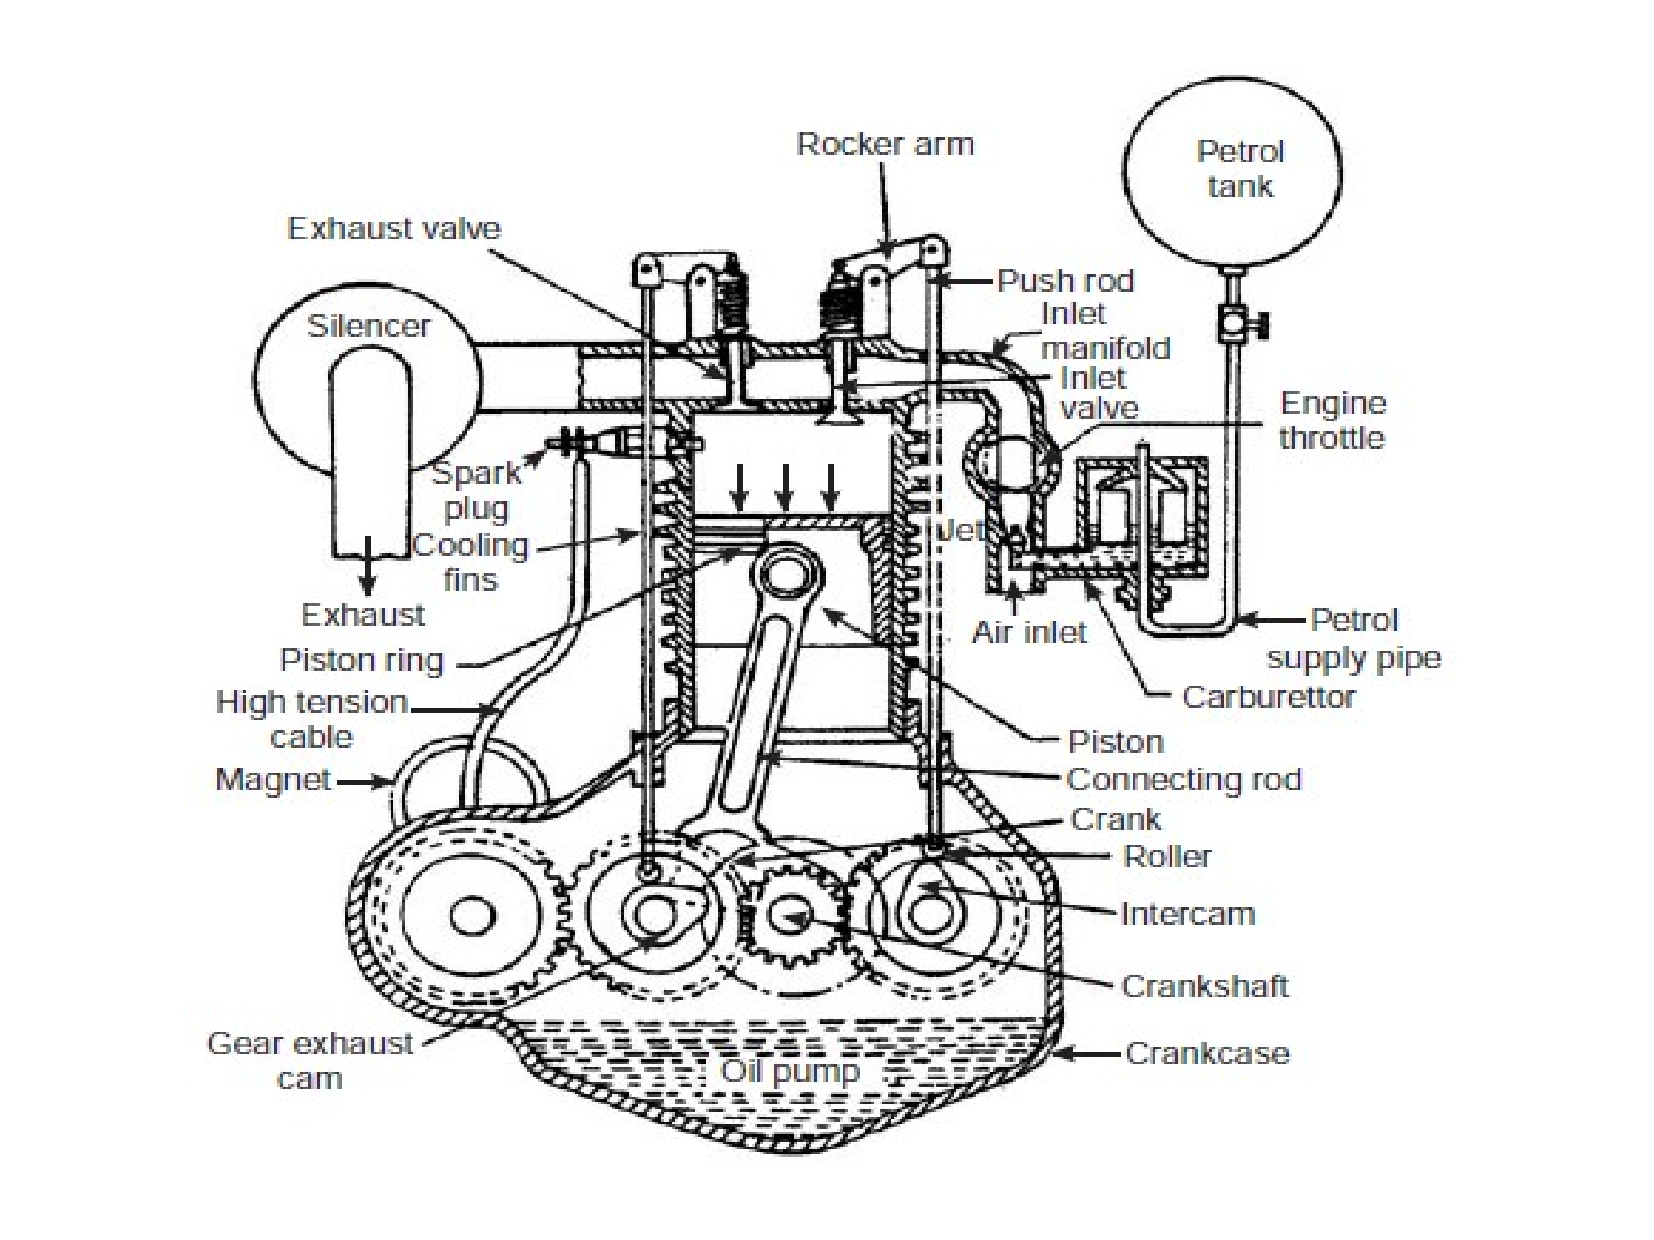
\includegraphics[width=7.5cm,clip]{./Pics/InternalCombustion_4Strokes}
      \caption{Air-cooled four-stroke petrol engine.}
     \end{center}
    \end{figure}  
   \end{column}  
  \end{columns}
\end{frame}


\subsection{Otto Cycle (Constant Volume)}
%%%
%%% Slide
%%%
\begin{frame}
 \frametitle{Four-Strokes Internal Combustion Engines}
  \begin{columns}
   \begin{column}[c]{0.4\linewidth}
    \begin{itemize}
     \item <1-> Fuel--air solution is compressed to a \textcolor{blue}{temperature just below the auto--ignition temperature of the fuel} and combustion is initialised by an electric spark;
     \item <2-> \textcolor{blue}{Suction stroke (SS):} also called \textcolor{blue}{intake stroke}. The mixture is injected through the intake valve (IV). The exhaust valve (EV) remains closed during this stage;
     \item <3-> \textcolor{blue}{Compression stroke} 
     \item <3-> \textcolor{blue}{Expansion stroke} 
     \item <3-> \textcolor{blue}{Exhaust stroke} 
    \end{itemize}
   \end{column}
   \begin{column}[c]{0.6\linewidth}
    \begin{figure}%
     \begin{center}
      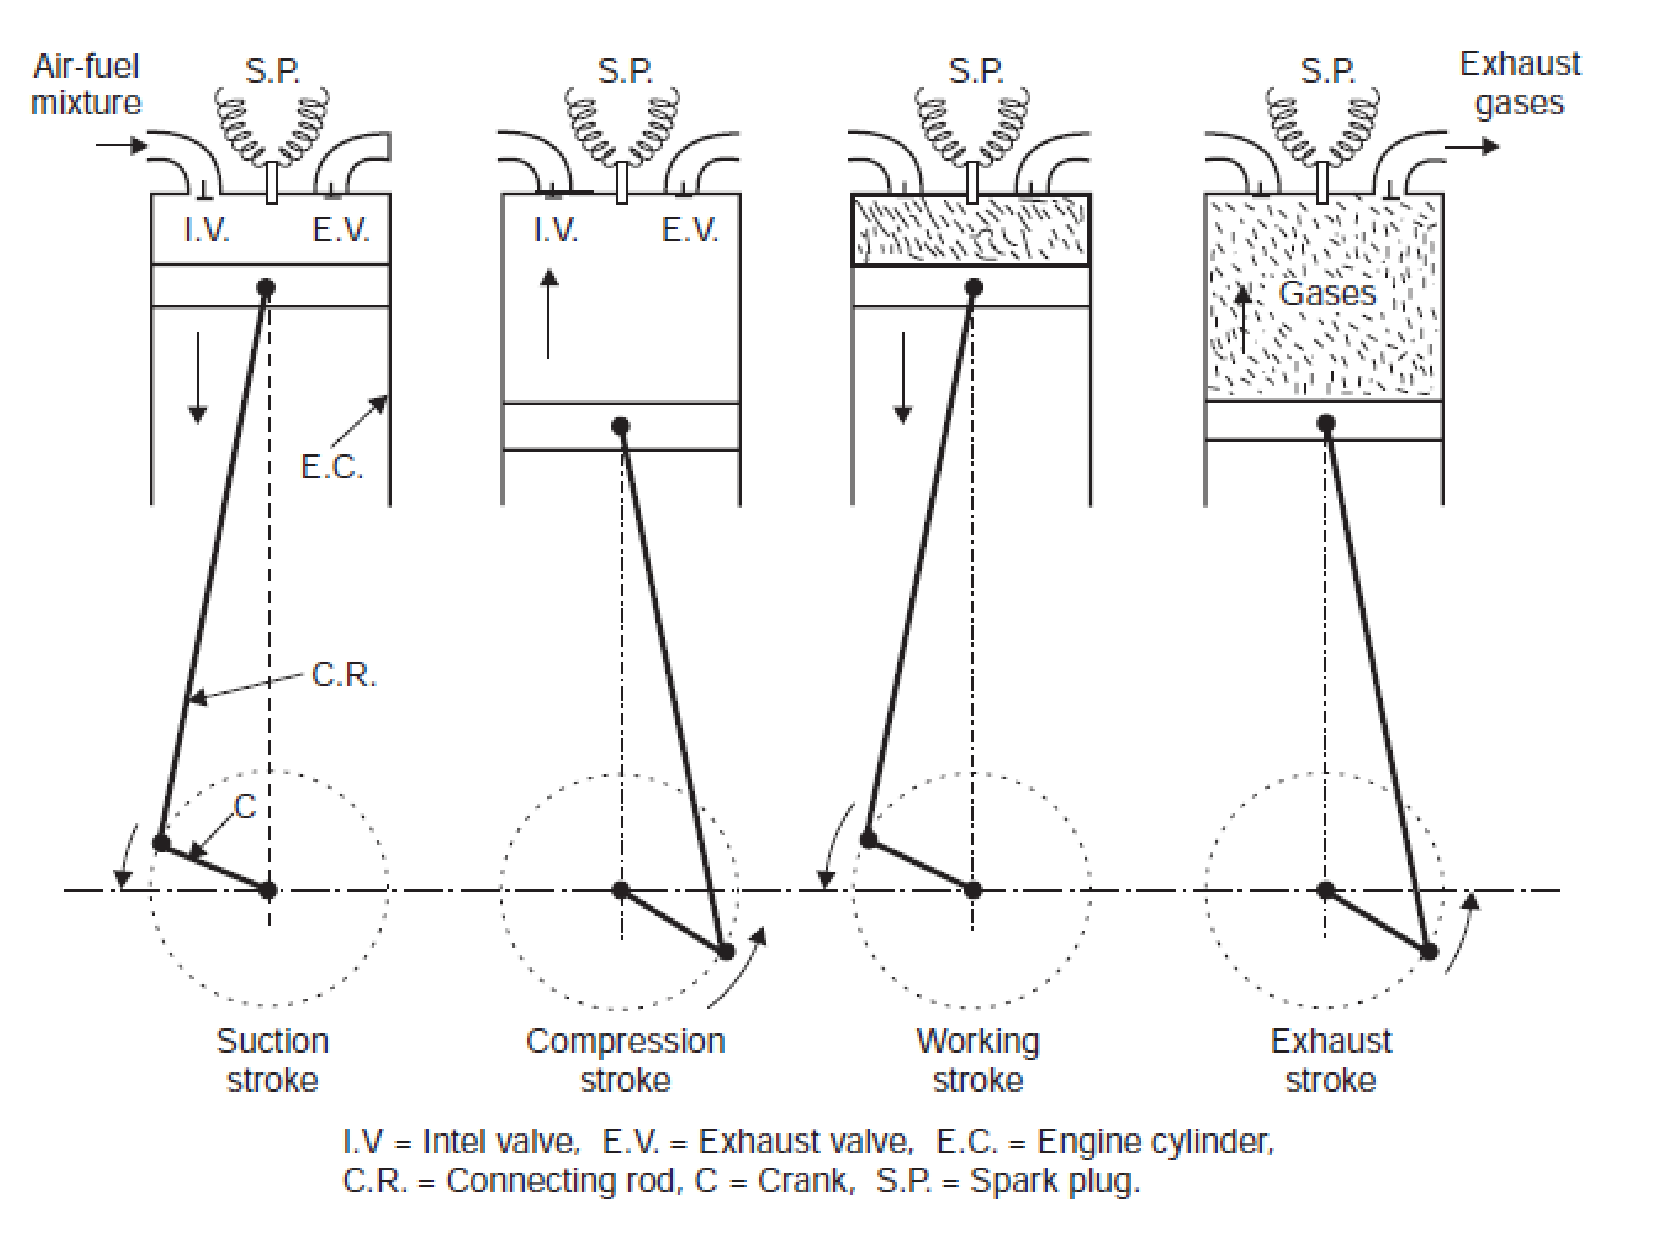
\includegraphics[width=7.5cm,clip]{./Pics/InternalCombustion_4Strokes_Otto}
      %\caption{Air-cooled four-stroke petrol engine.}
     \end{center}
    \end{figure}  
   \end{column}  
  \end{columns}
\end{frame}

%%%
%%% Slide
%%%
\begin{frame}
 \frametitle{Four-Strokes Internal Combustion Engines}
  \begin{columns}
   \begin{column}[c]{0.4\linewidth}
    \begin{itemize}
     \item <1-> \textcolor{blue}{Suction stroke (SS)} 
     \item <1-> \textcolor{blue}{Compression stroke (CS):} whereas IV and EV remain closed, pressure and temperature of the solution rise. Near the end of CS, the fuel is ignited by an electric spark, leading to the combustion of the fuel (consumption of carbon);
     \item <2-> \textcolor{blue}{Expansion stroke} 
     \item <2-> \textcolor{blue}{Exhaust stroke} 
    \end{itemize}
   \end{column}
   \begin{column}[c]{0.6\linewidth}
    \begin{figure}%
     \begin{center}
      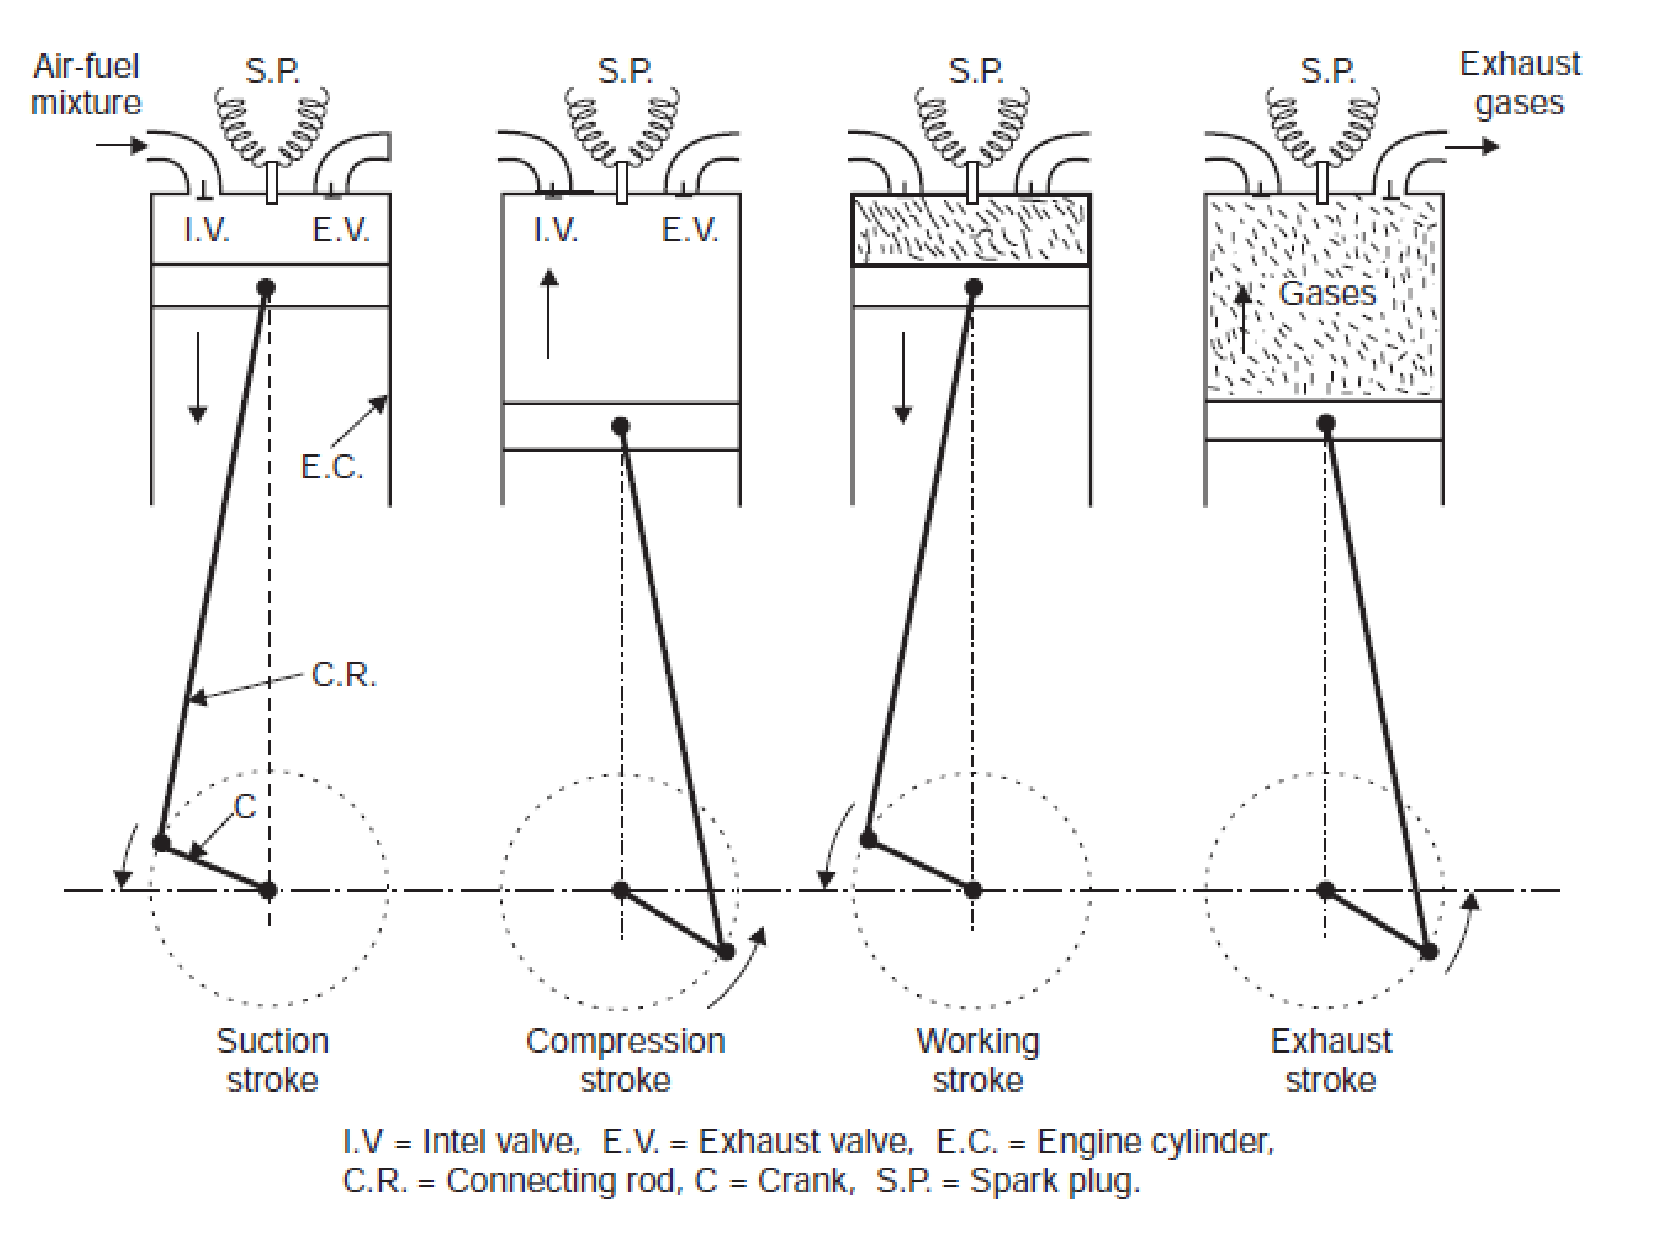
\includegraphics[width=7.5cm,clip]{./Pics/InternalCombustion_4Strokes_Otto}
      %\caption{Air-cooled four-stroke petrol engine.}
     \end{center}
    \end{figure}  
   \end{column}  
  \end{columns}
\end{frame}

%%%
%%% Slide
%%%
\begin{frame}
 \frametitle{Four-Strokes Internal Combustion Engines}
  \begin{columns}
   \begin{column}[c]{0.4\linewidth}
    \begin{itemize}
     \item <1-> \textcolor{blue}{Suction stroke (SS)} 
     \item <1-> \textcolor{blue}{Compression stroke (CS)} 
     \item <1-> \textcolor{blue}{Expansion stroke (WS):} also called \textcolor{blue}{power} or \textcolor{blue}{working} stroke. IV and EV remain closed and near the completion of the this stroke, the \textcolor{blue}{EV} is opened and the pressure in the cylinder push most of the gases out of the cylinder;
     \item <2-> \textcolor{blue}{Exhaust stroke} 
    \end{itemize}
   \end{column}
   \begin{column}[c]{0.6\linewidth}
    \begin{figure}%
     \begin{center}
      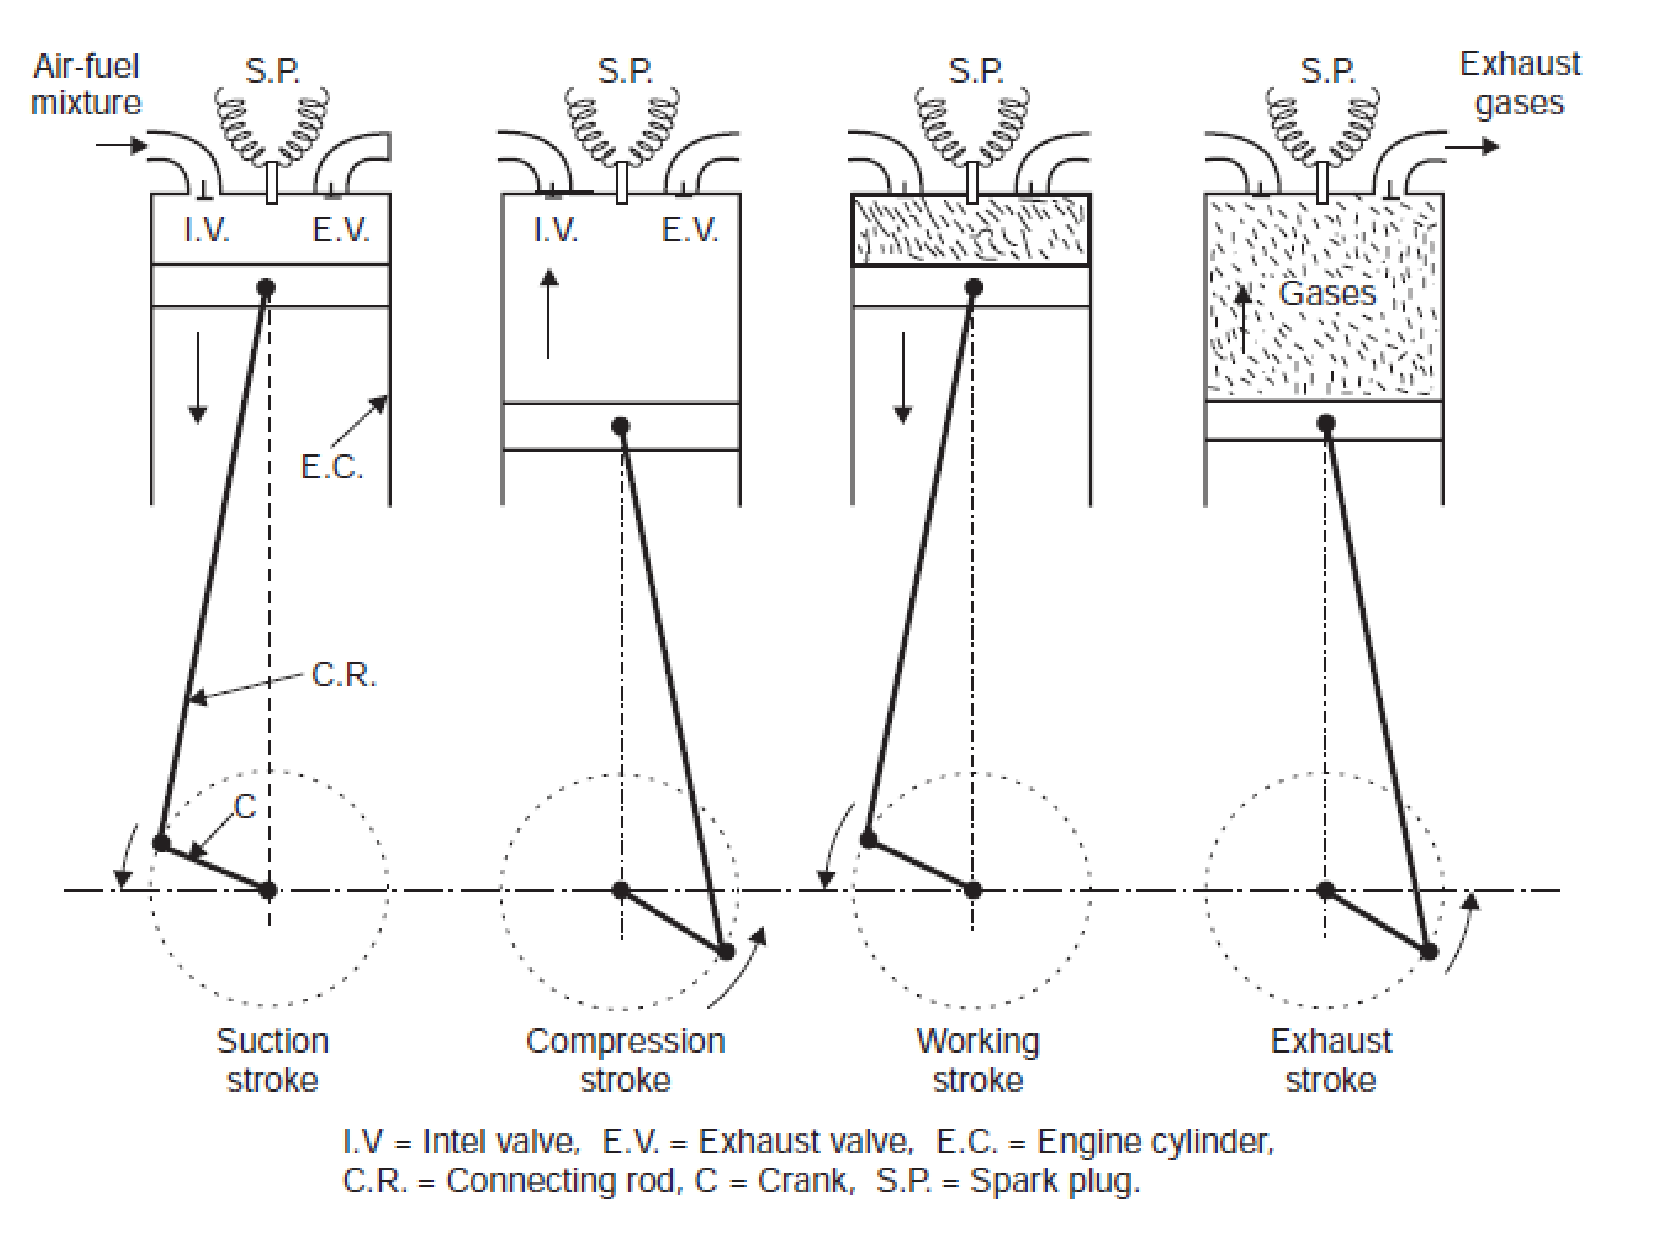
\includegraphics[width=7.5cm,clip]{./Pics/InternalCombustion_4Strokes_Otto}
      %\caption{Air-cooled four-stroke petrol engine.}
     \end{center}
    \end{figure}  
   \end{column}  
  \end{columns}
\end{frame}

%%%
%%% Slide
%%%
\begin{frame}
 \frametitle{Four-Strokes Internal Combustion Engines}
  \begin{columns}
   \begin{column}[c]{0.4\linewidth}
    \begin{itemize}
     \item <1-> \textcolor{blue}{Suction stroke (SS)} 
     \item <1-> \textcolor{blue}{Compression stroke (CS)} 
     \item <1-> \textcolor{blue}{Expansion stroke (WS)} 
     \item <1-> \textcolor{blue}{Exhaust stroke (ES):} all remaining gases are removed from the cylinder. While the IV remains closed the \textcolor{blue}{piston returns to the top dead centre (TDC)}.
    \end{itemize}
   \end{column}
   \begin{column}[c]{0.6\linewidth}
    \begin{figure}%
     \begin{center}
      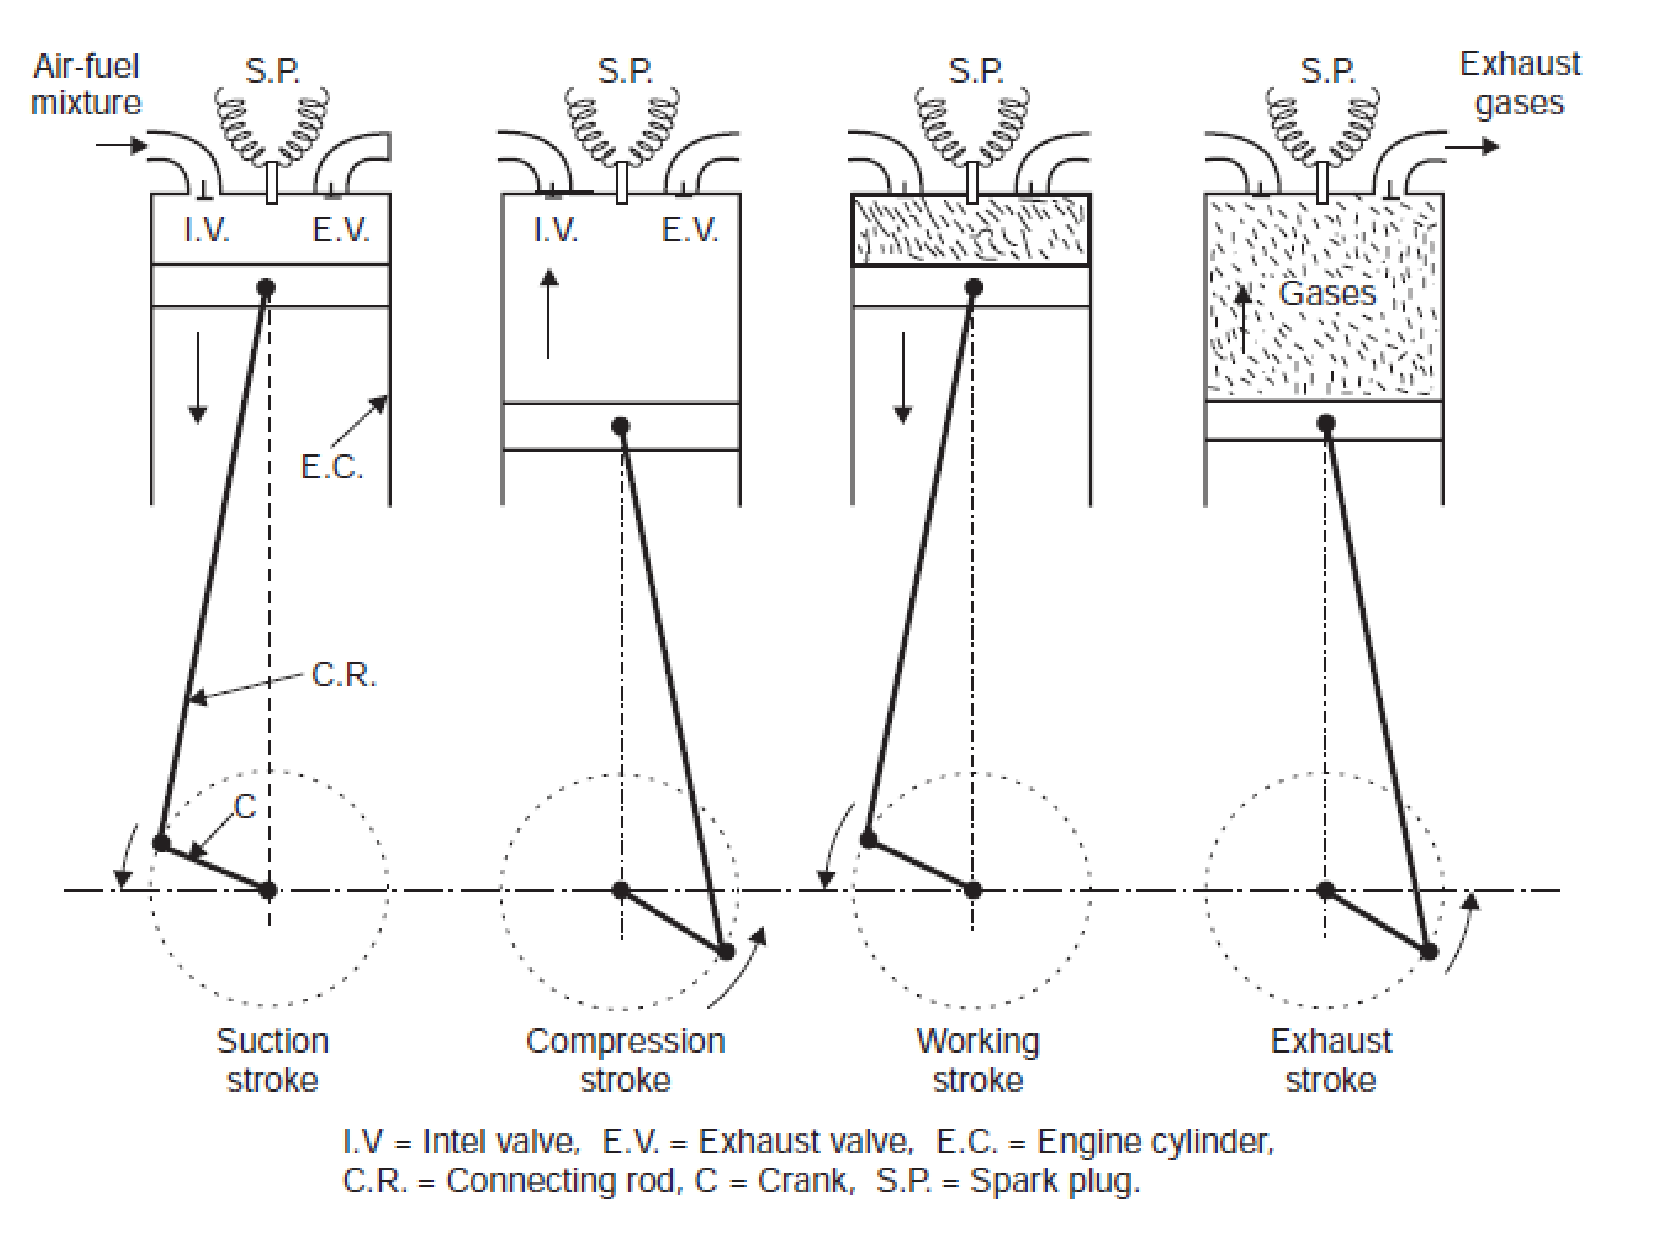
\includegraphics[width=7.5cm,clip]{./Pics/InternalCombustion_4Strokes_Otto}
      %\caption{Air-cooled four-stroke petrol engine.}
     \end{center}
    \end{figure}  
   \end{column}  
  \end{columns}
\textcolor{red}{Visualisation of the 4-strokes engine: \href{http://www.animatedengines.com/otto.html}{http://www.animatedengines.com/otto.html} }
\end{frame}

%%%
%%% Slide
%%%
\begin{frame}
 \frametitle{Two-Strokes Internal Combustion Engines}
  \begin{columns}
   \begin{column}[c]{0.4\linewidth}
    \begin{itemize}
     \item <1-> In this class of engines, \textcolor{blue}{both suction and exhaust strokes are eliminated};
     \item <2-> Valves are replaced by ports. 
     \item <3-> Exhaust gases are driven out of the cylinder by the fresh intake of mixing fuel + air \textcolor{blue}{at the end of the expansion stroke};
    \end{itemize}
   \end{column}
   \begin{column}[c]{0.6\linewidth}
    \begin{figure}%
     \begin{center}
      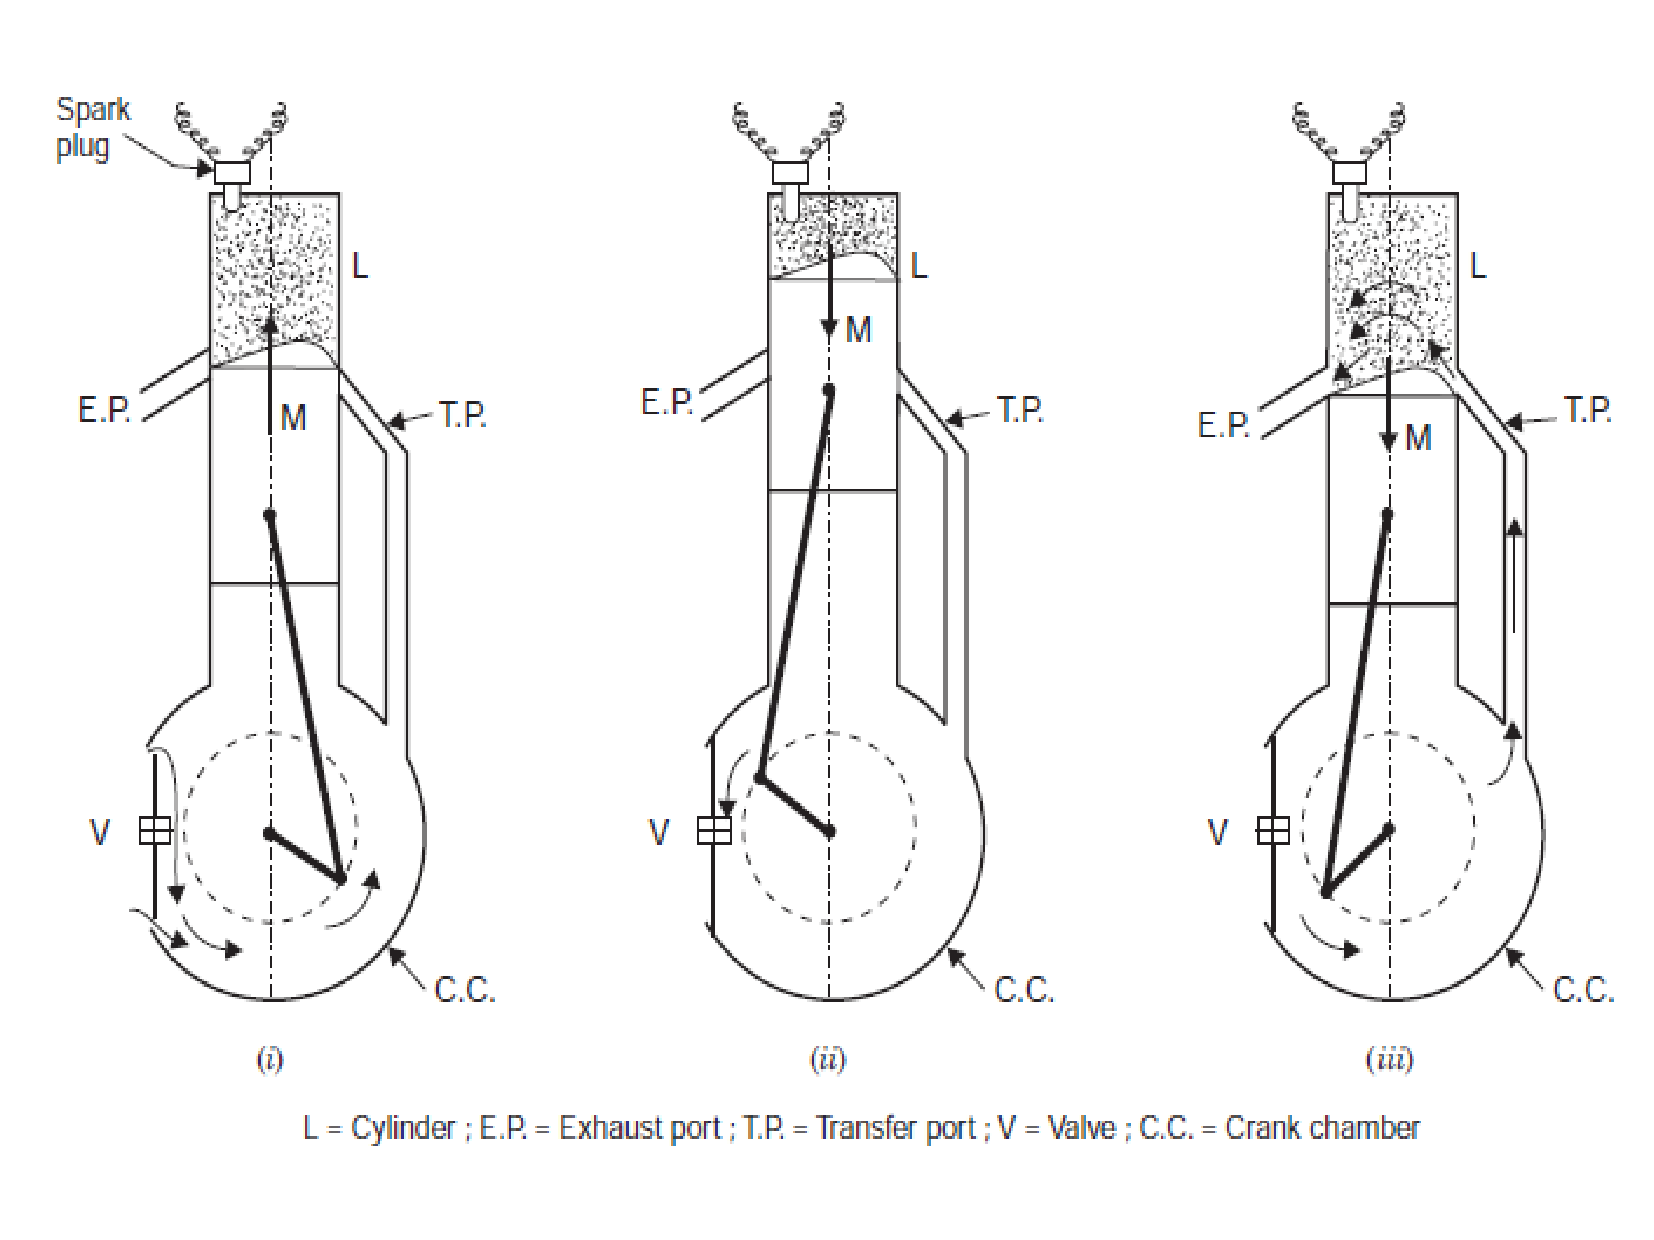
\includegraphics[width=7.5cm,clip]{./Pics/InternalCombustion_2Strokes_Otto}
      %\caption{Air-cooled four-stroke petrol engine.}
     \end{center}
    \end{figure}  
   \end{column}  
  \end{columns}
\end{frame}


%%%
%%% Slide
%%%
\begin{frame}
 \frametitle{Two-Strokes Internal Combustion Engines}
  \begin{columns}
   \begin{column}[c]{0.4\linewidth}
    \begin{enumerate}[(i)]
     \item <1-> Piston moves upwards compressing the fuel mixture (\textcolor{blue}{L}) previously supplied by \textcolor{blue}{V}. Ignition occurs in the end of the stroke (max compression);
     \item <2-> Piston moves downwards due to the gases expansion and near the end of the stroke, 
     \item <3-> Piston uncovers the \textcolor{blue}{exhausted port (EP)} and the gases are allowed to escape. The \textcolor{blue}{transfer port (TP)} is uncovered and the fresh fuel enters the cylinder driving away the remaining exhausted gases.
    \end{enumerate}
   \end{column}
   \begin{column}[c]{0.6\linewidth}
    \begin{figure}%
     \begin{center}
      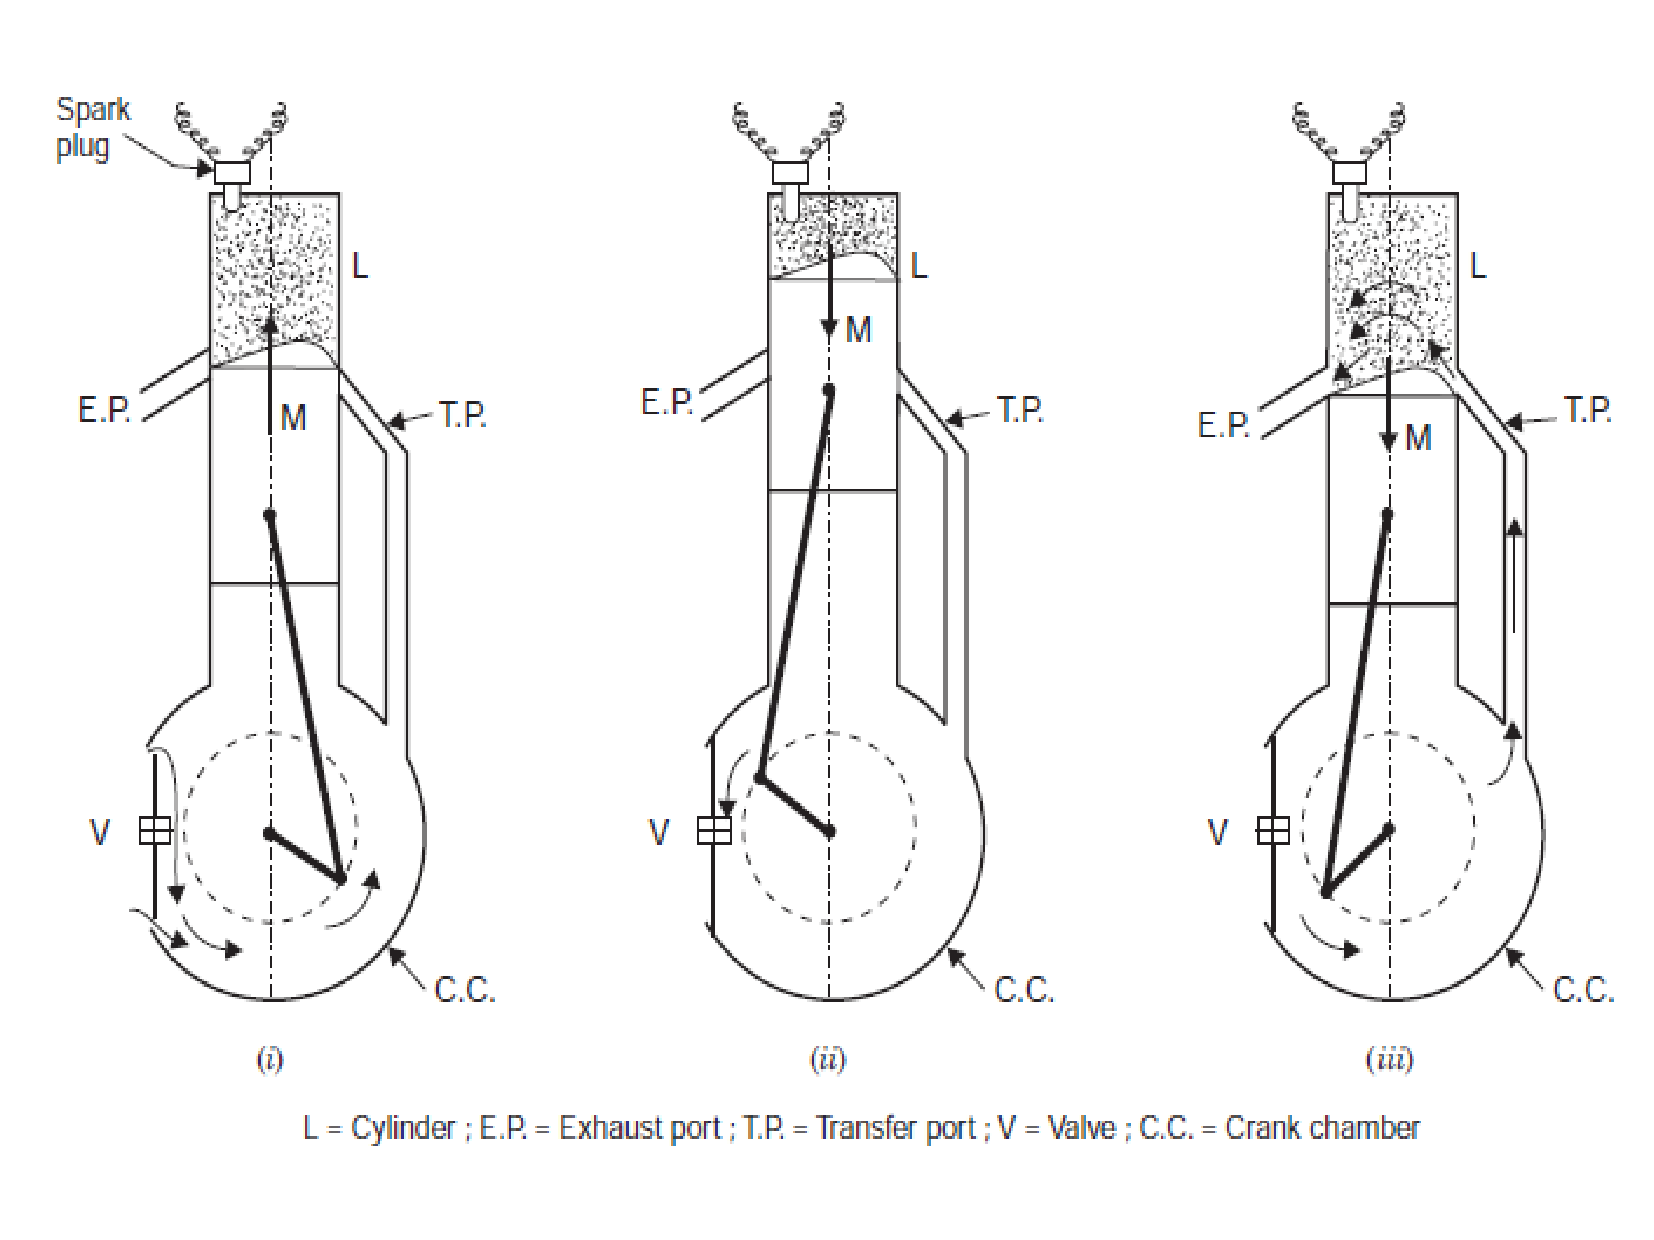
\includegraphics[width=7.5cm,clip]{./Pics/InternalCombustion_2Strokes_Otto}
      %\caption{Air-cooled four-stroke petrol engine.}
     \end{center}
    \end{figure}  
   \end{column}  
  \end{columns}
\end{frame}


%%%
%%% Slide
%%%
\begin{frame}
 \frametitle{Actual and Ideal Otto Cycles}
    Air-standard Otto cycle is an ideal cycle that assumes the heat addition occurs instantaneously while the piston is at TDC.
    \begin{figure}%
     \begin{center}
      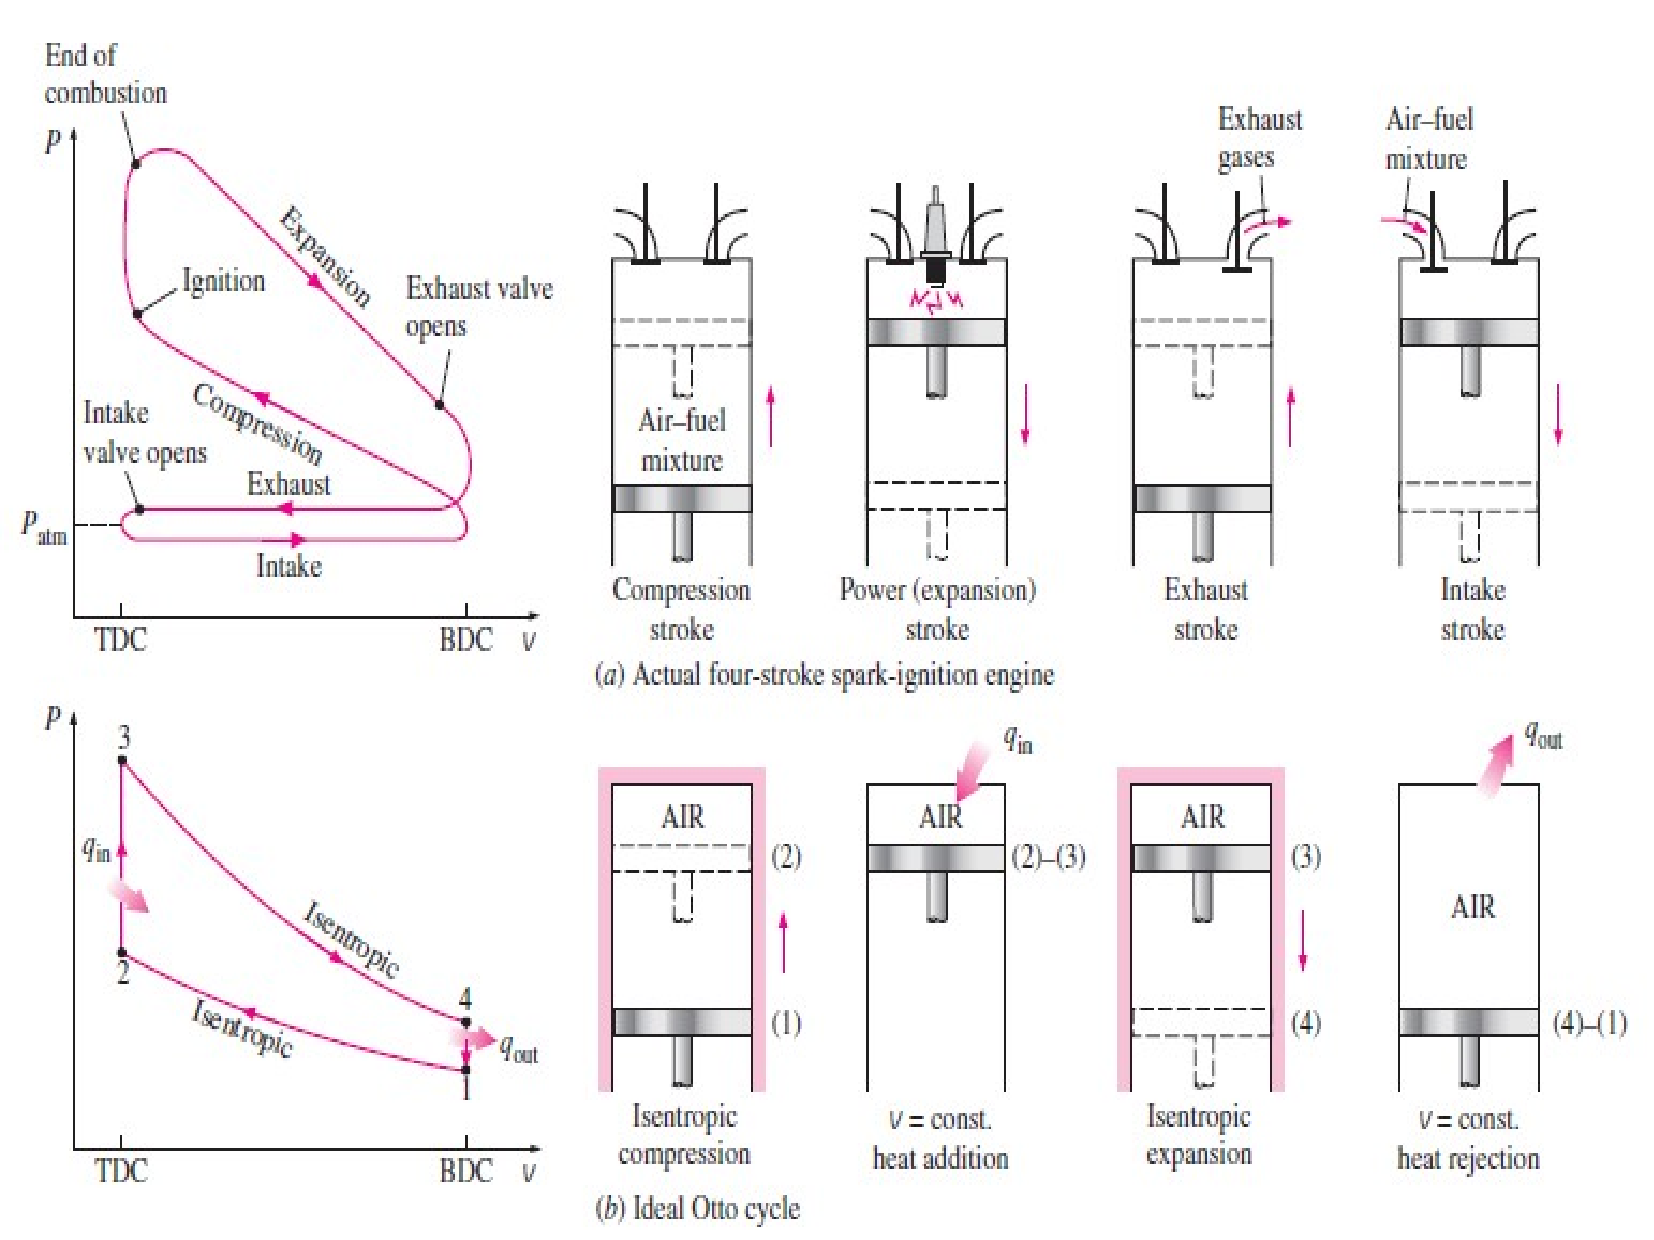
\includegraphics[width=9.cm,clip]{./Pics/InternalCombustion_IdealOttoCycle}
     %\caption{Actual and ideal cycles in SI engines and their associated Pv diagrams.}
     \end{center}
    \end{figure} 
\end{frame}

%%%
%%% Slide
%%%
\begin{frame}
 \frametitle{Ideal Otto Cycles}
  \begin{columns}
   \begin{column}[c]{0.4\linewidth}
    \begin{itemize}
     \item <1-> \textcolor{blue}{1-2:} Isentropic compression of air from $\left(P_{1},\;T_{1},\;V_{1}\right)$ to $\left(P_{2},\;T_{2},\;V_{2}\right)$;
     \item <2-> \textcolor{blue}{2-3:} Addition of heat, $Q_{in}$ at \textcolor{blue}{\it constant volume} from $\left(P_{2},\;T_{2},\;V_{2}\right)$ to $\left(P_{3},\;T_{3},\;V_{3}=V_{2}\right)$;
     \item <3-> \textcolor{blue}{3-4:} Isentropic expansion from $\left(P_{3},\;T_{3},\;V_{3}\right)$ to $\left(P_{4},\;T_{4},\;V_{4}=V_{1}\right)$;
     \item <4-> \textcolor{blue}{4-1:} Rejection of heat at \textcolor{blue}{\it constant volume} from $\left(P_{4},\;T_{4},\;V_{4}\right)$ to $\left(P_{1},\;T_{1},\;V_{1}\right)$. 
    \end{itemize}
   \end{column}
   \begin{column}[c]{0.6\linewidth}
    \begin{figure}%
     \begin{center}
      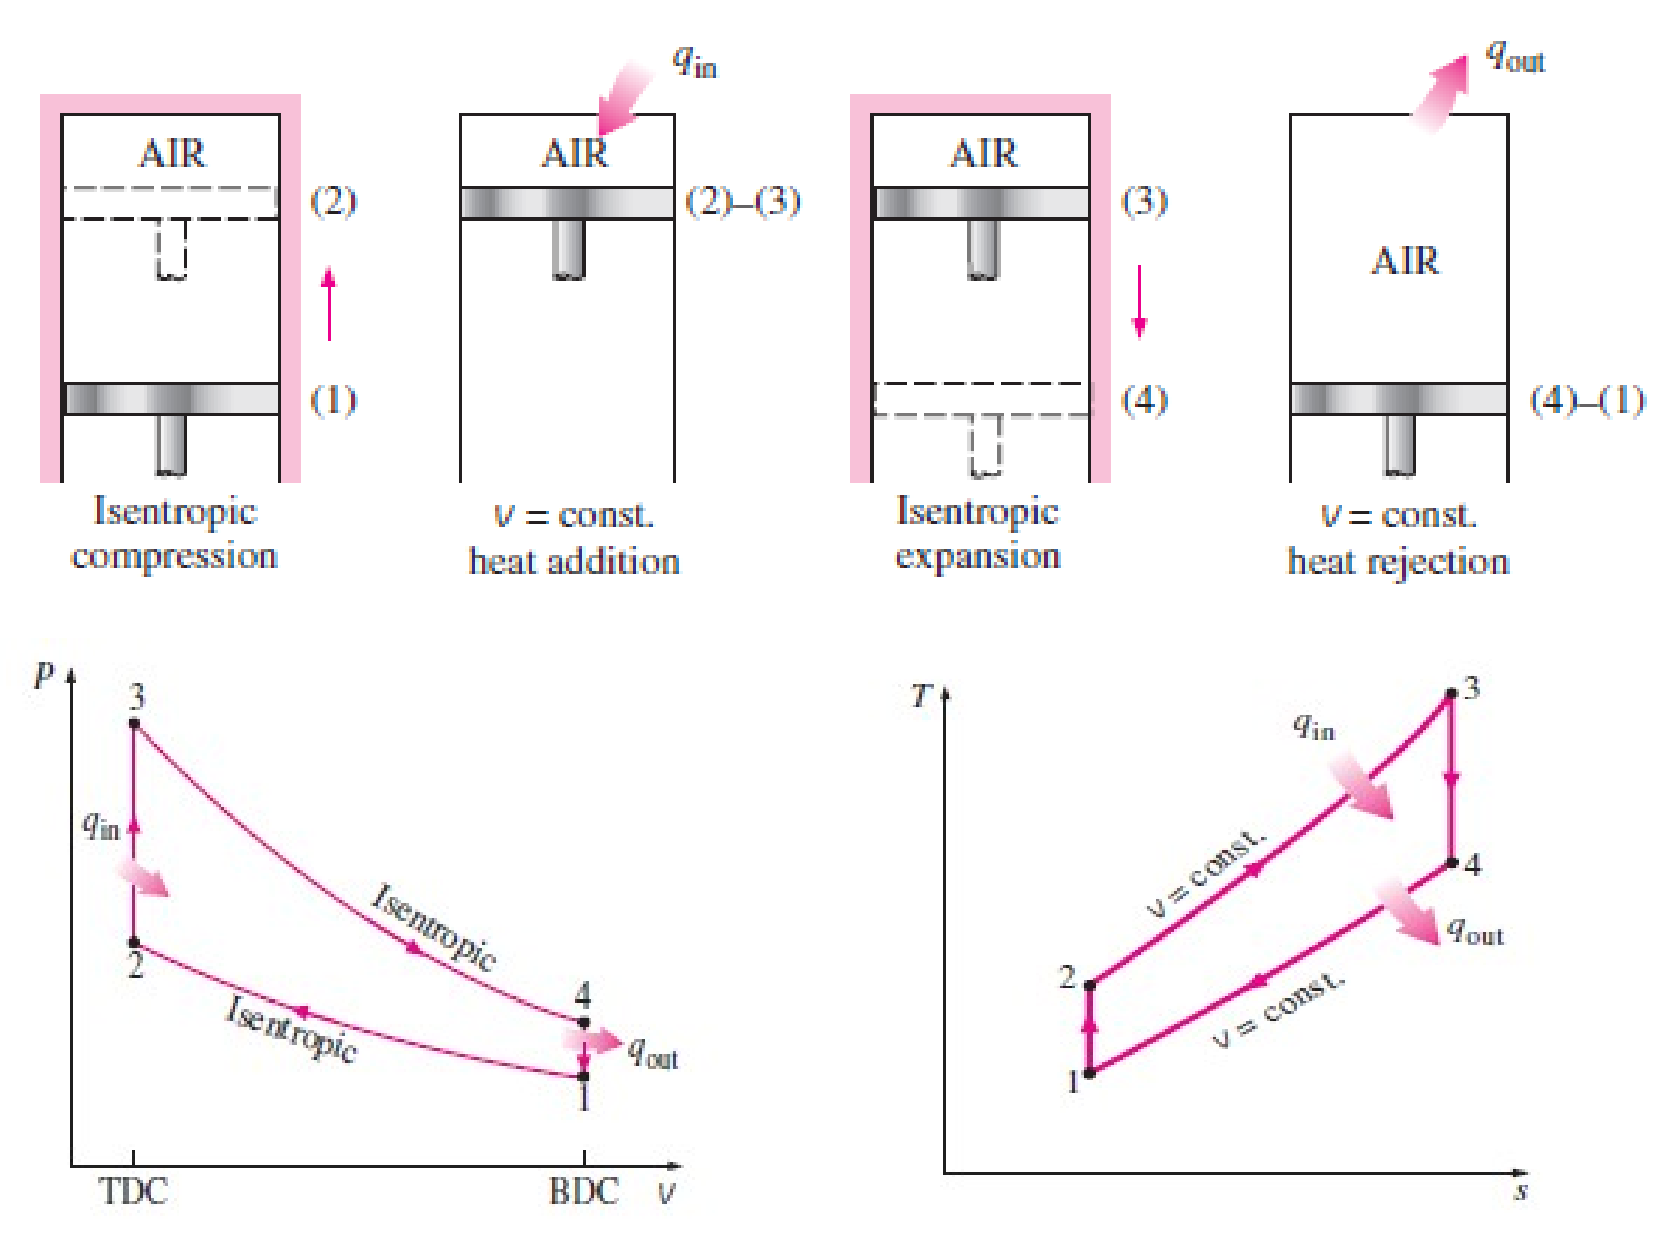
\includegraphics[width=7.5cm,clip]{./Pics/InternalCombustion_IdealOttoCycle2}
     \end{center}
    \end{figure}  
   \end{column}  
  \end{columns}
\end{frame}


%%%
%%% Slide
%%%
\begin{frame}
 \frametitle{Ideal Otto Cycles}
  \begin{columns}
   \begin{column}[c]{0.4\linewidth}
    \begin{itemize}
     \item <1-> Since ideal Otto cycle is composed of \textcolor{blue}{internally reversible processes}, areas on the {\it Ts} and {\it Pv} diagrams can be interpreted as \textcolor{blue}{heat and work};
     \item <2-> {\it Ts:} Area \textcolor{blue}{$2-3-b^{\prime}-a^{\prime}-2$} $\Rightarrow$ \textcolor{blue}{heat added per unit of mass} and;
     \item <3-> Area \textcolor{blue}{$1-4-b^{\prime}-a^{\prime}-1$} $\Rightarrow$ \textcolor{blue}{heat rejected per unit of mass};
     \item <4-> {\it Pv:} Area \textcolor{blue}{$3-4-b-a-3$} $\Rightarrow$  \textcolor{blue}{work done per unit of mass during the expansion} and;
    \end{itemize}
   \end{column}
   \begin{column}[c]{0.6\linewidth}
    \begin{itemize}
     \item <5-> Area \textcolor{blue}{$1-2-a-b-1$} $\Rightarrow$ \textcolor{blue}{work input per unit of mass during the compression};
     \item <6-> Enclosed area in the diagrams $\Rightarrow$ \textcolor{blue}{net work output (Pv)} and \textcolor{blue}{net heat added (Ts)}.
    \end{itemize}
    \begin{figure}%
     \begin{center}
      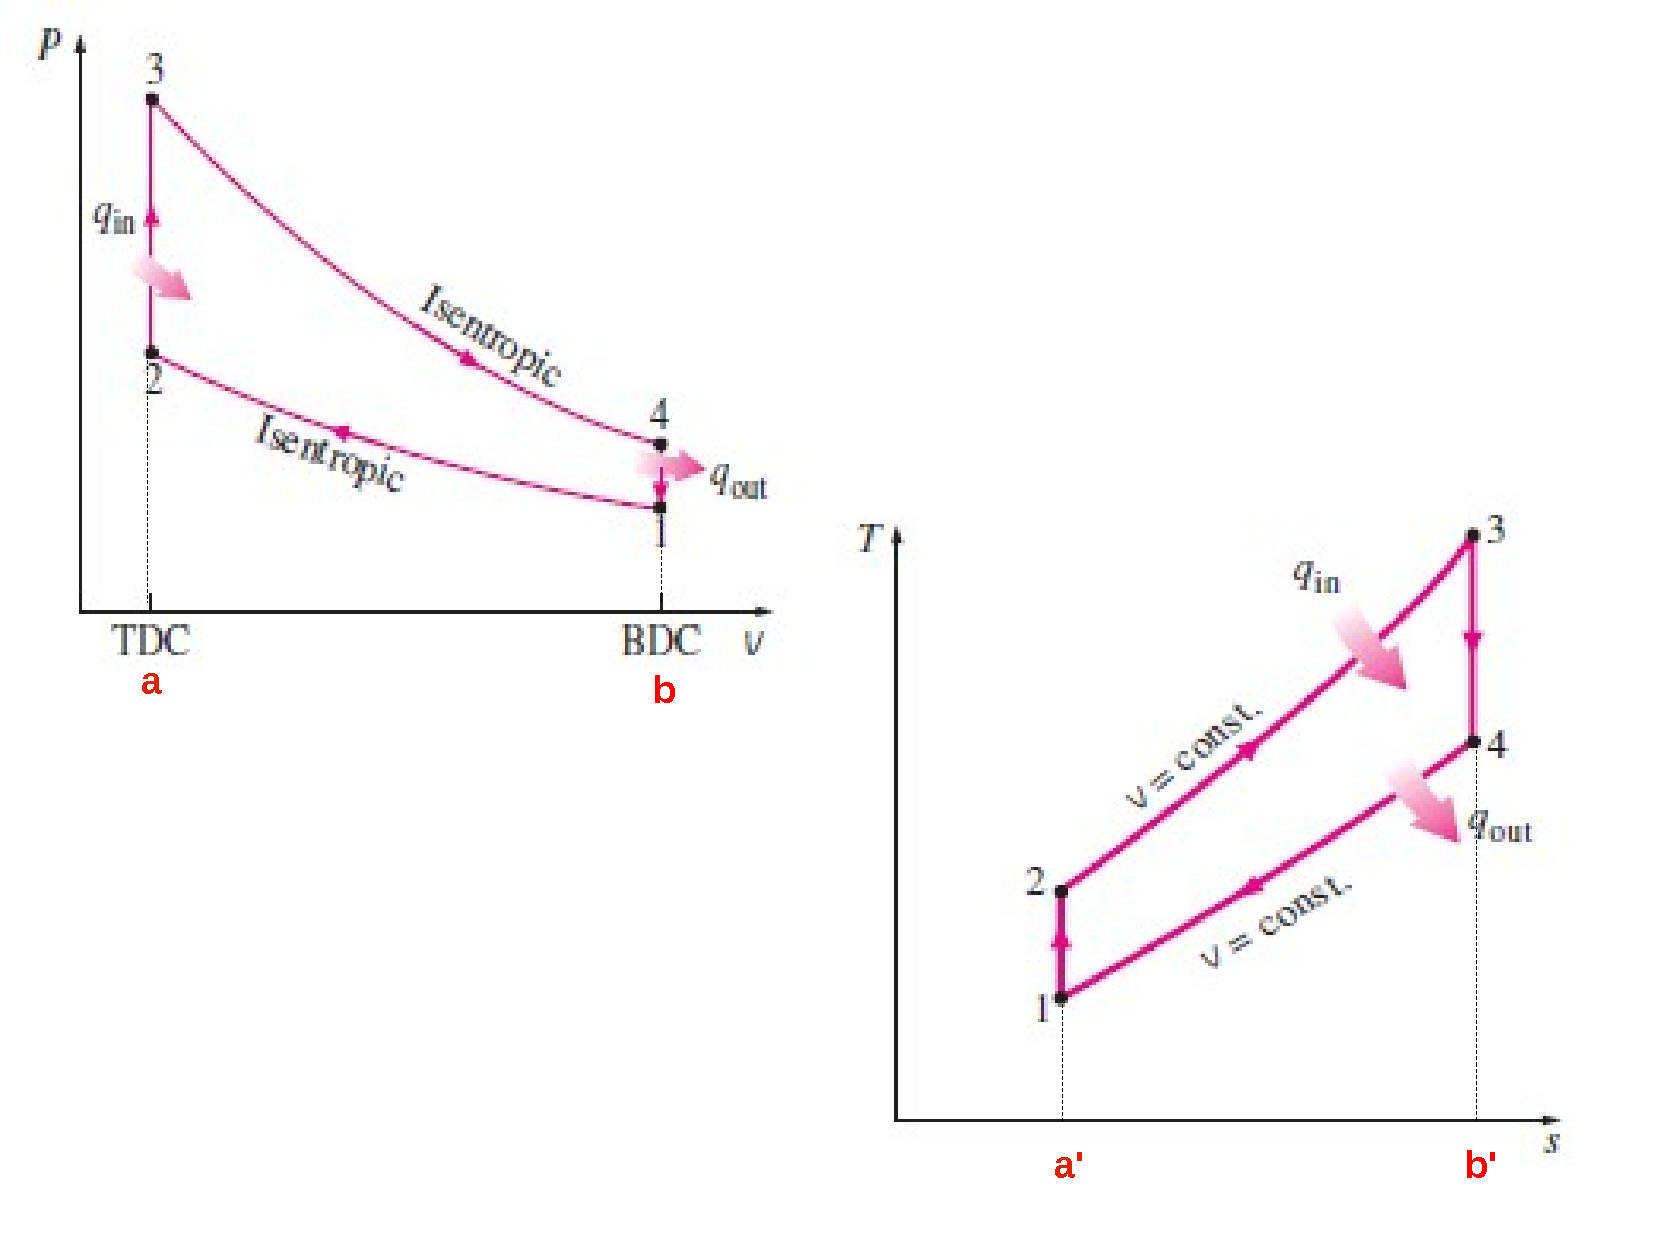
\includegraphics[width=7.cm,clip]{./Pics/InternalCombustion_IdealOttoCycle3}
     \end{center}
    \end{figure}  
   \end{column}  
  \end{columns}
\end{frame}

%%%
%%% Slide
%%%
\begin{frame}
 \frametitle{Ideal Otto Cycles}
   Thus the energy balance for 1 kg of air is
  \begin{itemize}
   \item <1-> Heat supplied at constant volume: $Q_{in}=C_{v}\left(T_{3}-T_{2}\right)$;
   \item <2-> Heat rejected at constant volume: $Q_{out}=C_{v}\left(T_{4}-T_{1}\right)$;
   \item <3-> Net Work = Heat supplied - Heat rejected: $W_{\text{net}}=C_{v}\left(T_{3}-T_{2}\right) - C_{v}\left(T_{4}-T_{1}\right)$
   \item <4-> Efficiency:
      \begin{eqnarray}
       \textcolor{blue}{\eta_{\text{Otto}}}&=& \displaystyle\frac{W_{\text{net}}}{Q_{in}}=\displaystyle\frac{C_{v}\left(T_{3}-T_{2}\right) - C_{v}\left(T_{4}-T_{1}\right)}{C_{v}\left(T_{3}-T_{2}\right)} \nonumber \\
                       &=& \textcolor{blue}{1 - \displaystyle\frac{T_{4}-T_{1}}{T_{3}-T_{2}}} \nonumber% \\
                       %&=& 1 - \displaystyle\frac{T_{1}\left(\displaystyle\frac{T_{4}}{T_{1}}-1\right)}{T_{2}\left(\displaystyle\frac{T_{3}}{T_{2}}-1\right)}\nonumber 
      \end{eqnarray}
  \end{itemize}
\end{frame}

%%%
%%% Slide
%%%
\begin{frame}
 \frametitle{Ideal Otto Cycles}
  \begin{itemize}
   \item <1-> Compression ratio: $r_{c}=\displaystyle\frac{V_{1}}{V_{2}} = r$ and;
   \item <2-> Expansion ratio: $r_{e}=\displaystyle\frac{V_{4}}{V_{3}} = r$;
   \item <3-> As processes \textcolor{blue}{1--2} and \textcolor{blue}{3--4} are \textcolor{blue}{isentropic}, i.e., 
              \begin{displaymath}
               \displaystyle\frac{T_{2}}{T_{1}} = \left( \displaystyle\frac{V_{1}}{V_{2}} \right)^{\gamma - 1} = r^{\gamma - 1} \;\;\text{and }\;\; \displaystyle\frac{T_{3}}{T_{4}} = \left( \displaystyle\frac{V_{4}}{V_{3}} \right)^{\gamma - 1} = r^{\gamma - 1}
              \end{displaymath}
   \item <4-> and $V_{2}=V_{3}$ and $V_{4}=V_{1}$. Replacing $T_{2}$ and $T_{3}$ from above in $\eta_{\text{Otto}}$ expression:
              \begin{displaymath}
                \textcolor{blue}{\eta_{\text{Otto}}} = 1 - \displaystyle\frac{T_{4}-T_{1}}{T_{4} r^{\gamma-1}-T_{1} r^{\gamma-1}} = \textcolor{blue}{1 - \displaystyle\frac{1}{r^{\gamma-1}}}
              \end{displaymath}
     This expression is called the \textcolor{blue}{air-standard efficiency of the Otto cycle}.
   %\item <4->  
  \end{itemize}
\end{frame}

%%%
%%% Slide
%%%
\begin{frame}
 \frametitle{Ideal Otto Cycles}
  \begin{columns}
   \begin{column}[c]{0.3\linewidth}
    \begin{itemize}
     \item <1-> $\gamma=1.4\;\;\Longrightarrow$ ambient air;
     \item <2-> For gasoline engines: \\
 6.5$\leq r \leq$ 10
    \end{itemize}
   \end{column}
   \begin{column}[c]{0.7\linewidth}
    \begin{figure}%
     \begin{center}
      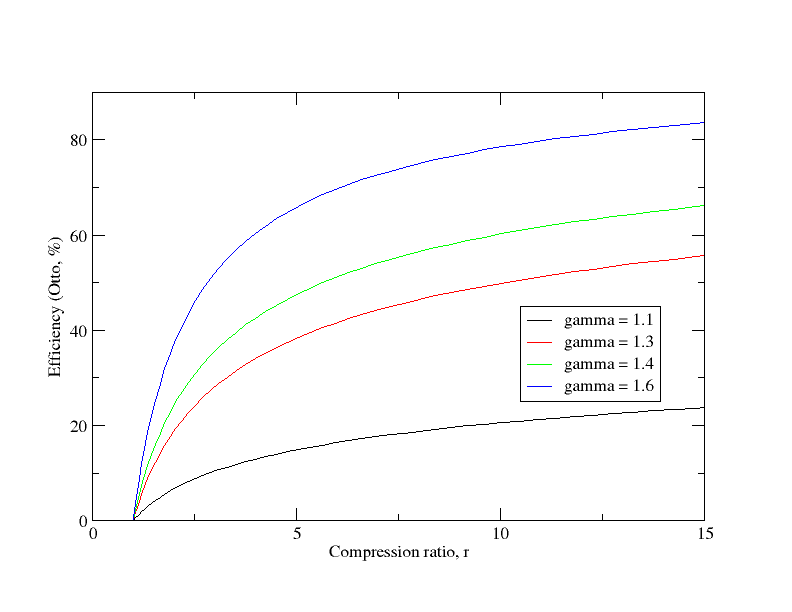
\includegraphics[width=9.cm,clip]{./Pics/Otto_Effic_CompRatio.png}
     \end{center}
    \end{figure}   
   \end{column}  
  \end{columns}
\end{frame}

%%%
%%% Slide
%%%
\begin{frame}
 \frametitle{Ideal Otto Cycles}
 \begin{itemize}
  \item <1-> Remember that the mean effective pressure is defined as
   \begin{displaymath}
    MEP = \displaystyle\frac{W_{\text{net}}}{V_{\text{max}}-V_{\text{min}}}
   \end{displaymath}
  \item<2-> where the net work can be expressed as a function of $P\;\left(\text{in bar}\right)$ and $V$
   \begin{displaymath}
     W_{\text{net}} = \displaystyle\frac{P_{1}V_{1}}{\gamma - 1}\left[\left(r^{\gamma-1}-1\right)\left(r_{p}-1\right)\right]
   \end{displaymath}
  \item<3-> with the \textcolor{blue}{presssure ratio}, $r_{p}=\displaystyle\frac{P_{3}}{P_{2}}=\displaystyle\frac{P_{4}}{P_{1}}$,
   \begin{displaymath}
    \textcolor{blue}{MEP = \displaystyle\frac{P_{1}r\left[\left(r^{\gamma-1} - 1\right)\left(r_{p}-1\right)\right]} {\left(\gamma-1\right)\left(r-1\right)}}
   \end{displaymath}
   
 \end{itemize}
\end{frame}


%%%
%%% Slide
%%%
\begin{frame}
 \frametitle{Ideal Otto Cycles -- Example}
\textcolor{blue}{An engine of 250 mm bore and 375 mm stroke works on ideal Otto cycle. The clearance volume is 0.00263 m$^{3}$. The initial pressure and temperature are 1 bar and 50$^{\text{o}}$C. If the maximum pressure is limited to 25 bar, determine: (a) air standard efficiency of the cycle and (b) MEP.}

\medskip

\begin{tabular}{c c l}
Given:    &                  &            \\
          & Bore             & $D = 2.5\times 10^{-1}\;m$  \\
          & Stroke length    & $L = 3.75\times 10^{-1}\;m$ \\
          & Clearence Volume & $V_{c} = 2.63\times 10^{-3}\;m^{3}$ \\
          & Initial Pressure & $P_{1}= 1\;bar$   \\
          & Initial Temperature & $T_{1}=323.15\;K$ \\
          & Maximum Pressure & $P_{3}=25\;bar$\\
Calculate:&                  & \\
          & $\eta_{\text{Otto}}$ & \\
          & MEP              & \\
\end{tabular}

\end{frame}


%%%
%%% Slide
%%%
\begin{frame}
 \frametitle{Ideal Otto Cycles --  Example}
  \begin{columns}
   \begin{column}[c]{0.6\linewidth}
    \begin{itemize}
     \item <1-> Swept volume: $V_{s}=\displaystyle\frac{\pi}{4}D^{2}L=1.84\times 10^{-2}\;m^{3}$;
     \item <2-> Compression ratio: $r=\displaystyle\frac{V_{s}+V_{c}}{V_{c}}=8$;
     \item <3-> The air-standard efficiency,
      \begin{displaymath}
       \eta_{\text{Otto}} = 1 - \displaystyle\frac{1}{r^{\gamma-1}}=0.565
      \end{displaymath}
     \item <4-> For the adiabatc (or isentropic) process 1-2, $P_{1}V_{1}^{\gamma}=P_{2}V_{2}^{\gamma}$ $\Rightarrow$ $P_{2}=18.38\;bar$
     \item <5-> and the pressure ratio, $r_{p}=\displaystyle\frac{P_{3}}{P_{2}}=1.36$
     \item <6-> Finally, we can calculate the mean effective pressure,
       \begin{displaymath}
        MEP = \displaystyle\frac{P_{1}r\left[\left(r^{\gamma-1} - 1\right)\left(r_{p}-1\right)\right]} {\left(\gamma-1\right)\left(r-1\right)} = 1.334\;bar
       \end{displaymath}
    \end{itemize}
   \end{column}
   \begin{column}[c]{0.4\linewidth}
    \begin{figure}%
     \begin{center}
      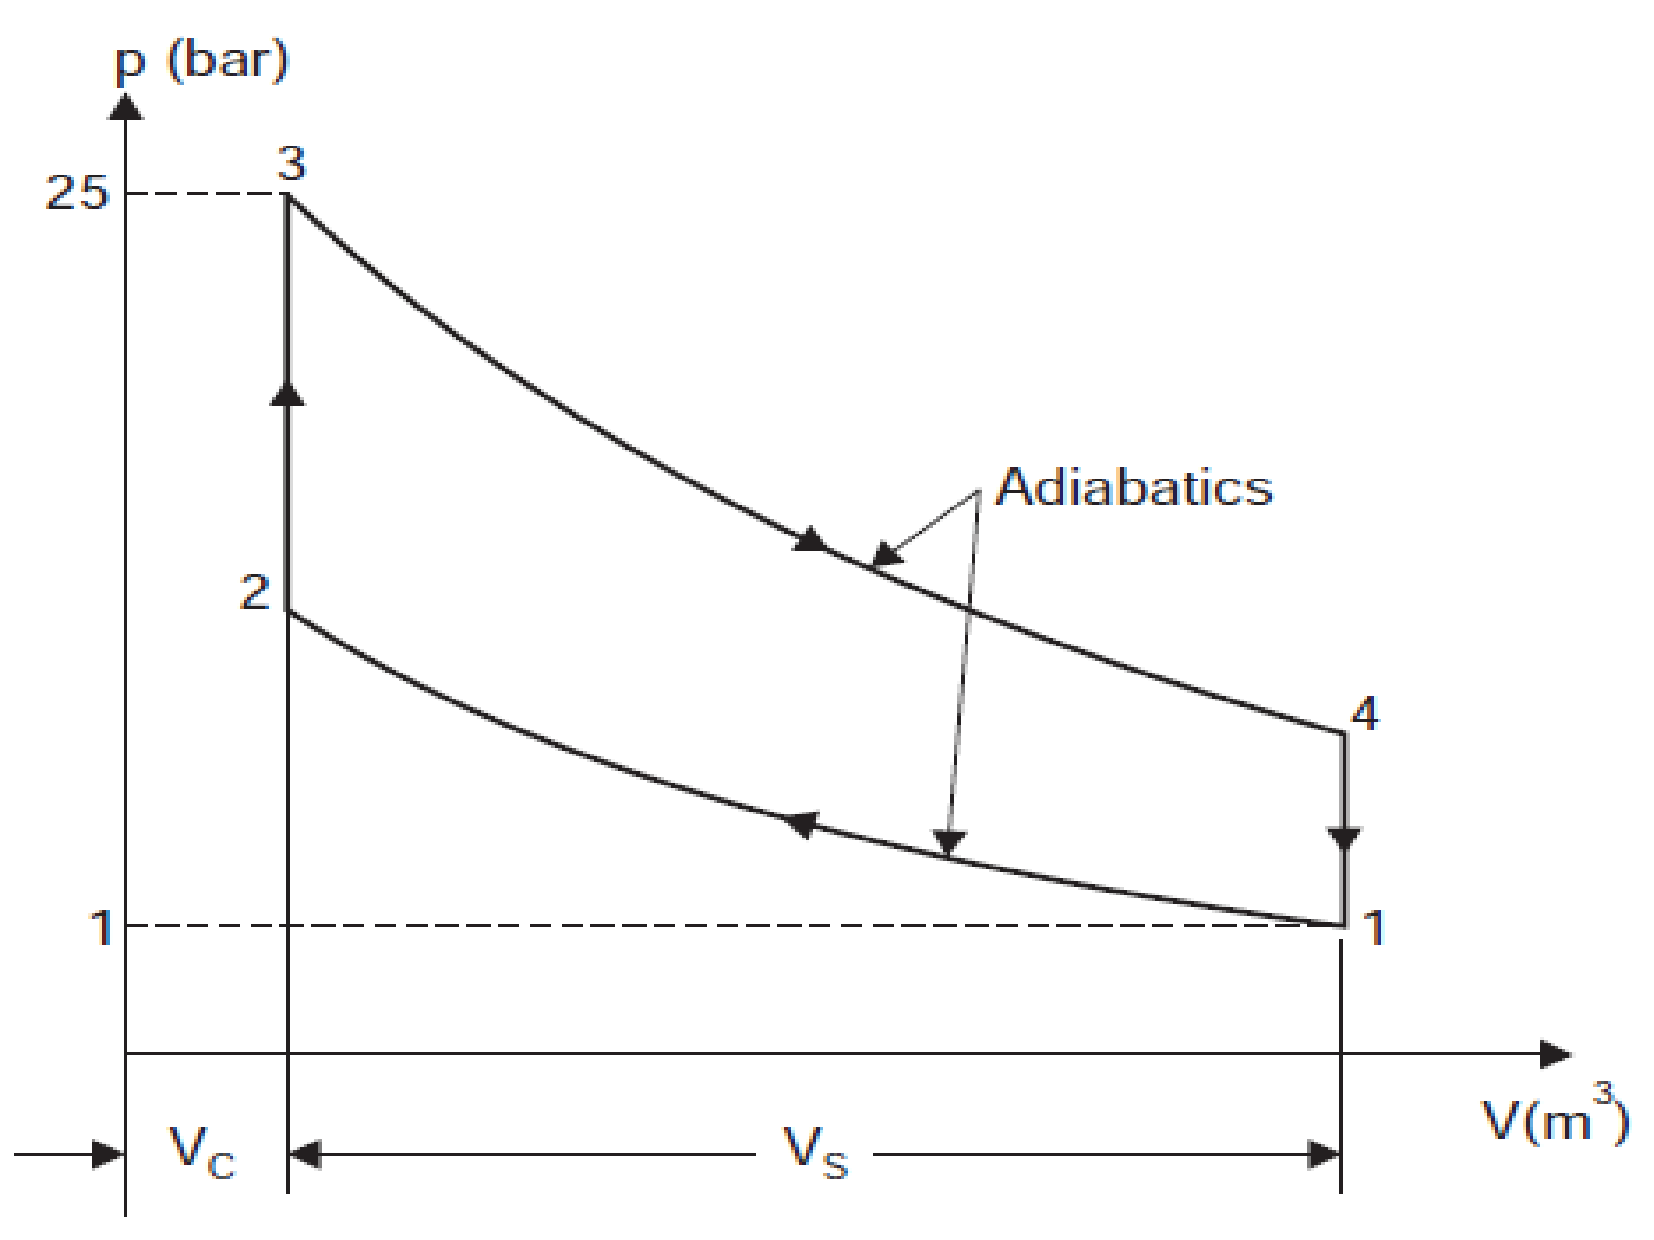
\includegraphics[width=5.cm,clip]{./Pics/InternalCombustion_IdealOttoCycle_Example1}
     \end{center}
    \end{figure}   
   \end{column}  
  \end{columns}
\end{frame}



\subsection{Diesel Cycle (Constant Pressure)}
%%%
%%% Slide
%%%
\begin{frame}
 \frametitle{Ideal Diesel Cycles}
  \begin{columns}
   \begin{column}[c]{0.5\linewidth}
    \begin{itemize}
     \item <1-> The Diesel cycle is the ideal cycle for \textcolor{blue}{compression-ignition} reciprocating engines;
     \item <2-> \textcolor{blue}{Only air is compressed} in the {\it compression stroke} -- eliminating the possibility of autoignition;
     \item <3-> Combustion starts on contact as the fuel is injected into the hot air \textcolor{blue}{$\left(T>T^{\text{fuel}}_{\text{auto-ignition}}\right)$}, 
     \item <4-> The spark plug and carburetor are replaced by fuel injector in diesel engines;
     \item <5-> Diesel engines can be designed to operate at \textcolor{blue}{much higher compression ratios} -- typically 12$\leq$r$\leq$24.
    \end{itemize}
   \end{column}
   \begin{column}[c]{0.5\linewidth}
    \begin{figure}%
     \begin{center}
      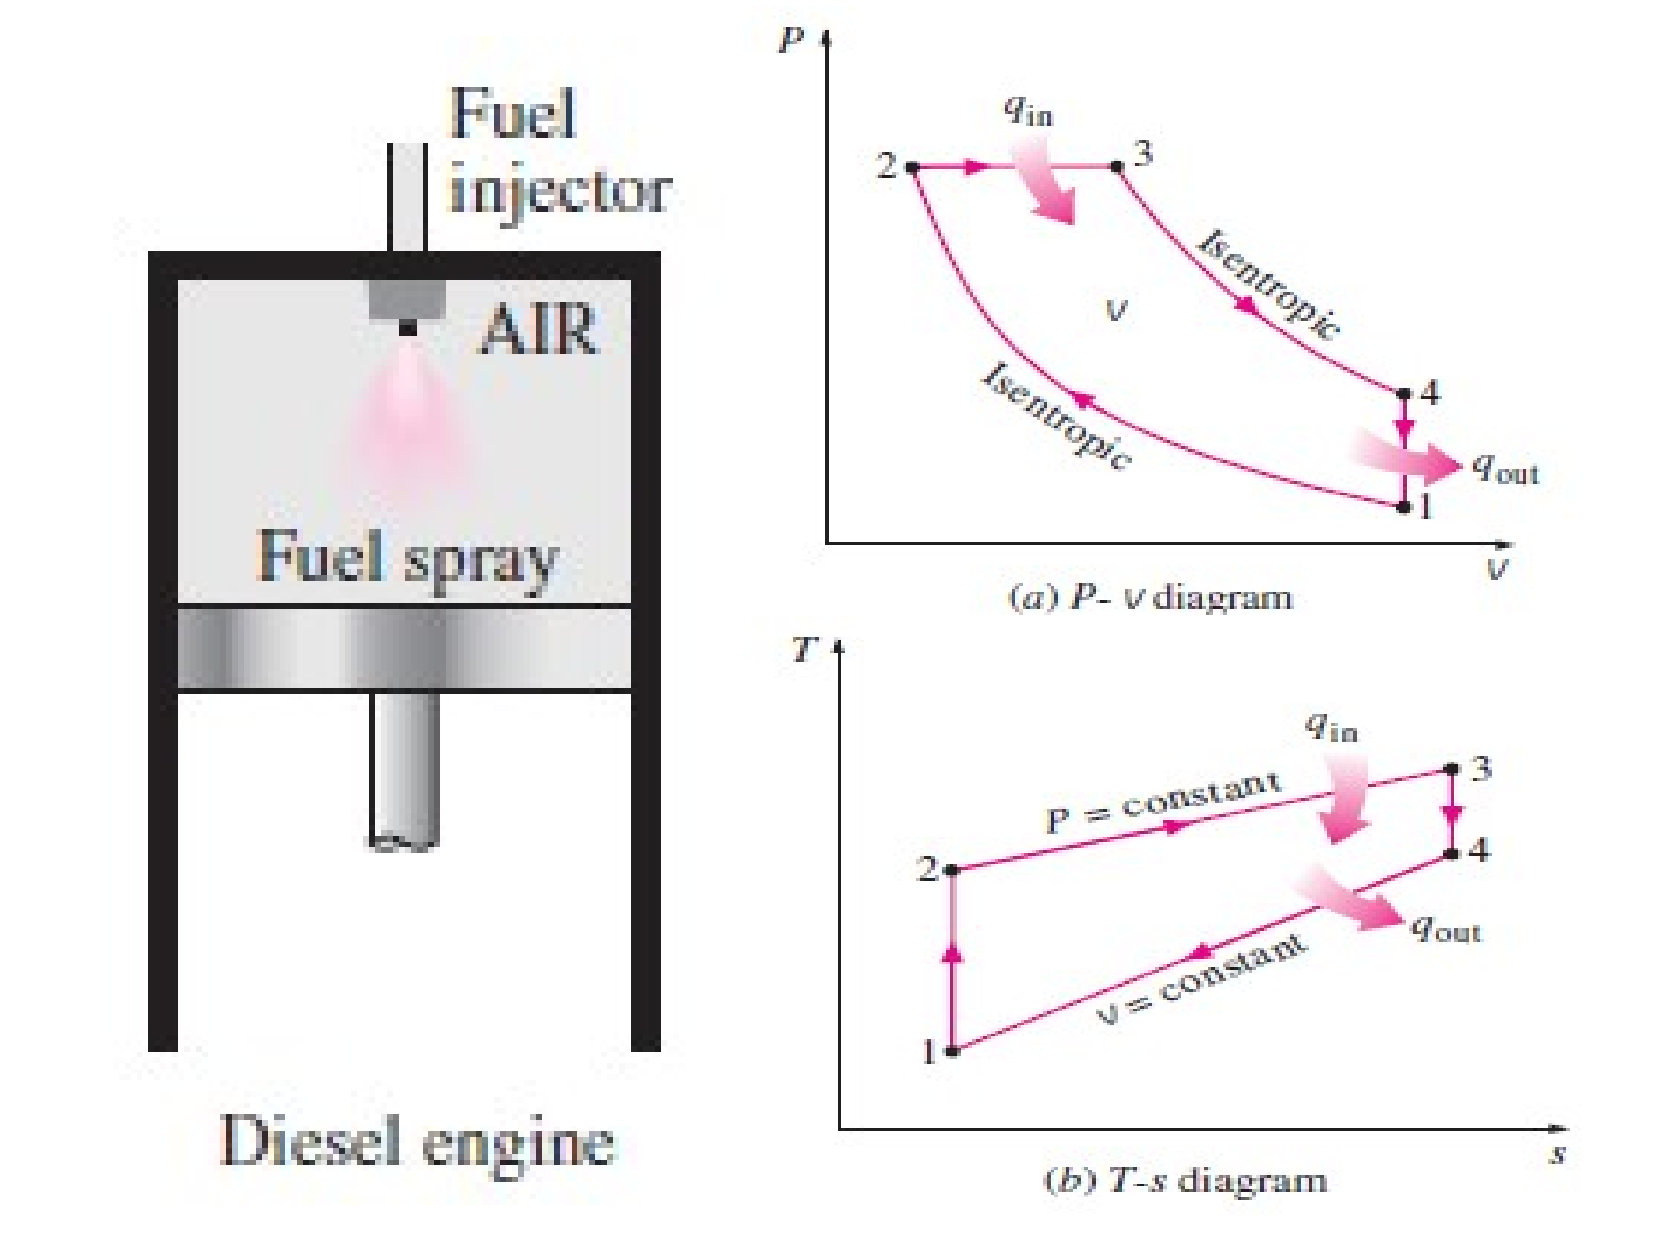
\includegraphics[width=6.cm,clip]{./Pics/InternalCombustion_IdealDieselCycle}
     \end{center}
    \end{figure}   
   \end{column}  
  \end{columns}
\end{frame}

%%%
%%% Slide
%%%
\begin{frame}
 \frametitle{Ideal Diesel Cycles}
  \begin{columns}
   \begin{column}[c]{0.5\linewidth}
    \begin{itemize}
     \item <1-> Fuel injection in diesel engines starts when the piston approaches TDC and;
     \item <2-> Continues during the first part of the expansion stroke;
     \item <3-> Combustion process occurs over a longer interval and, therefore the cycle can be approximated as a constant-pressure heat-addition process;
     \item <4-> \textcolor{red}{this is the only difference between Otto and Diesel cycles}.
    \end{itemize}
   \end{column}
   \begin{column}[c]{0.5\linewidth}
    \begin{figure}%
     \begin{center}
      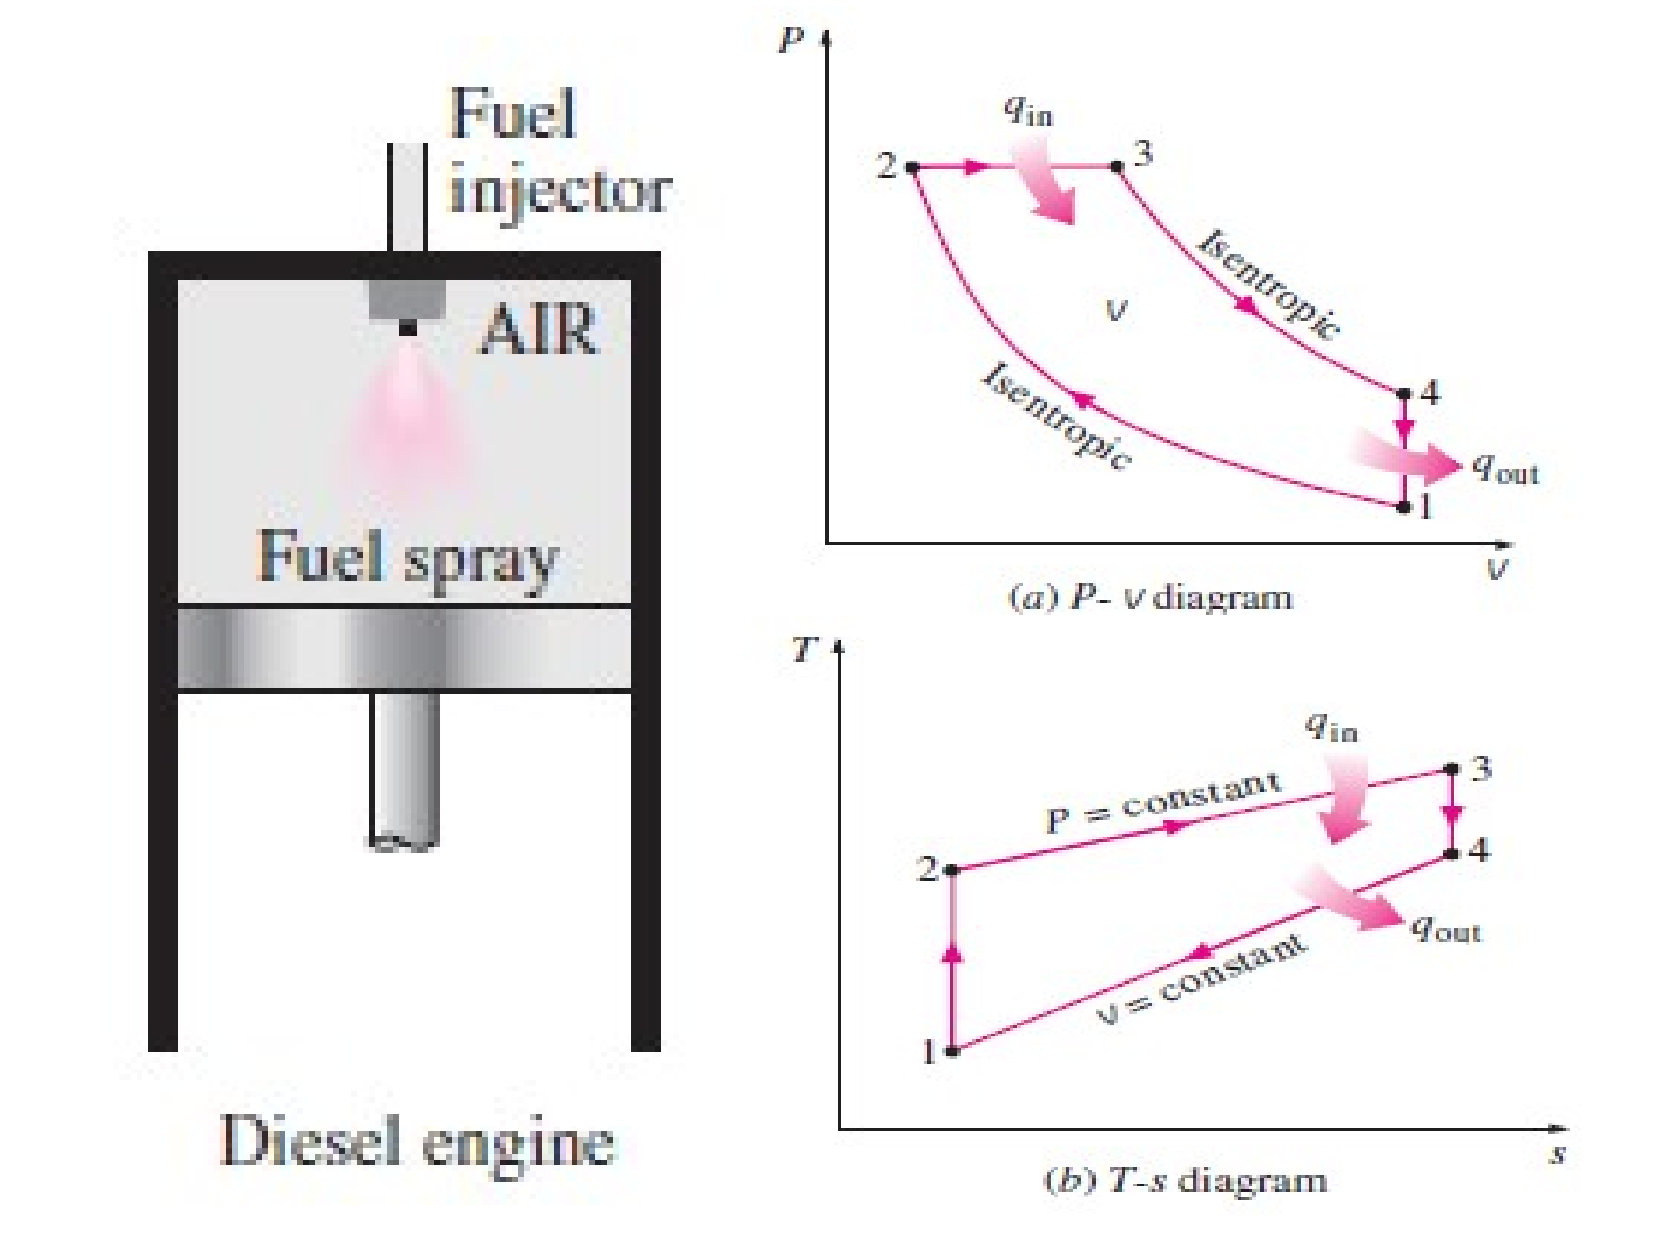
\includegraphics[width=6.cm,clip]{./Pics/InternalCombustion_IdealDieselCycle}
     \end{center}
    \end{figure}   
   \end{column}  
  \end{columns}
\end{frame}

%%%
%%% Slide
%%%
\begin{frame}
 \frametitle{Ideal Diesel Cycles}
  \begin{columns}
   \begin{column}[c]{0.5\linewidth}
    \begin{itemize}
     \item <1-> \textcolor{blue}{1--2} isentropic compression $\left(PV^{\gamma}=\text{ constant}\right)$: $\left(P_{1},V_{1},T_{1}\right)$ $\Rightarrow$ $\left(P_{2},V_{2},T_{2}\right)$;
     \item <2-> \textcolor{blue}{2--3} constant-pressure heat addition: $\left(P_{2},V_{2},T_{2}\right)$ $\Rightarrow$ $\left(P_{3}=P_{2},V_{3},T_{3}\right)$;
     \item <3-> \textcolor{red}{$3$} is called \textcolor{blue}{{\it point of cut-off}};
     \item <4-> \textcolor{blue}{3--4} isentropic expansion: $\left(P_{3},V_{3},T_{3}\right)$ $\Rightarrow$ $\left(P_{4},V_{4},T_{4}\right)$;
     \item <5-> \textcolor{blue}{4--1} constant-volume heat rejection: $\left(P_{4},V_{4},T_{4}\right)$ $\Rightarrow$ $\left(P_{1},V_{1}=V_{4},T_{4}\right)$.
    \end{itemize}
   \end{column}
   \begin{column}[c]{0.5\linewidth}
    \begin{figure}%
     \begin{center}
      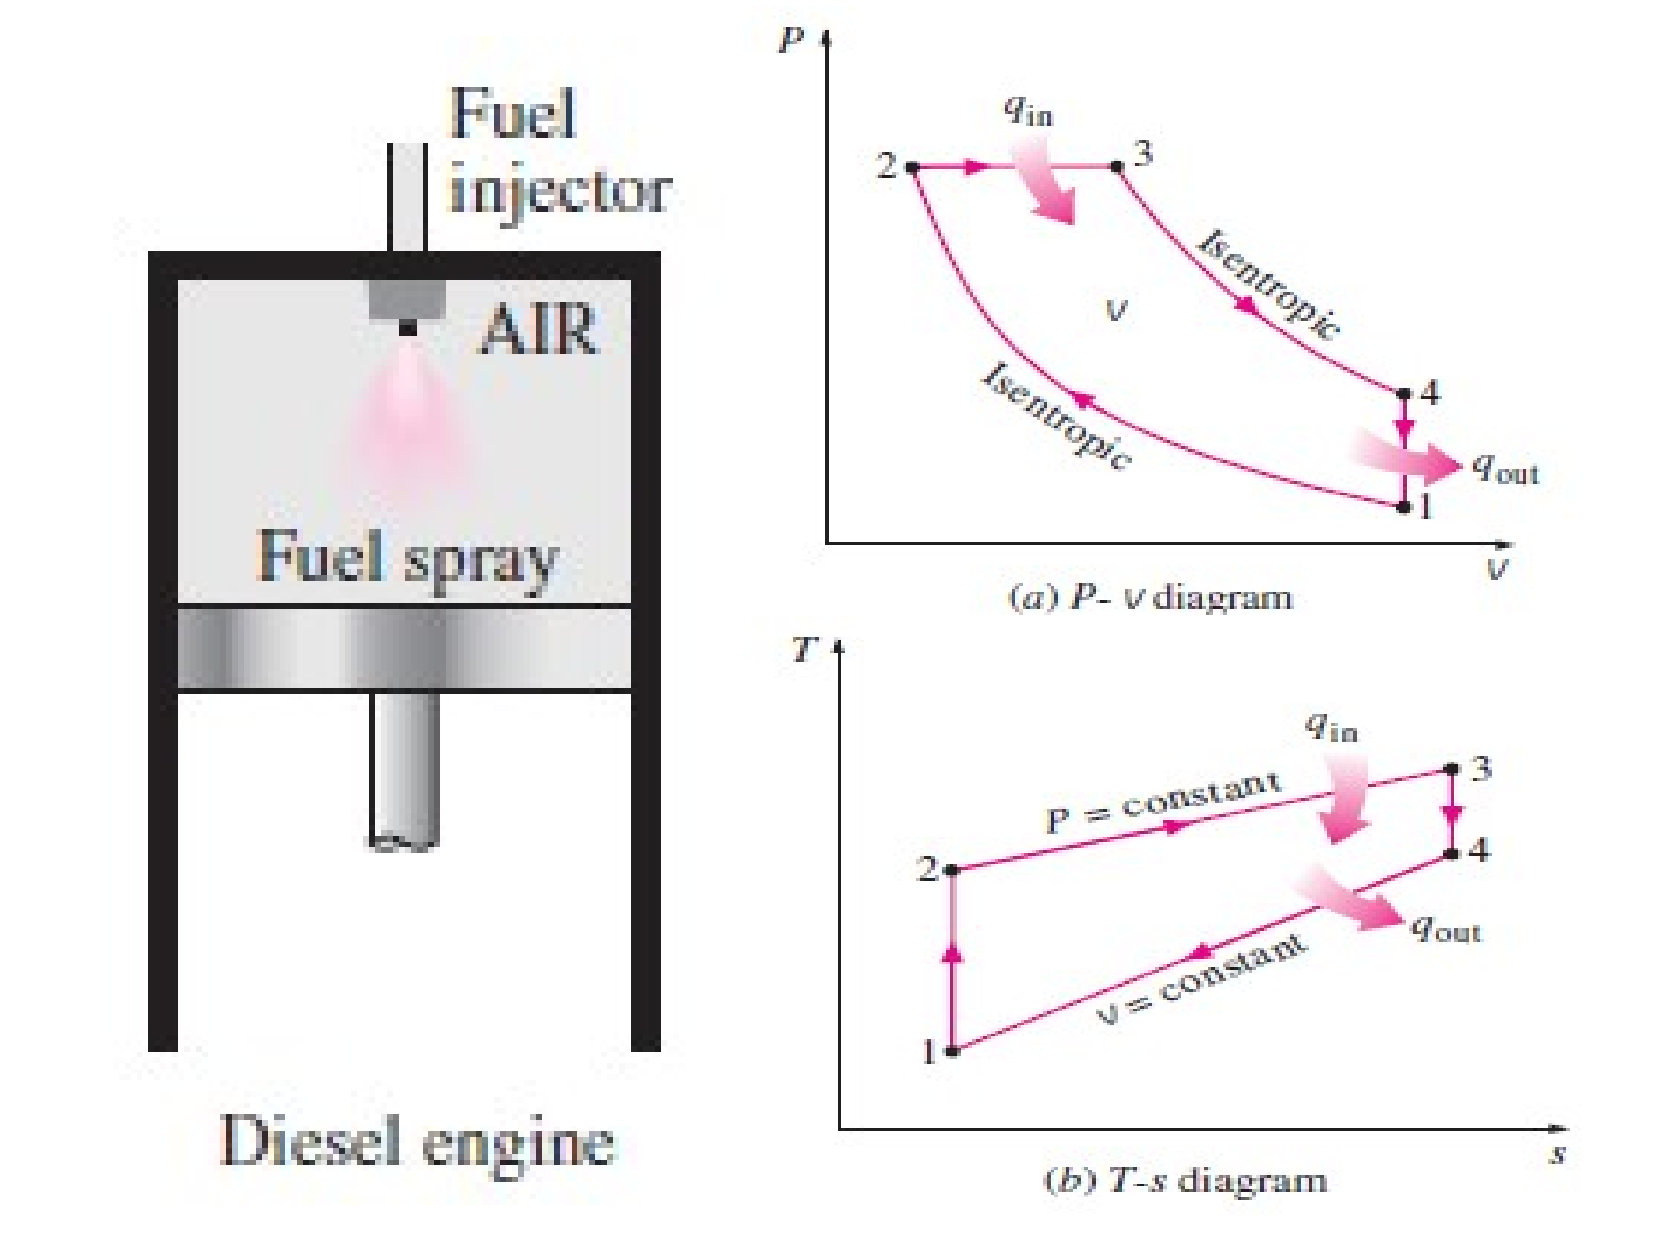
\includegraphics[width=6.cm,clip]{./Pics/InternalCombustion_IdealDieselCycle}
     \end{center}
    \end{figure}   
   \end{column}  
  \end{columns}
\end{frame}


%%%
%%% Slide
%%%
\begin{frame}
 \frametitle{{\it Pv} and {\it Ts} Diagrams: Ideal Otto and Diesel Cycles}
    \begin{figure}%
     \begin{center}
      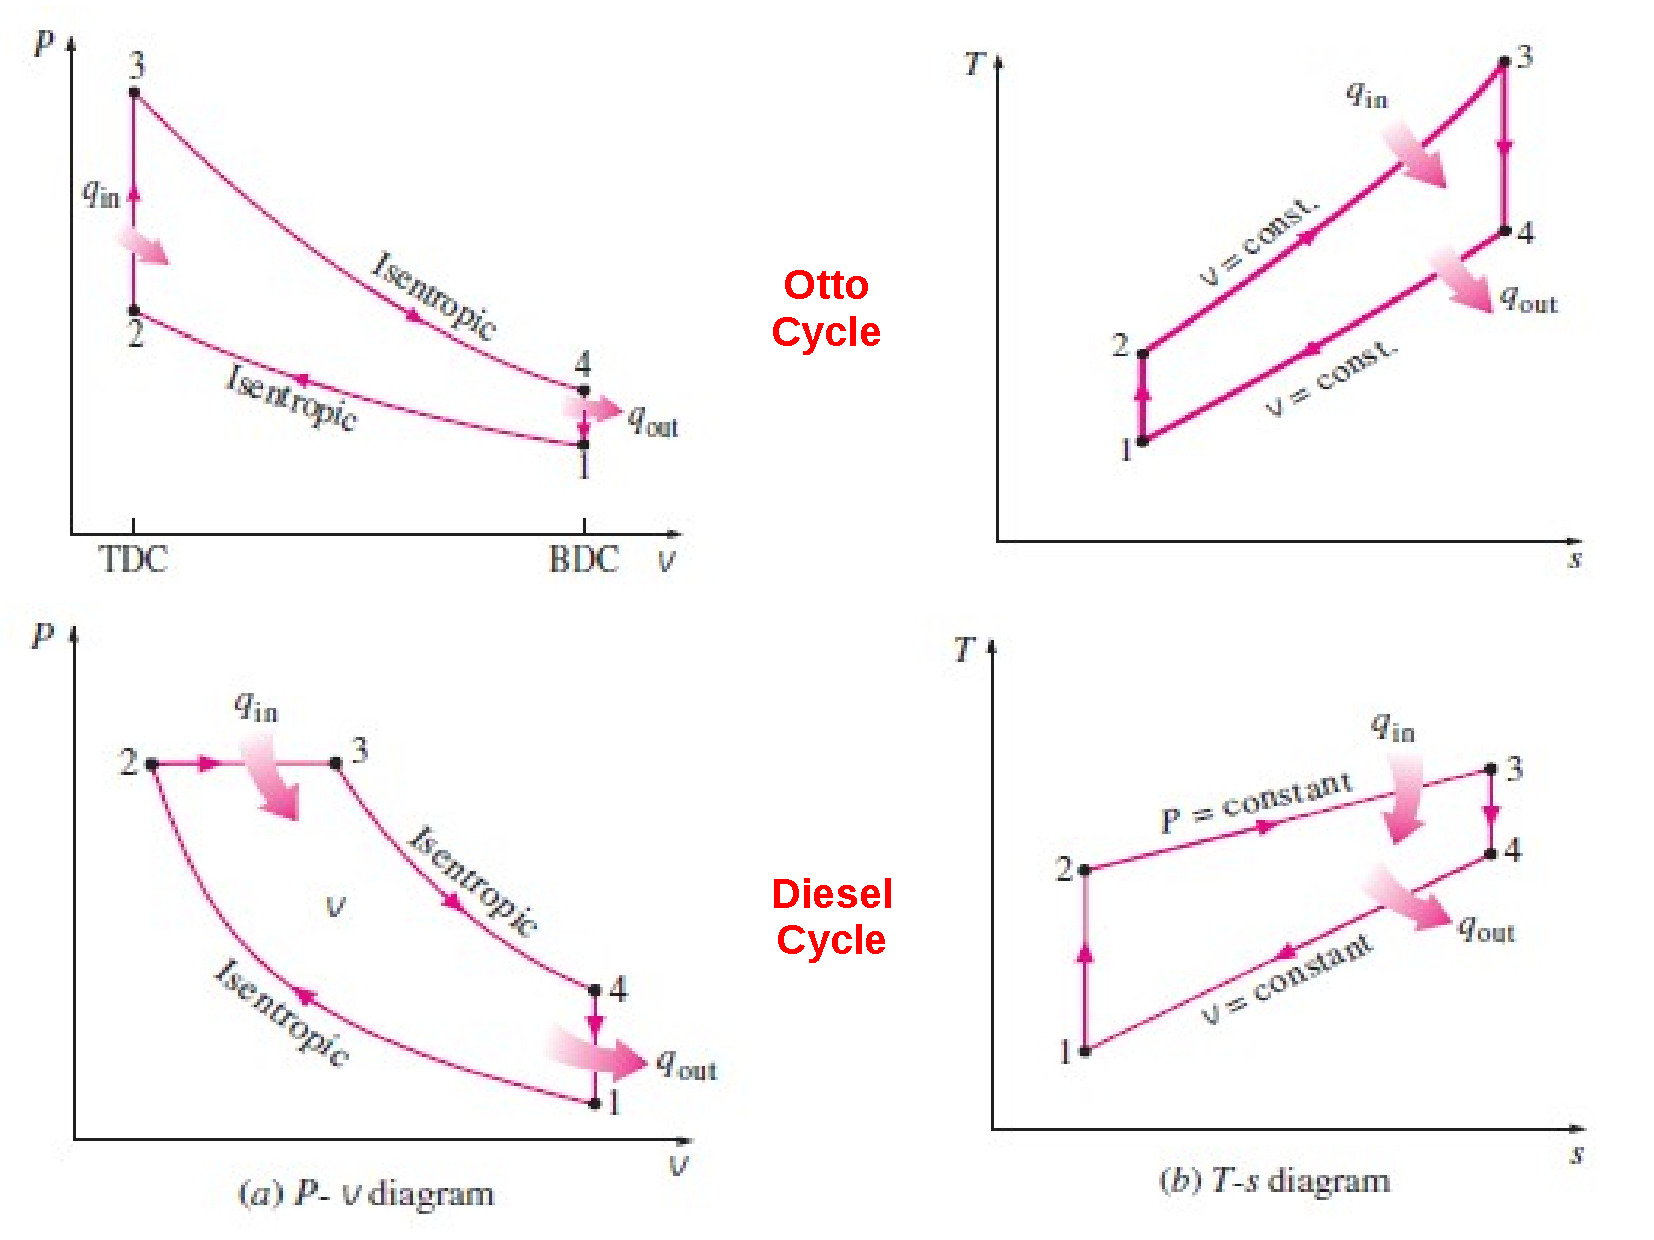
\includegraphics[width=10.cm,clip]{./Pics/InternalCombustion_IdealOttoxDieselCycles}
     \end{center}
    \end{figure}   
\end{frame}


%%%
%%% Slide
%%%
\begin{frame}
 \frametitle{Ideal Diesel Cycles -- Energy Balance:}
  \begin{columns}
   \begin{column}[c]{0.5\linewidth}
   Assuming 1 kg of air:
    \begin{itemize}
     \item <1-> Heat supplied at constant pressure: $Q_{s}=C_{p}\left(T_{3}-T_{2}\right)$;
     \item <2-> Heat rejected at constant volume: $Q_{r}=C_{v}\left(T_{4}-T_{1}\right)$;
     \item <3-> Work done: $W_{net}=C_{p}\left(T_{3}-T_{2}\right)-C_{v}\left(T_{4}-T_{1}\right)$.
    \end{itemize}
   \end{column}
   \begin{column}[c]{0.5\linewidth}
    %\begin{itemize}
    \begin{figure}%
     \begin{center}
      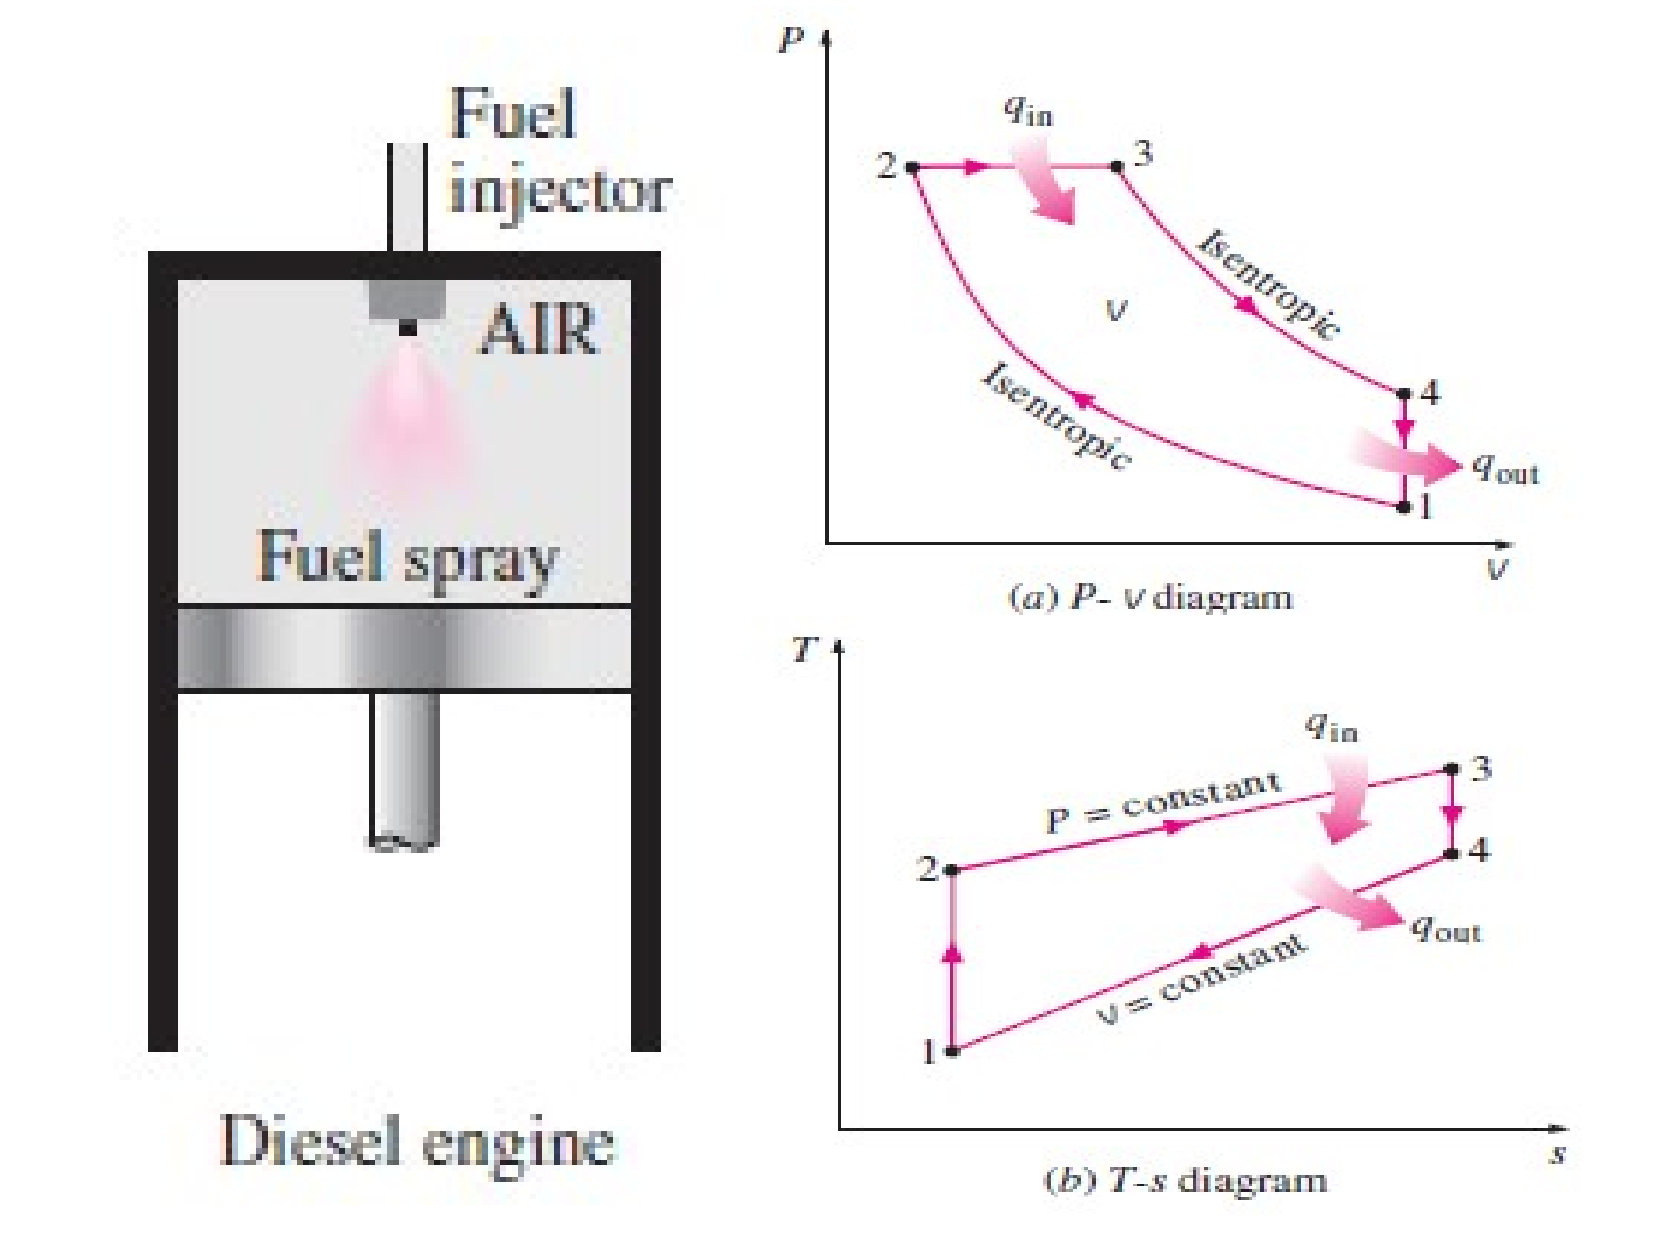
\includegraphics[width=6.cm,clip]{./Pics/InternalCombustion_IdealDieselCycle}
     \end{center}
    \end{figure}   
   \end{column}  
  \end{columns}
\end{frame}


%%%
%%% Slide
%%%
\begin{frame}
 \frametitle{Ideal Diesel Cycles -- Energy Balance:}
 \begin{itemize}
  \item <1-> Efficiency: 
   \begin{displaymath}
    \eta_{\text{Diesel}}=\displaystyle\frac{C_{p}\left(T_{3}-T_{2}\right)-C_{v}\left(T_{4}-T_{1}\right)}{C_{p}\left(T_{3}-T_{2}\right)} = 1 - \displaystyle\frac{T_{4}-T_{1}}{\gamma\left(T_{3}-T_{2}\right)}
   \end{displaymath}
  \item <2-> Assuming the compression ratio $\left(r\right)$ and cut-off ratio $\left(\rho\right)$:
   \begin{displaymath}
    r=\displaystyle\frac{V_{1}}{V_{2}}\;\;\;\text{ and }\;\;\;\rho=\displaystyle\frac{\text{volume at cut-off}}{\text{clearence volume}}=\displaystyle\frac{V_{3}}{V_{2}}
   \end{displaymath}
  \item <3-> Isentropic compression \textcolor{blue}{1--2}:
   \begin{displaymath}
    \displaystyle\frac{T_{2}}{T_{1}}=\left(\displaystyle\frac{V_{1}}{V_{2}}\right)^{\gamma-1}=r^{\gamma-1} \Rightarrow T_{2}=T_{1}r^{\gamma-1}
   \end{displaymath}
  \item <4-> Constant Pressure heat addition \textcolor{blue}{2--3}: 
   \begin{displaymath}
    \displaystyle\frac{T_{3}}{T_{2}}=\displaystyle\frac{V_{3}}{V_{2}}=\rho \Rightarrow T_{3}=\rho T_{2}=\rho T_{1} r^{\gamma-1}
   \end{displaymath}
 \end{itemize}
\end{frame}

%%%
%%% Slide
%%%
\begin{frame}
 \frametitle{Ideal Diesel Cycles -- Energy Balance:}
 \begin{itemize}
  \item <1-> Isentropic expansion \textcolor{blue}{3--4}:
   \begin{displaymath}
    \displaystyle\frac{T_{3}}{T_{4}} = \left(\displaystyle\frac{V_{4}}{V_{3}}\right)^{\gamma-1} = \left(\displaystyle\frac{V_{1}}{V_{3}}\right)^{\gamma-1}  = \left(\displaystyle\frac{V_{1}}{V_{2}}\displaystyle\frac{V_{2}}{V_{3}}\right)^{\gamma-1}= \left(\displaystyle\frac{r}{\rho}\right)^{\gamma-1} \Longrightarrow \;\; T_{4} = T_{1}\rho^{\gamma}
   \end{displaymath}
  \item <2-> Replacing $T_{i}$ in the efficiency expression:
   \begin{displaymath}
    \textcolor{blue}{\eta_{\text{Diesel}}}= 1 - \displaystyle\frac{T_{4}-T_{1}}{\gamma\left(T_{3}-T_{2}\right)} = 1 - \displaystyle\frac{\rho^{\gamma}-1}{\gamma r^{\gamma-1}\left(\rho-1\right)} =  \textcolor{blue}{1 -\displaystyle\frac{1}{r^{\gamma-1}}\left[\displaystyle\frac{\rho^{\gamma}-1}{\gamma\left(\rho-1\right)}\right]}
   \end{displaymath}
  \item <3-> Remember that $\eta_{\text{Otto}} =1 - \displaystyle\frac{1}{r^{\gamma-1}}$. It is clear that (as $\rho>1$) the term in square-brackets is always greater than 1, therefore;
  \item <4-> \textcolor{blue}{$\eta_{\text{Otto}} > \eta_{\text{Diesel}}$} when both cycles operates on the same compression ratio;
  \item <5-> Cut-off ratio decreases  $\Rightarrow$ $\eta_{\text{Diesel}}$ increases and;
  \item <6-> If $\rho\to 1$ (using Calculus L'H\^opital rule) $\Rightarrow$ term in the square-bracket $\to$ 1 and $\eta_{\text{Otto}} = \eta_{\text{Diesel}}$. 
 \end{itemize}
\end{frame}


%%%
%%% Slide
%%%
\begin{frame}
 \frametitle{Ideal Diesel Cycles -- Energy Balance:}
 \begin{itemize}
  \item <1-> \textcolor{blue}{Net work} for diesel cycle can be define (as a function of $P$ and $V$) as,
    \begin{displaymath}
     W_{\text{net}} = \displaystyle\frac{P_{1}V_{1}r^{\gamma-1}\left[\gamma\left(\rho-1\right)-r^{1-\gamma}\left(\rho^{\gamma}-1\right)\right]}{\gamma-1}
    \end{displaymath}
  \item <2-> And the MEP can be expressed as
    \begin{displaymath}
     \textcolor{blue}{MEP = \displaystyle\frac{P_{1}r^{\gamma}\left[\gamma\left(\rho-1\right)-r^{1-\gamma}\left(\rho^{\gamma}-1\right)\right]}{\left(\gamma-1\right)\left(r-1\right)}}
    \end{displaymath}
 \end{itemize}
\end{frame}


%%%
%%% Slide
%%%
\begin{frame}
 \frametitle{Ideal Diesel Cycles -- Example:}
\textcolor{blue}{An engine with 200 mm cylinder diameter and 300 mm stroke works on ideal Diesel cycle. The initial pressure and temperature of air are 1 bar and 27$^{\text{o}}$C, repectively. The cut-off is 8$\%$ of the stroke. Calculate: (a) pressures and temperatures at all stages; (b) theoretical air-standard efficiency; (c) MEP; (d) power of the engine if the working cycles per minute are 380. Assume that the compression ratio ($r$) is 15 and working fluid is air.}

\medskip

\begin{tabular}{l l l}
Given:    &                  &            \\
          & Cylinder Diameter& $D = 2.0\times 10^{-1}\;m$  \\
          & Stroke length    & $L = 3.0\times 10^{-1}\;m$ \\
       %   & Clearence Volume & $V_{c} = 2.63\times 10^{-3}\;m^{3}$ \\
          & Initial Pressure & $P_{1}= 1\;bar$   \\
          & Initial Temperature & $T_{1}=300.15\;K$ \\
          & Maximum Pressure & $P_{3}=25\;bar$\\
          & Cut-off          & $\displaystyle\frac{8}{100}V_{s}$ \\
Calculate:&                  & \\
          & $P_{i}$ and $T_{i}$ & 1$\leq$i$\leq$4 \\
          & $\eta_{\text{Diesel}}$ & \\
          & MEP              & \\
          & Power            & \\
\end{tabular}

\end{frame}



%%%
%%% Slide
%%%
\begin{frame}
 \frametitle{Ideal Diesel Cycles --  Example}
  \begin{columns}
   \begin{column}[c]{0.6\linewidth}
    \begin{itemize}
     \item <1-> Calculating $V_{1}=V_{s}+V_{c}=V_{s}+\displaystyle\frac{V_{s}}{r-1}$ in which;
     \item <2-> $V_{s}=\displaystyle\frac{\pi}{4}D^{2}L=9.42\times 10^{-3}\;m^{3}$ and;
     \item <3-> $V_{1} = \displaystyle\frac{r}{r-1}V_{s}$=1.01$\times$10$^{-2}$m$^{3}$
     \item <4-> The mass of air in the cyclinder is obtained from the ideal gas equation:
      \begin{displaymath}
       P_{1}V_{1}=mRT_{1}\;\Rightarrow\; m= 1.17\times 10^{-2}\;\text{kg/cycle}
      \end{displaymath}
     \item <5-> Isentropic compression  1--2:
      \begin{eqnarray}
       &&\displaystyle\frac{P_{2}}{P_{1}}=\left(\displaystyle\frac{V_{1}}{V_{2}}\right)^{\gamma}=r^{\gamma} \nonumber \\
       && \textcolor{blue}{P_{2}=44.31\text{ bar}}\nonumber
      \end{eqnarray}
    \end{itemize}
   \end{column}
   \begin{column}[c]{0.4\linewidth}
    \begin{figure}%
     \begin{center}
      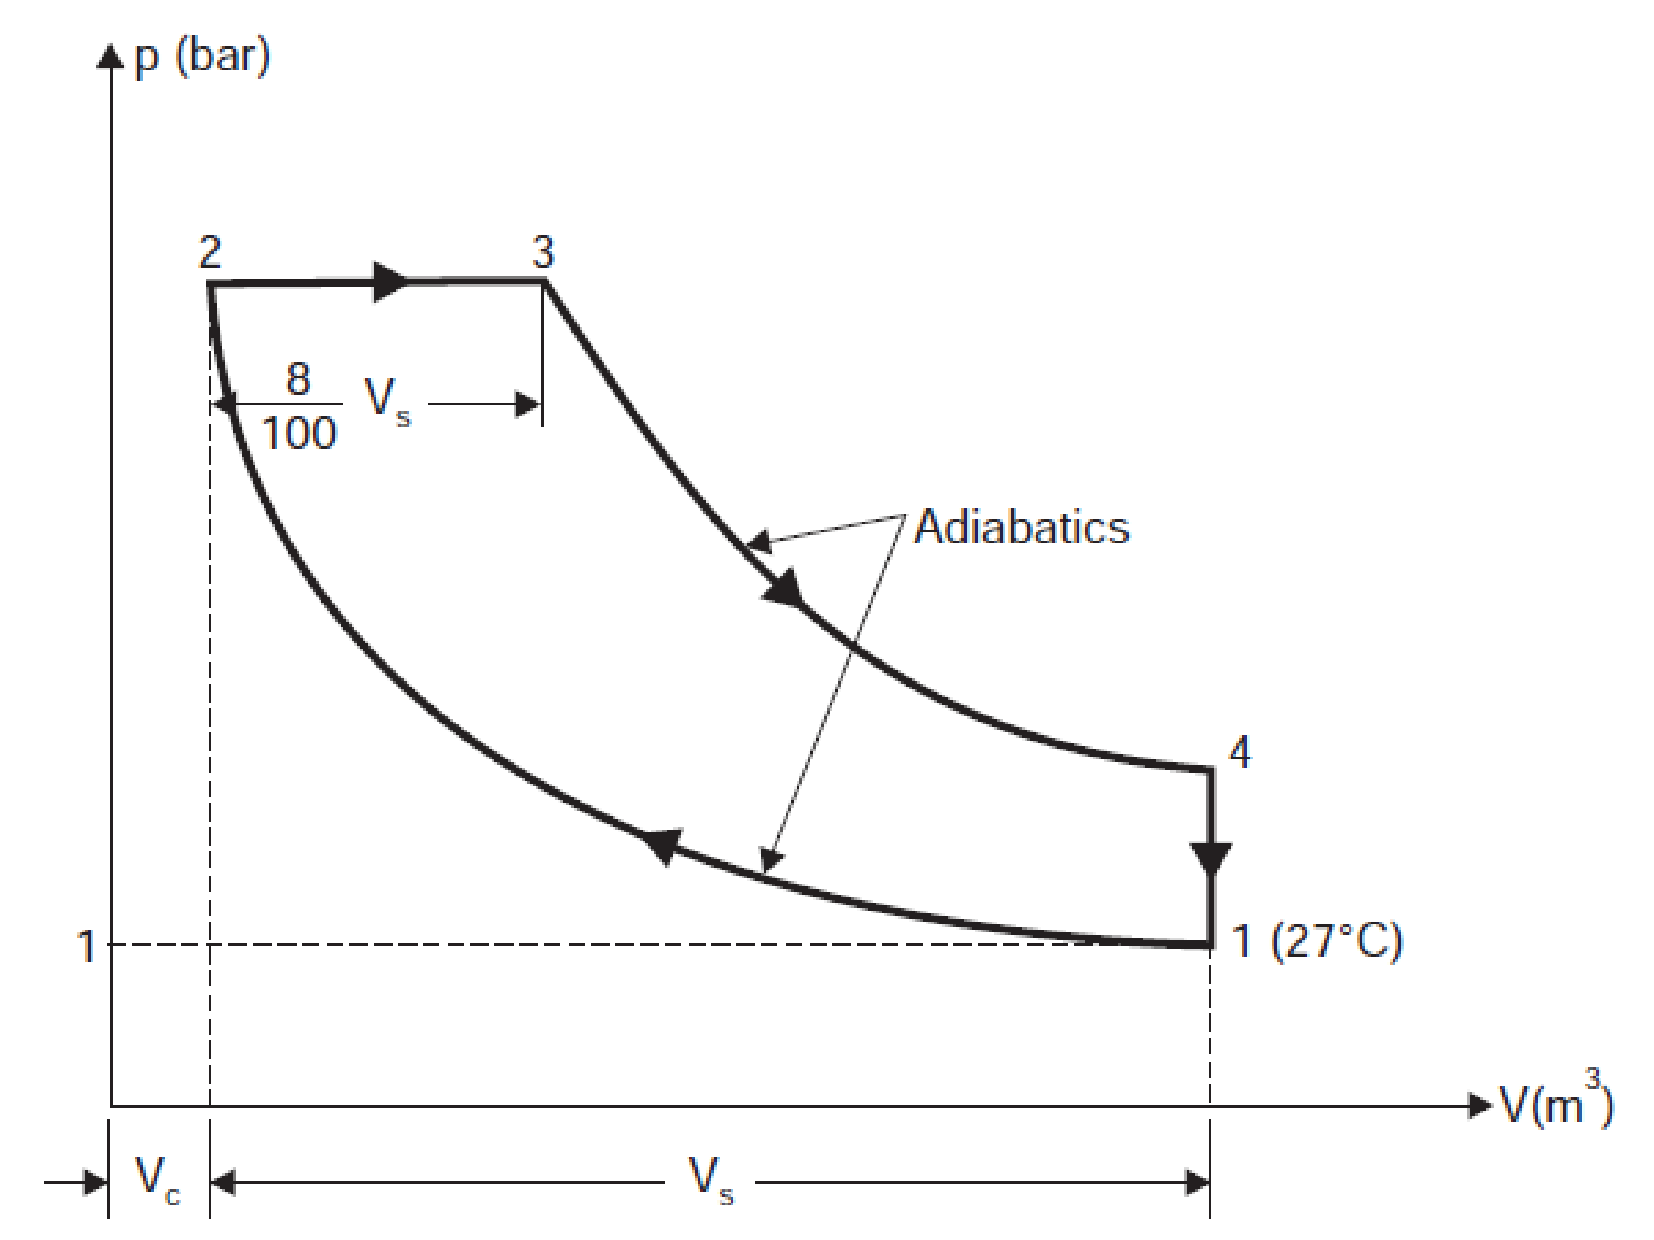
\includegraphics[width=5.cm,clip]{./Pics/InternalCombustion_IdealDieselCycle_Example1}
     \end{center}
    \end{figure}   
   \end{column}  
  \end{columns}
\end{frame}


%%%
%%% Slide
%%%
\begin{frame}
 \frametitle{Ideal Diesel Cycles --  Example}
    \begin{itemize}
     \item <1-> Isentropic compression  1--2:
      \begin{eqnarray}
       &&\displaystyle\frac{T_{2}}{T_{1}}=\left(\displaystyle\frac{V_{1}}{V_{2}}\right)^{\gamma-1}=r^{\gamma-1} \; \Rightarrow \;\textcolor{blue}{T_{2}=886.2\text{ K}}\nonumber \\
       && \textcolor{blue}{V_{2}}=V_{c}=\displaystyle\frac{V_{s}}{r-1}=\textcolor{blue}{6.728\times 10^{-4}\text{ m}^{3}} \nonumber
      \end{eqnarray}
     \item <2-> the \textcolor{red}{cut-off ratio} = 0.08 $=\displaystyle\frac{\rho-1}{r-1}$ $\Rightarrow$ $\rho= 2.12$;
     \item <3-> And $\textcolor{blue}{V_{3}}=\rho V_{2}=\textcolor{blue}{1.426\times 10^{-3}\text{ m}^{3}}$. The expansion at constant pressure 2--3:
       \begin{displaymath}
        \displaystyle\frac{V_{3}}{T_{3}} = \displaystyle\frac{V_{2}}{T_{2}} \Rightarrow \textcolor{blue}{T_{3}=1878.3\text{ K}= 1600.15^{\text{ o}}\text{C}}
       \end{displaymath}
     \item <4-> Isentropic expansion 3--4:
       \begin{eqnarray}
         && P_{3}V_{3}^{\gamma}=P_{4}V_{4}^{\gamma} \; \Rightarrow \; P_{4}=P_{3}\left(\displaystyle\frac{V_{3}}{V_{4}}\right)^{\gamma} \nonumber \\
         && \text{but as } \displaystyle\frac{V_{4}}{V_{3}} = \displaystyle\frac{V_{4}}{V_{2}} \displaystyle\frac{V_{2}}{V_{3}}= \displaystyle\frac{r}{\rho} \;\Rightarrow\; \textcolor{blue}{V_{4}=V_{1}=7.07\text{ m}^{3}} \nonumber \\
         && \textcolor{blue}{P_{4}=2.866\text{ bar}} \nonumber
       \end{eqnarray}
    \end{itemize}
\end{frame}


%%%
%%% Slide
%%%
\begin{frame}
 \frametitle{Ideal Diesel Cycles --  Example}
    \begin{itemize}
     \item <1-> And,
      \begin{eqnarray}
       && \displaystyle\frac{T_{4}}{T_{3}}=\left(\displaystyle\frac{V_{3}}{V_{4}}\right)^{\gamma-1}\;\Rightarrow\; \textcolor{blue}{T_{4}=858.38\text{ K}=585.23^{\text{ o}}\text{C}} \nonumber \\
       && \textcolor{blue}{V_{4}=V_{1}=1.01\times 10^{-2}\text{ m}^{3}}\nonumber
      \end{eqnarray}
     \item<2-> The air-standard efficiency of the Diesel cycle is
       \begin{displaymath}
        \textcolor{blue}{\eta_{\text{Diesel}}}= 1 -\displaystyle\frac{1}{r^{\gamma-1}}\left[\displaystyle\frac{\rho^{\gamma}-1}{\gamma\left(\rho-1\right)}\right] = \textcolor{blue}{0.598}
       \end{displaymath}        
     \item <3-> The mean effective pressure is
      \begin{displaymath}
       \textcolor{blue}{MEP} = \displaystyle\frac{P_{1}r^{\gamma}\left[\gamma\left(\rho-1\right)-r^{1-\gamma}\left(\rho^{\gamma}-1\right)\right]}{\left(\gamma-1\right)\left(r-1\right)} = \textcolor{blue}{7.424\text{ bar}}
      \end{displaymath}
     \item <4-> And the power $\left(\mathcal{P}\right)$ of the engine is given by
      \begin{eqnarray}
       \textcolor{blue}{\mathcal{P}}&=&\text{Work done per second} \nonumber \\
                                    &=& \text{Work done per cycle} \times \text{number of cycles per second} \nonumber \\
       &=& \left( MEP \times V_{s} \right) \times \displaystyle\frac{380}{60} = \textcolor{blue}{44.27\text{ kW}} \nonumber
      \end{eqnarray}
    \end{itemize}
\end{frame}


\subsection{Dual Combustion Cycle}
%%%
%%% Slide
%%%
\begin{frame}
 \frametitle{Dual Combustion Cycle}
  \begin{columns}
   \begin{column}[c]{0.45\linewidth}
    \begin{itemize}
     \item <1-> This cycle is also known as \textcolor{blue}{limited pressure or mixed cycle};
     \item <2-> Combination of \textcolor{blue}{Otto and Diesel} thermal cycles;
     \item <3-> Part of the heat is added at constant volume and;
     \item <4-> Other part of the heat is added at constant pressure --  thus;
     \item <5-> More time is available for the combustion of the fuel;
     \item <6-> Such time-lag combustion characteristic make this cycle better to be used for Diesel and hot spot ignition engines. 
    \end{itemize}
   \end{column}
   \begin{column}[c]{0.55\linewidth}
    \begin{figure}%
     \begin{center}
      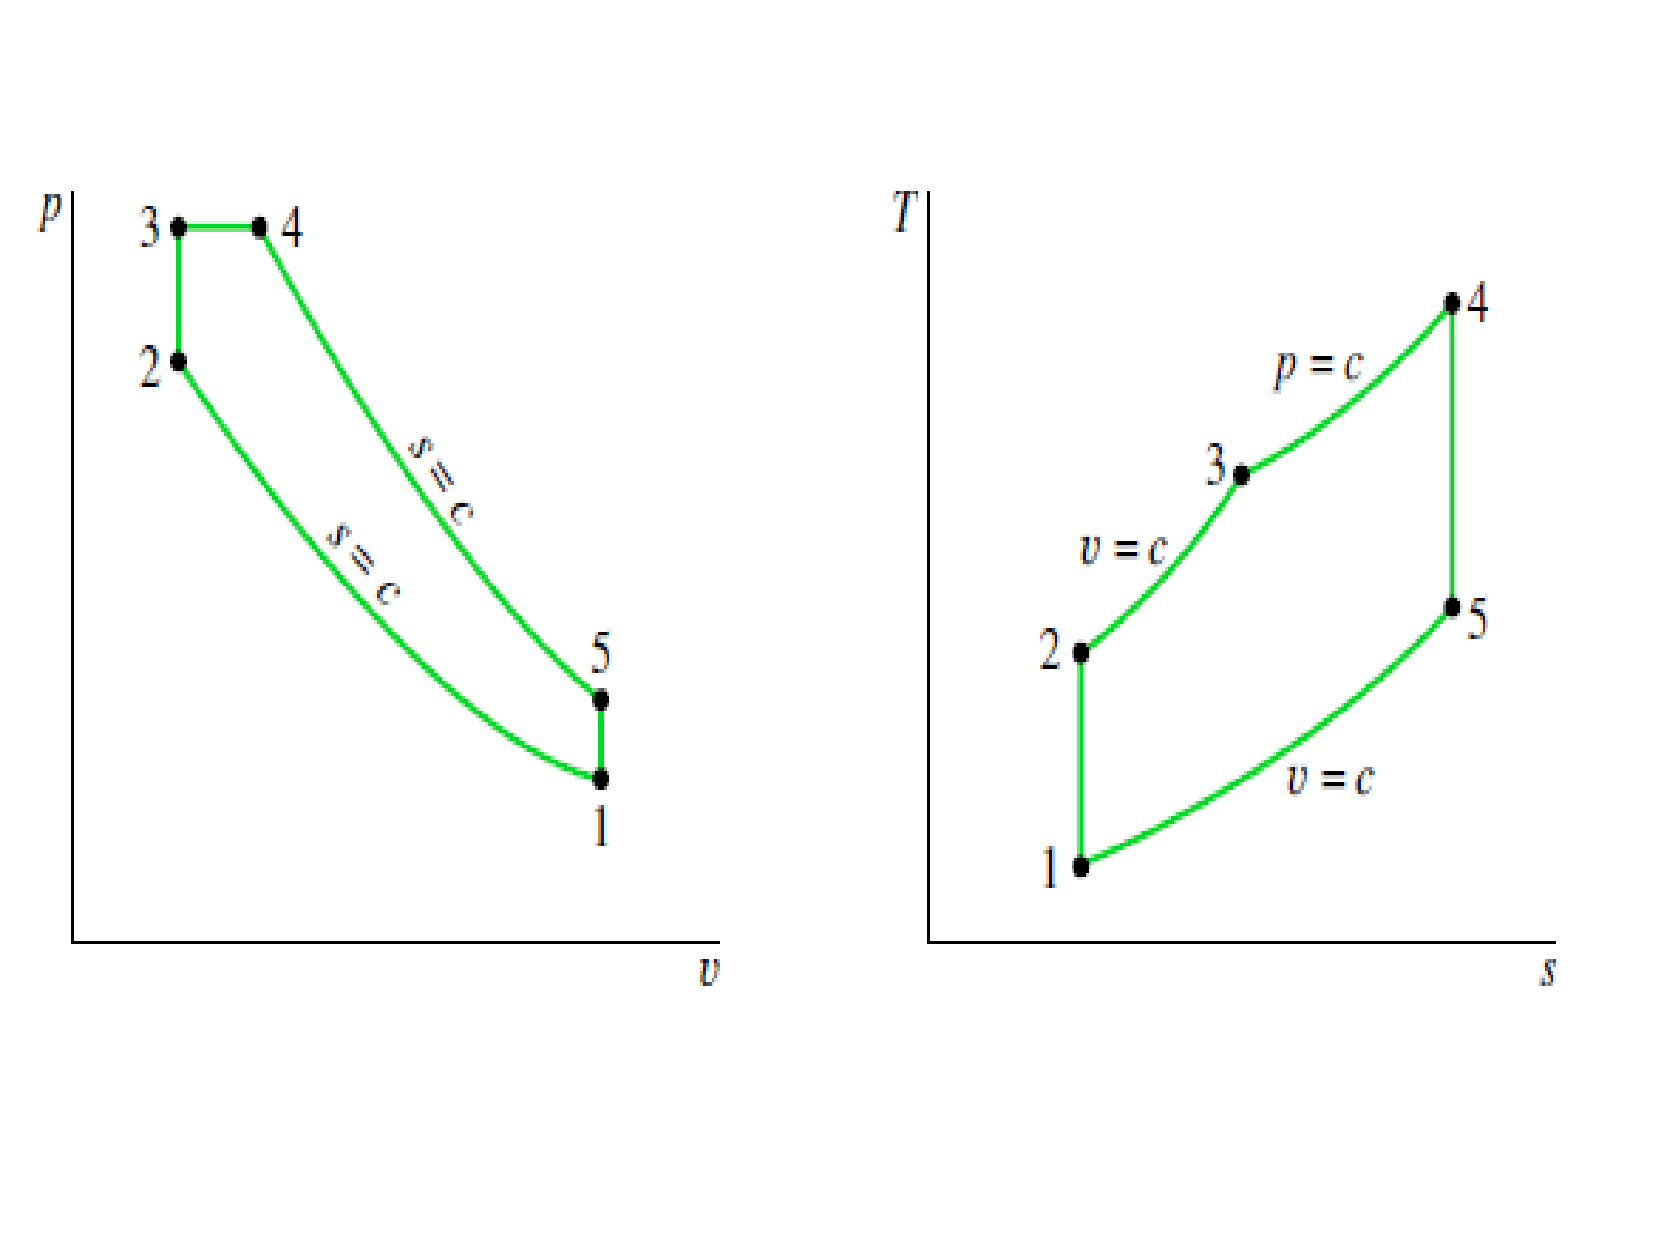
\includegraphics[width=6.cm,clip]{./Pics/InternalCombustion_IdealDualCombustion}
     \end{center}
    \end{figure}   
   \end{column}  
  \end{columns}
\end{frame}


%%%
%%% Slide
%%%
\begin{frame}
 \frametitle{Dual Combustion Cycle}
  \begin{columns}
   \begin{column}[c]{0.45\linewidth}
    \begin{itemize}
     \item <1-> \textcolor{blue}{1--2:} Isentropic compression;
     \item <2-> \textcolor{blue}{2--3:} Addition of heat at constant volume;
     \item <3-> \textcolor{blue}{3--4:} Addition of heat at constant pressure;
     \item <4-> \textcolor{blue}{4--5:} Isentropic expansion and;
     \item <5-> \textcolor{blue}{5--1:} Rejection of heat at constant volume.
    \end{itemize}
   \end{column}
   \begin{column}[c]{0.55\linewidth}
    \begin{figure}%
     \begin{center}
      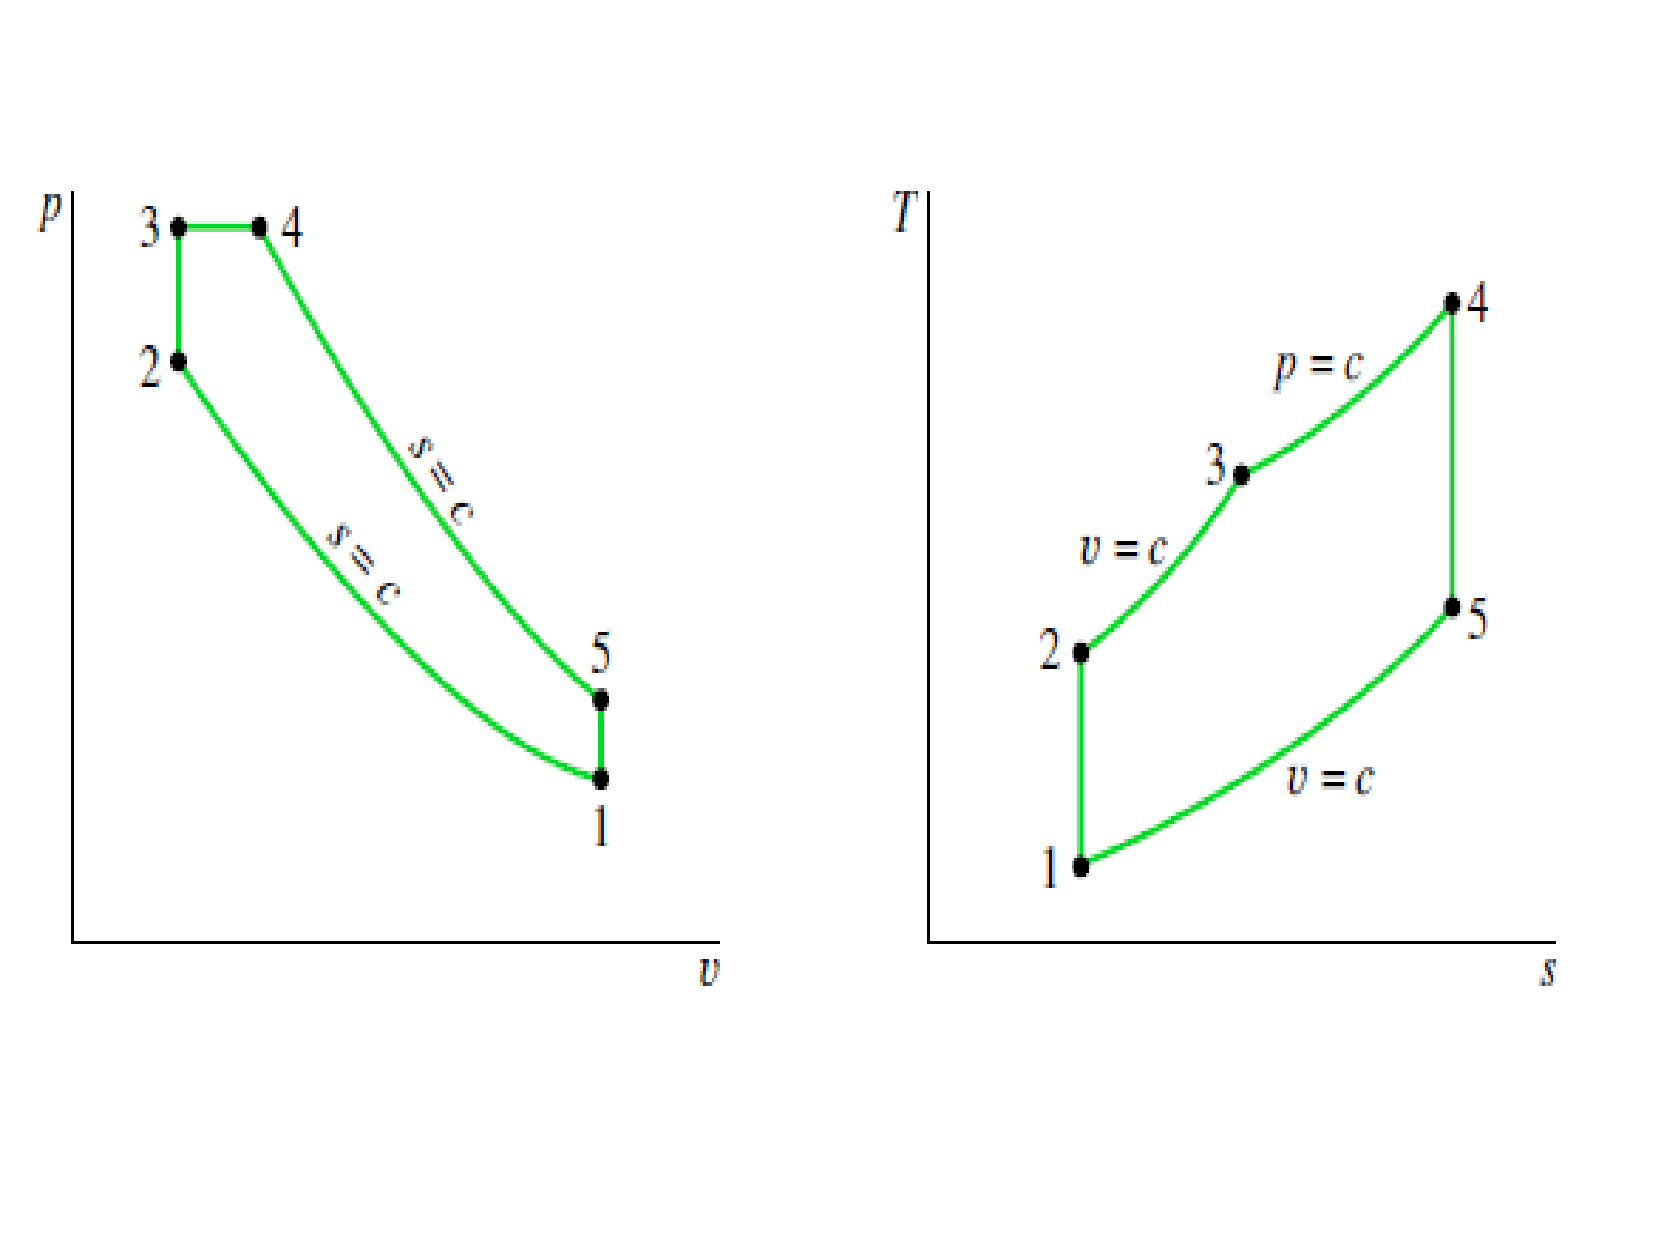
\includegraphics[width=6.cm,clip]{./Pics/InternalCombustion_IdealDualCombustion}
     \end{center}
    \end{figure}   
   \end{column}  
  \end{columns}
\end{frame}


%%%
%%% Slide
%%%
\begin{frame}
 \frametitle{Dual Combustion Cycle --  Thermal Analysis}
   Assuming 1 kg of air: 
    \begin{itemize}
     \item <1-> Total heat supplied (2--3 + 3--4): 
      \begin{displaymath}
       C_{v}\left(T_{3}-T_{2}\right) + C_{p}\left(T_{4}-T_{3}\right)
      \end{displaymath}  
     \item <2-> Heat rejected (5--1): $C_{v}\left(T_{5}-T_{1}\right)$
     \item <3-> Net work: 
       \begin{displaymath}
         W_{\text{net}}= C_{v}\left(T_{3}-T_{2}\right) + C_{p}\left(T_{4}-T_{3}\right)-C_{v}\left(T_{5}-T_{1}\right)
        \end{displaymath}
     \item <4-> And the compression ratio, $r=\displaystyle\frac{V_{1}}{V_{2}}$
     \item <4-> Efficiency:
      \begin{displaymath}
       \textcolor{blue}{\eta_{\text{Dual}}=1- \displaystyle\frac{C_{v}\left(T_{5}-T_{1}\right)}{\left(T_{3}-T_{2}\right)+\gamma\left(T_{4}-T_{3}\right)}}
      \end{displaymath}
    \end{itemize}
\end{frame}



%%%
%%% Slide
%%%
\begin{frame}
 \frametitle{Dual Combustion Cycle --  Thermal Analysis}
   Assuming 1 kg of air: 
    \begin{itemize}
     \item <1-> During heating at constant volume:
      \begin{eqnarray}
        &&\displaystyle\frac{P_{3}}{T_{3}}=\displaystyle\frac{P_{2}}{T_{2}}\;\Rightarrow \beta=\displaystyle\frac{T_{3}}{T_{2}}=\displaystyle\frac{P_{3}}{P_{2}} \nonumber 
      \end{eqnarray}
     \item <2-> where \textcolor{blue}{$\beta$ is the pressure or explosion ratio}. And therefore $T_{2}=T_{3}/\beta$
     \item <3-> And:
      \begin{displaymath}
       \displaystyle\frac{T_{4}}{T_{5}}=\left(\displaystyle\frac{V_{5}}{V_{4}}\right)^{\gamma-1}=\left(\frc{r}{\rho}\right)^{\gamma-1}
      \end{displaymath}
     \item <4-> And the heating at constant pressure: \\
 $T_{4}=T_{3}\frc{V_{4}}{V_{3}}=T_{3}\rho$, $T_{5}=\rho T_{3}\left(\frc{\rho}{r}\right)^{\gamma-1}$ and $T_{1}=\frc{T_{3}}{\beta}\frc{1}{r^{\gamma-1}}$
     \item <5-> Replacing $T_{i}$ in the $\eta_{\text{Dual}}$ expression:
     \begin{displaymath}
      \textcolor{blue}{\eta_{\text{Dual}} = 1 - \frc{1}{r^{\gamma-1}}\frc{\beta \rho^{\gamma}-1}{\left[\left(\beta-1\right)+\beta\gamma\left(\rho-1\right)\right]}}
     \end{displaymath}
    \end{itemize}
\end{frame}


%%%
%%% Slide
%%%
\begin{frame}
 \frametitle{Dual Combustion Cycle --  Thermal Analysis}
    \begin{itemize}
     \item <1-> The net work can be rewritten (as a function of $P$ and $V$) as,
      \begin{displaymath}
       \textcolor{blue}{W_{\text{net}}= \frc{P_{1}V_{1}r^{\gamma-1}\left[\beta\gamma \left(\rho-1\right)+\left(\beta-1\right)-r^{\gamma-1}\left(\beta\rho^{\gamma}-1\right)\right]}{\gamma-1}}
      \end{displaymath}
      \item <2-> And the MEP,
       \begin{displaymath}
        \textcolor{blue}{MEP = \frc{P_{1} r^{\gamma}\left[\beta\left(\rho-1\right)+\left(\beta-1\right)-r^{1-\gamma}\left(\beta\rho^{\gamma}-1\right)\right]}{\left(\gamma-1\right)\left(r-1\right)}}
       \end{displaymath}
    \end{itemize}
\end{frame}



\subsection{Comparing Otto, Diesel and Dual Combustion Cycles}
%%%
%%% Slide
%%%
\begin{frame}
 \frametitle{{\it Efficiency} $\times$ {\it Compression Ratio}}
  \begin{columns}
   \begin{column}[c]{0.4\linewidth}
    \begin{itemize}
     \item <1-> Air standard efficiencies increase with the increase in the compression ratio;
     \item <2-> For a given compression ratio Otto cycle is the most efficient:
     \item <3-> \textcolor{blue}{$\eta_{\text{Otto}} \; > \; \eta_{\text{Dual}} \; > \; \eta_{\text{Diesel}}$}.
    \end{itemize}
   \end{column}
   \begin{column}[c]{0.6\linewidth}
    \begin{figure}%
     \begin{center}
      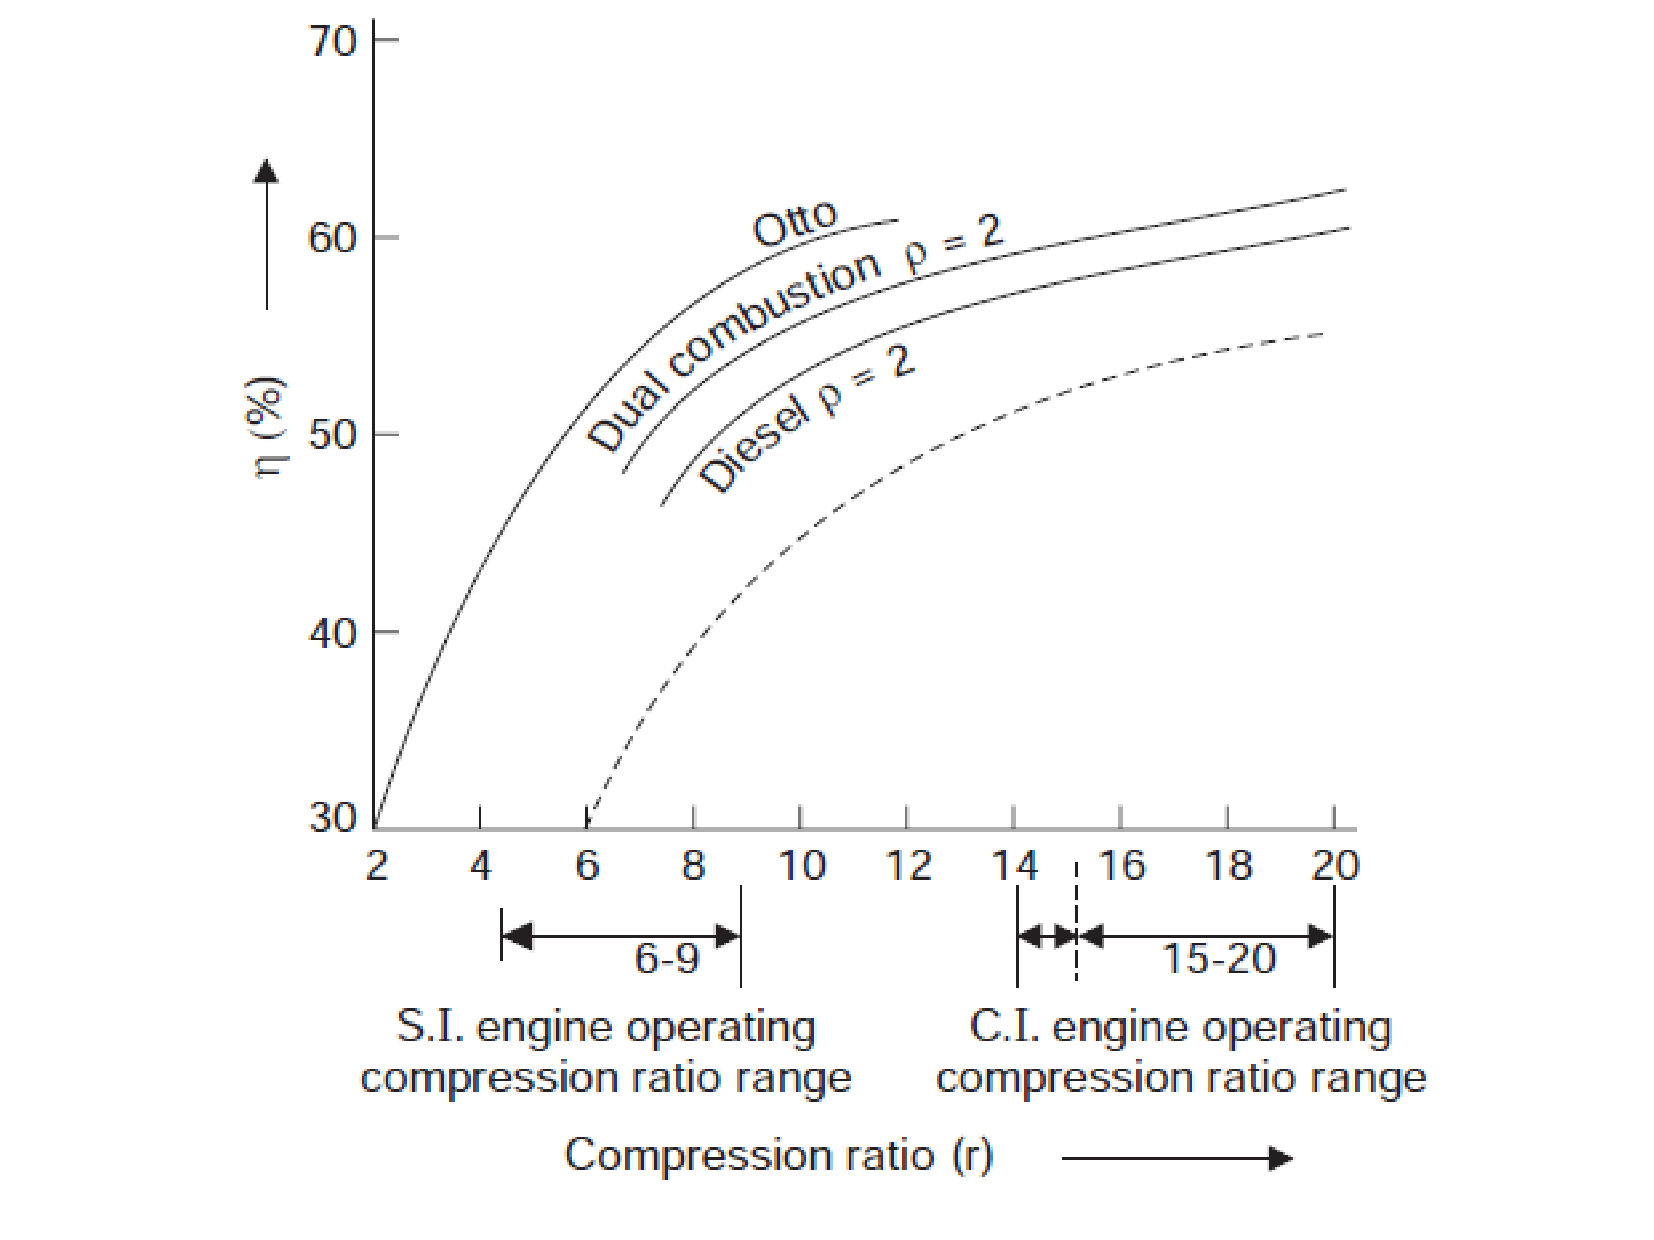
\includegraphics[width=7.cm,clip]{./Pics/InternalCombustion_Comparison1}
     \end{center}
    \end{figure}   
   \end{column}  
  \end{columns}
\end{frame}


%%%
%%% Slide
%%%
\begin{frame}
 \frametitle{Cycles at same Compression Ratio and Heat Input}
  \begin{columns}
   \begin{column}[c]{0.4\linewidth}
    \begin{itemize}
     \item <1-> As all cycles reject the heat at the same specific volume, the quantity of heat rejected from each cycle is represented by the appropriate area under the line \textcolor{blue}{4--1} on the $Ts$ diagram;
     \item <2-> From the original definition of efficiency,         
       \begin{displaymath}
        \eta = 1 - \frc{\text{heat rejected}}{\text{heat supplied}},
       \end{displaymath}
    \item <3-> the cycle which has the smaller heat rejected will have the highest efficiency. Thus, 
    \item <4-> \textcolor{blue}{$\eta_{\text{Otto}} \; > \; \eta_{\text{Dual}} \; > \; \eta_{\text{Diesel}}$}.
    \end{itemize}
   \end{column}
   \begin{column}[c]{0.6\linewidth}
    \begin{figure}%
     \begin{center}
      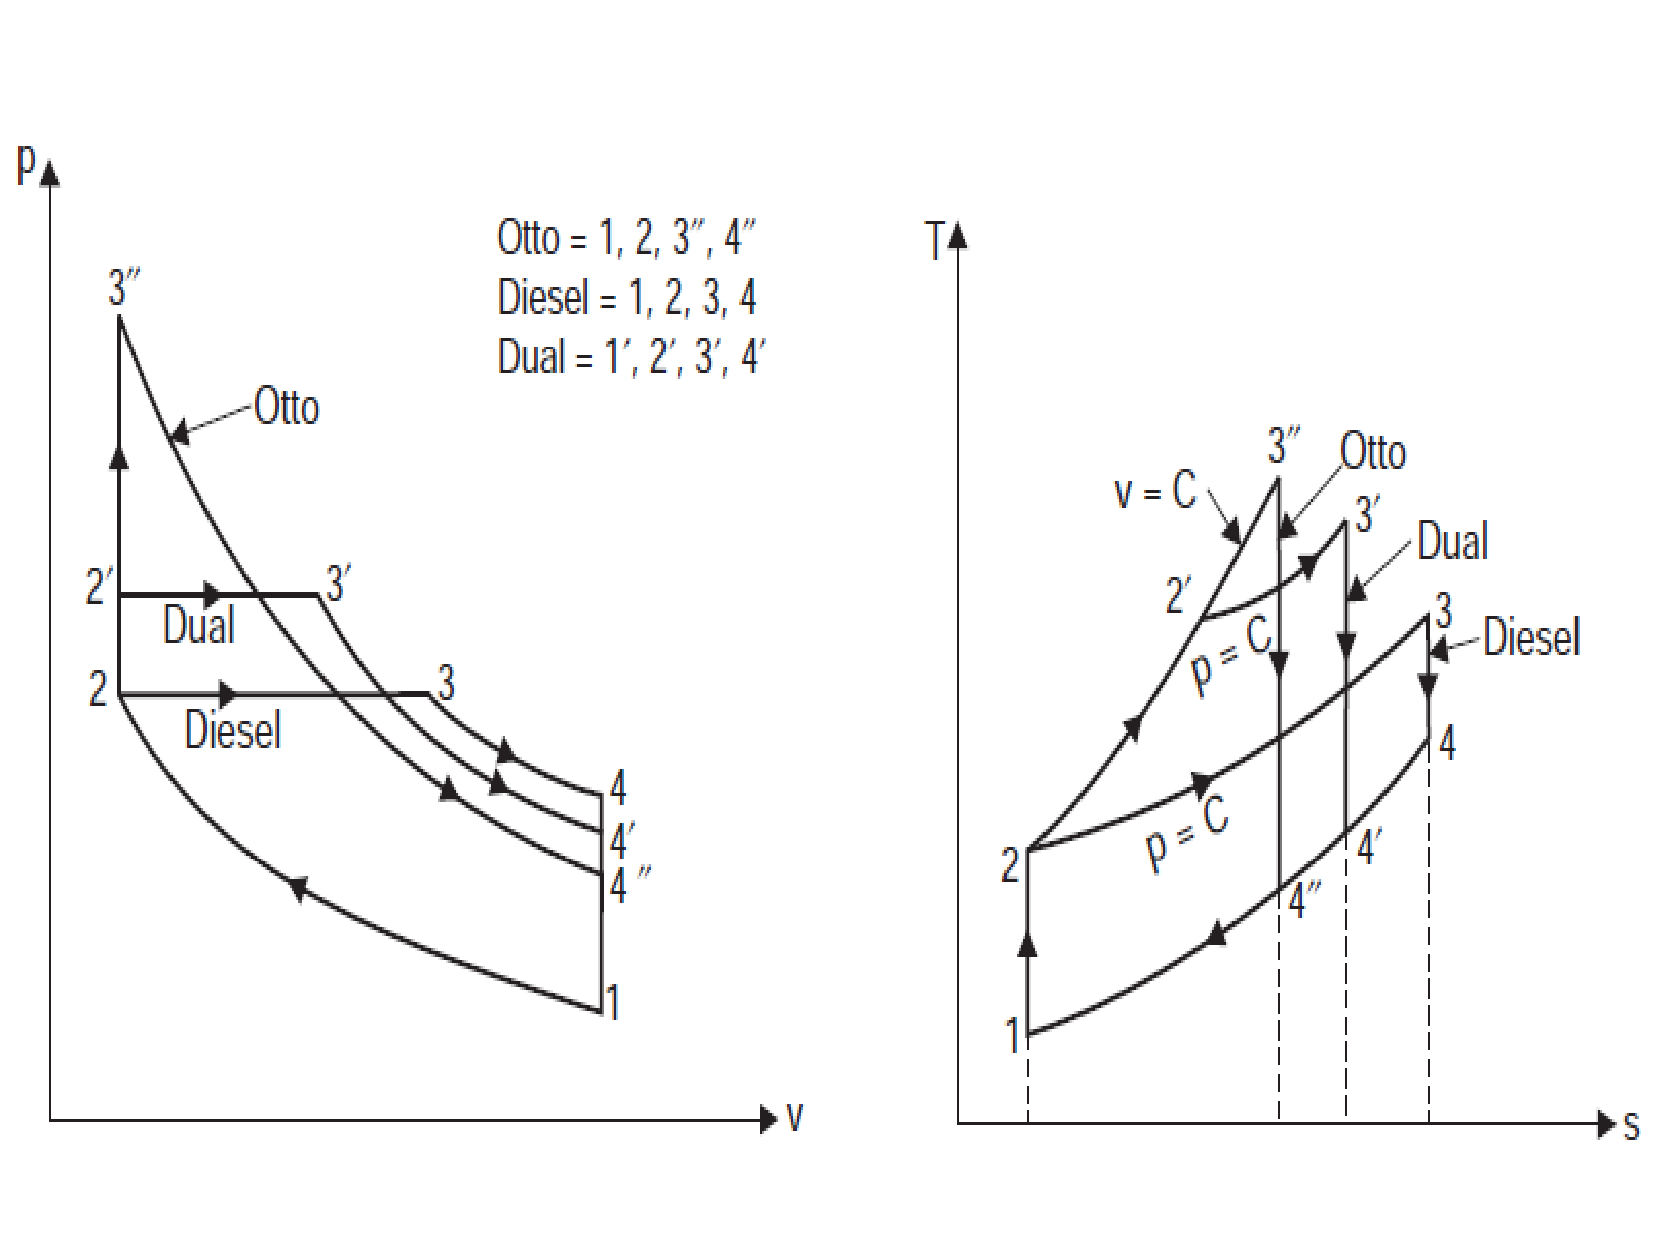
\includegraphics[width=7.cm,clip]{./Pics/InternalCombustion_Comparison2}
     \end{center}
    \end{figure}   
   \end{column}  
  \end{columns}
\end{frame}


%%%
%%% Slide
%%%
\begin{frame}
 \frametitle{Otto and Diesel Cycles at Constant Maximum Pressure and Heat Supplied}
  \begin{columns}
   \begin{column}[c]{0.4\linewidth}
    \begin{itemize}
     \item <1-> For maximum pressure, \textcolor{blue}{3} and \textcolor{blue}{3$^{\prime}$} must lie on a constant pressure line;
     \item <2-> On $Ts$ diagram, the heat rejected from the Diesel cycle is represented by the area under \textcolor{blue}{4--1} and;
     \item <3-> This area is smaller than the area from the Otto cycle -- \textcolor{blue}{4$^{\prime}$--1}, thus;
     \item <4-> Diesel cycles are more efficient than Otto cycles for the condition of maximum pressure and heat supplied.
    \end{itemize}
   \end{column}
   \begin{column}[c]{0.6\linewidth}
    \begin{figure}%
     \begin{center}
      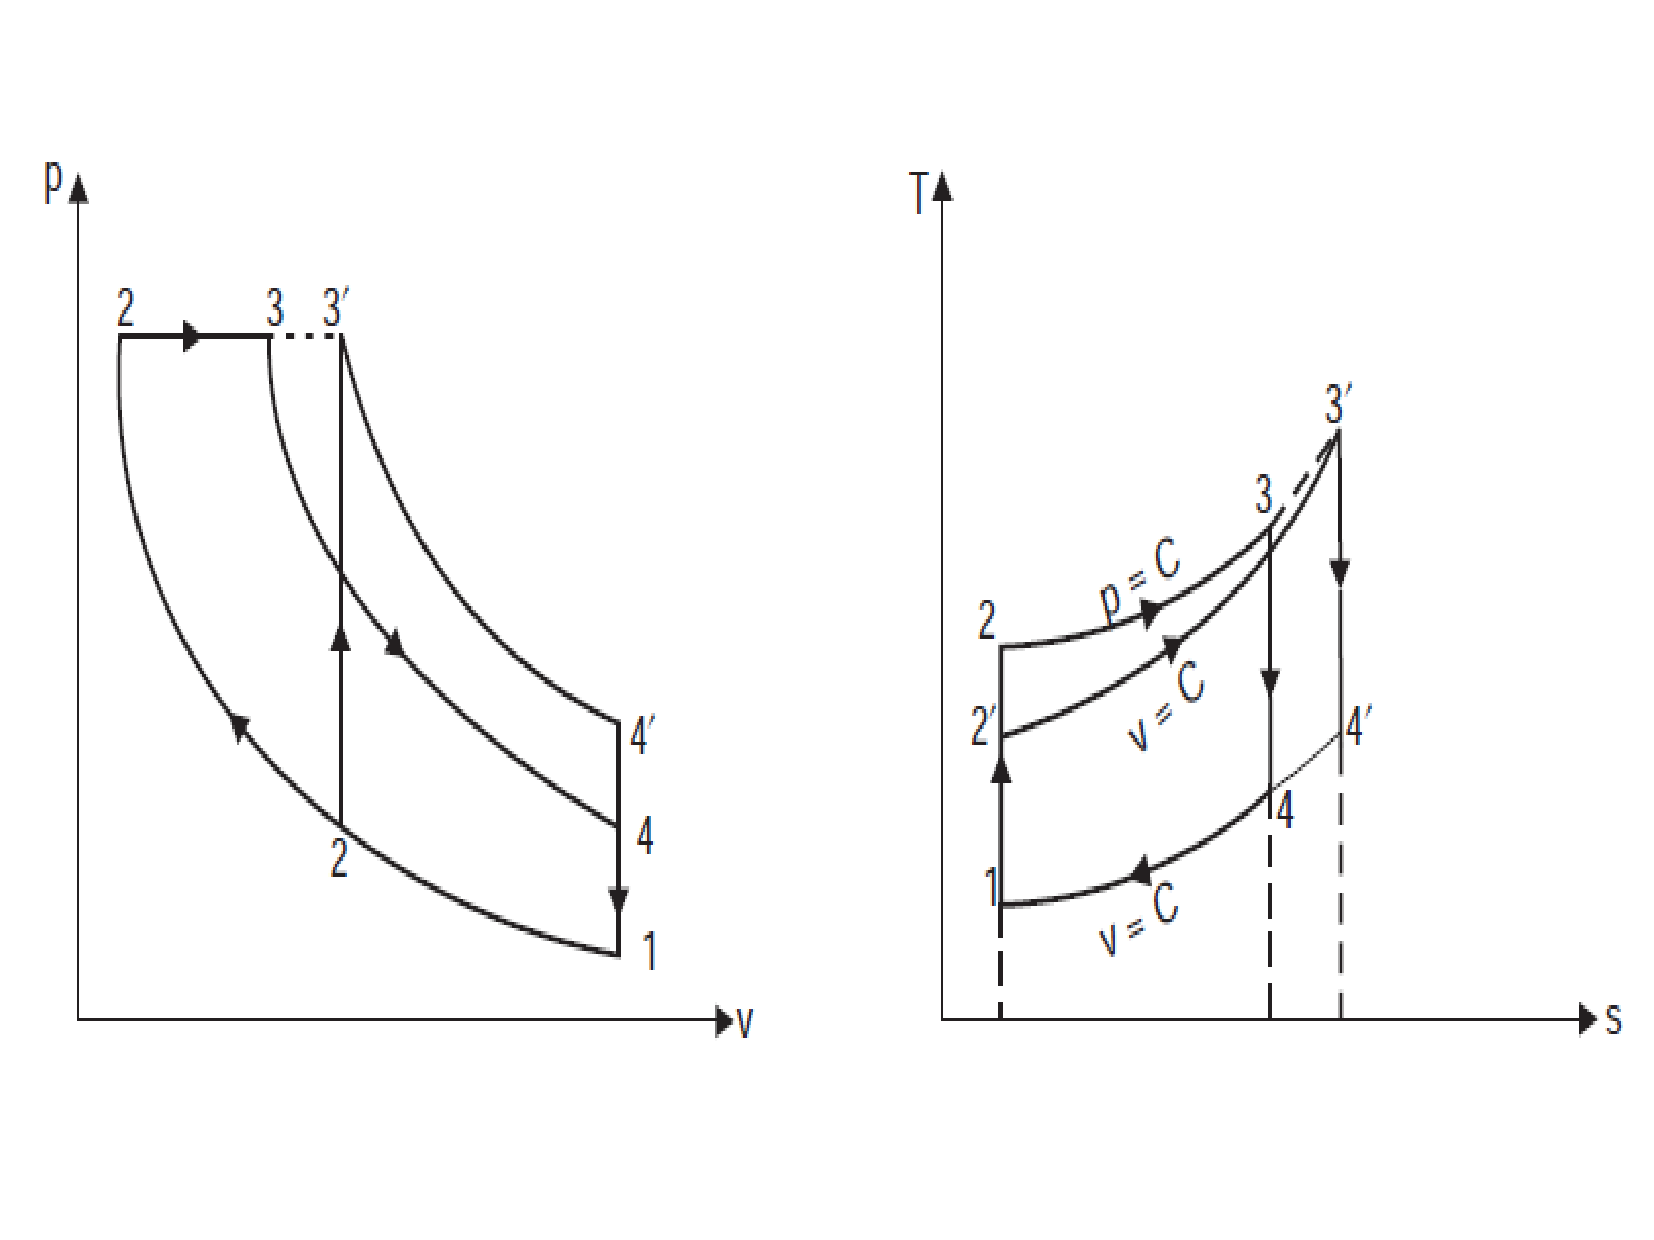
\includegraphics[width=7.cm,clip]{./Pics/InternalCombustion_Comparison3}
      \caption{Otto $\left(\text{1--2}^{\prime}\text{--3}^{\prime}\text{--4}^{\prime}\right)$ and Diesel (1--2--3--4) cycles.}
     \end{center}
    \end{figure}   
   \end{column}  
  \end{columns}
\end{frame}

\subsection{Atkinson Cycle}
%%%
%%% Slide
%%%
\begin{frame}
 \frametitle{Atkinson Cycle}
  \begin{columns}
   \begin{column}[c]{0.5\linewidth}
    \begin{itemize}
     \item <1-> \textcolor{blue}{1--2:} Heat rejection at constant pressure;
     \item <2-> \textcolor{blue}{2--3:} Adiabatic compression;
     \item <3-> \textcolor{blue}{3--4:} Addition of heat at constant volume and;
     \item <4-> \textcolor{blue}{4--1:} Adiabatic expansion. 
    \end{itemize}
   \end{column}
   \begin{column}[c]{0.5\linewidth}
    \begin{figure}%
     \begin{center}
      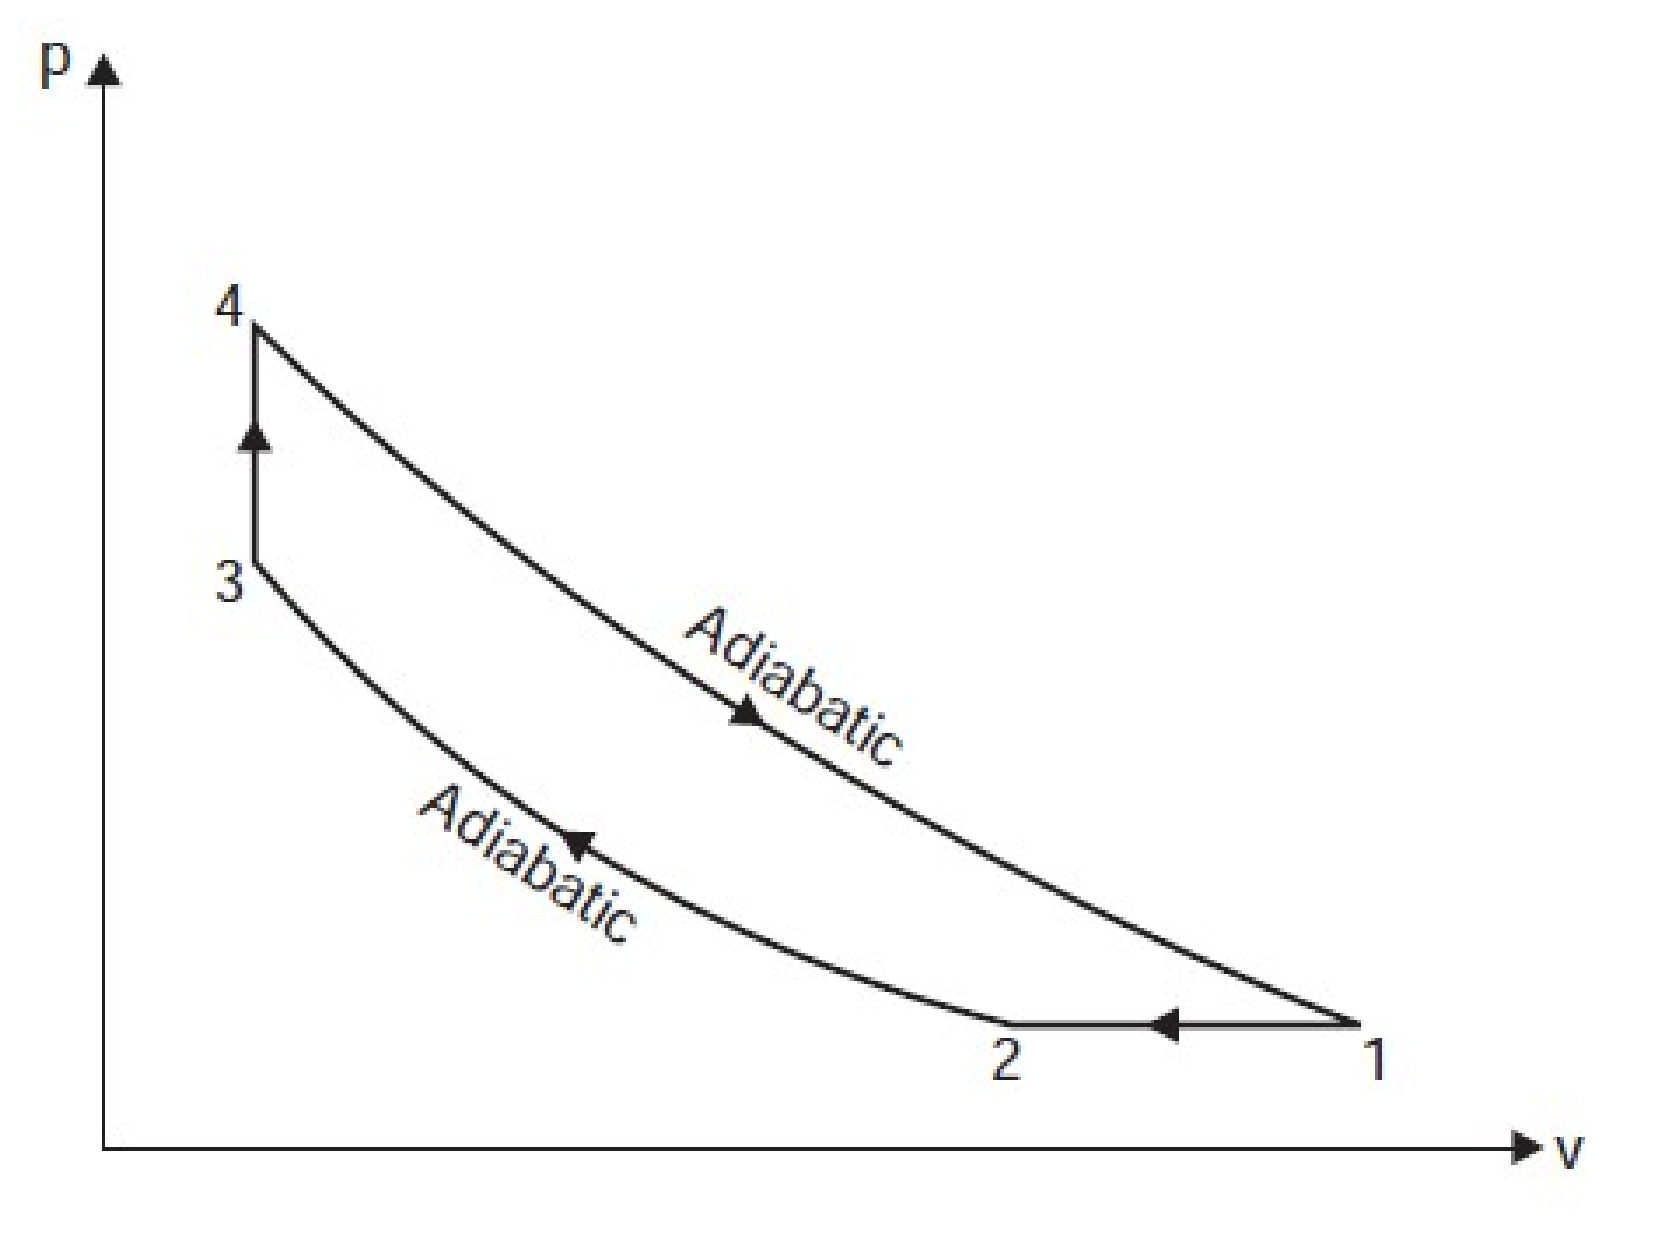
\includegraphics[width=6.cm,clip]{./Pics/InternalCombustion_IdealAtkinsonCombustion}
     \end{center}
    \end{figure}   
   \end{column}  
  \end{columns}
\end{frame}


%%%
%%% Slide
%%%
\begin{frame}
 \frametitle{Atkinson Cycle-- Thermal Analysis}
   Let's assume 1 kg of air in the cycle,
    \begin{itemize}
     \item <1-> \textcolor{blue}{Expansion ratio: } $r=\frc{V_{1}}{V_{4}}$
     \item <2-> \textcolor{blue}{Compression ratio:} $\alpha=\frc{V_{2}}{V_{3}}$
     \item <3-> \textcolor{blue}{Heat supplied at constant volume:} $C_{v}\left(T_{4}-T_{3}\right)$;
     \item <4-> \textcolor{blue}{Heat rejected:} $C_{p}\left(T_{1}-T_{2}\right)$;
     \item <5-> \textcolor{blue}{Net Work:} $C_{v}\left(T_{4}-T_{3}\right)-C_{p}\left(T_{1}-T_{2}\right)$;
     \item <6-> \textcolor{blue}{Efficiency:}
      \begin{displaymath}
       \eta_{\text{Atkinson}} = \frc{C_{v}\left(T_{4}-T_{3}\right)-C_{p}\left(T_{1}-T_{2}\right)}{C_{v}\left(T_{4}-T_{3}\right)}=1-\gamma\frc{T_{1}-T_{2}}{T_{4}-T_{3}}
      \end{displaymath}
    \item <7-> After the energy balances for each stroke (similar to the previous cycles) to calculate $P_{i}$ and $T_{i}$:
         \begin{displaymath}
         \textcolor{blue}{\eta_{\text{Atkinson}} = 1 - \gamma\left[\frc{r - \alpha}{r^{\gamma}-\alpha^{\gamma}}\right]}
         \end{displaymath}
    \end{itemize}
\end{frame}



\subsection{Stirling and Ericsson Cycles}
%%%
%%% Slide
%%%
\begin{frame}
 \frametitle{Stirling and Ericsson Cycles}
    \begin{itemize}
     \item <1-> Ideal Otto and Diesel cycles are composed of internally reversible processes and thus are internally reversible;
     \item <2-> However, they are not reversible as they involve heat transfer through a finite temperature difference during the non-isothermal heat-addition and heat-rejection processes (irreversible processes);
     \item <3-> If we imagine a heat engine that operates fully reversibly between a heat source, $T_{H}$, and a heat sink, $T_{L}$ then;
     \item <4-> The temperature difference between the working fluid and the heat source (or sink) can not exceed a differential amount $dT$ during any heat transfer process;
     \item <5-> In other words, both the heat-addition and heat-rejection processes during the cycle must occur isothermally: one at $T_{H}$ and the other at $T_{L}$;
     \item <6-> We saw this cycle as the intrinsic formulation of the \textcolor{blue}{Carnot cycle};
     \item <7-> \textcolor{blue}{Stirling and Ericsson cycles} involve isothermal heat-addition at $T_{H}$ and isothermal heat rejection at $T_{L}$. 
    \end{itemize}
\end{frame}


%%%
%%% Slide
%%%
\begin{frame}
 \frametitle{Stirling and Ericsson Cycles}
    \begin{itemize}
     \item <1-> In both cycles, the two isentropic processes are replaced by:
      \begin{enumerate}
       \item <2-> Stirling cycle: two constant-volume regeneration processes; 
       \item <3-> Ericsson cycle: two constant-pressure regeneration processes;
      \end{enumerate}
     \item <4-> \textcolor{blue}{Regeneration} is a process in which heat is transferred to a thermal storage device (called a regenerator) during one part of the cycle and is transferred back to the working fluid during another part of the cycle;
    \end{itemize}
\end{frame}


%%%
%%% Slide
%%%
\begin{frame}
 \frametitle{Stirling and Ericsson Cycles}
  \begin{columns}
   \begin{column}[c]{0.5\linewidth}
    Stirling Cycle:
    \begin{itemize}
     \item <1-> \textcolor{blue}{1--2:} Isothermal expansion with heat addition;
     \item <2-> \textcolor{blue}{2--3:} Rejection of heat at constant volume (regeneration);
     \item <3-> \textcolor{blue}{3--4:} Isothermal compression with heat rejection and;
     \item <4-> \textcolor{blue}{4--1:} Addition of heat at constant volume (regeneration).
    \end{itemize}

    Ericsson Cycle:
    \begin{itemize}
     \item <5-> \textcolor{blue}{1--2:} Isothermal expansion with heat addition;
     \item <6-> \textcolor{blue}{2--3:} Rejection of heat at constant pressure  (regeneration);
    \end{itemize}

   \end{column}
   \begin{column}[c]{0.5\linewidth}
    \begin{itemize}
     \item <7-> \textcolor{blue}{3--4:} Isothermal compression with heat rejection and;
     \item <8-> \textcolor{blue}{4--1:} Addition of heat at constant pressure (regeneration).
    \end{itemize}
    \begin{figure}%
     \begin{center}
      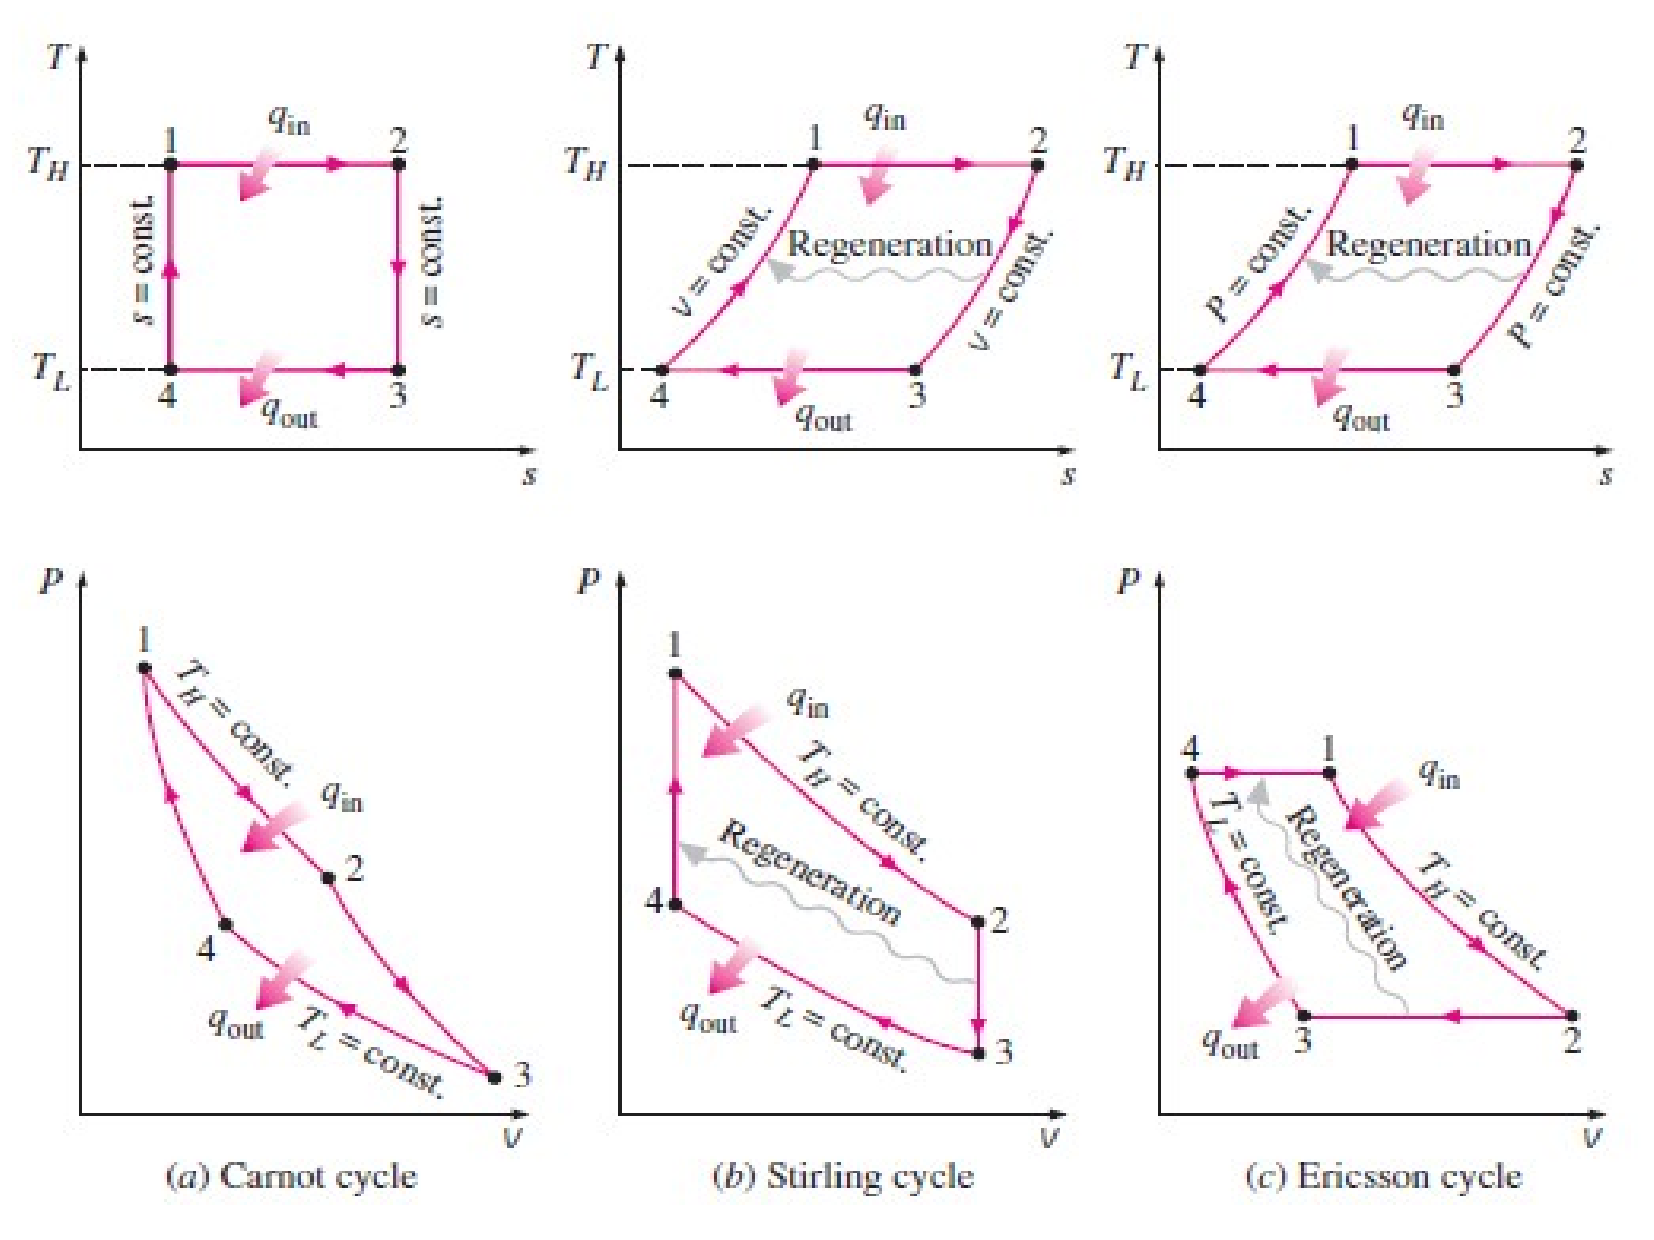
\includegraphics[width=6.cm,clip]{./Pics/InternalCombustion_StirlingEricssonCarnot}
     \end{center}
    \end{figure}   
   \end{column}  
  \end{columns}
\end{frame}



%%%
%%% Slide
%%%
\begin{frame}
 \frametitle{Stirling and Ericsson Cycles}
    \begin{itemize}
     \item <1-> Stirling and Ericsson cycles are totally reversible and, if operated between the same temperature limits, have the same efficiency as the Carnot cycle:
      \begin{displaymath}
       \eta_{\text{Stirling}}=\eta_{\text{Ericsson}}=\eta_{\text{Carnot}}=1-\frc{T_{L}}{T_{H}}
      \end{displaymath}
     \item <2-> Stirling and Ericsson cycles are difficult to achieve in practice because they involve heat transfer through a differential temperature difference in all components including the regenerator;
     %\item <3-> This would require providing infinitely large surface areas for heat transfer or allowing an infinitely long time for the process. Neither is practical. In reality, all heat transfer processes occur through a finite temperature difference, the regenerator does not have an efficiency of 100 percent, and the pressure losses in the regenerator are considerable.
     \item <3-> They are \textcolor{blue}{external combustion engines}, i.e., the fuel is burned outside the cylinder -- different from gasoline of diesel engines in which fuel is burned inside the cylinder;
     \item <4-> In external combustion, a variety of fuels can be used as a source of thermal energy;
     \item <5-> Also, there is more time for combustion and therefore the combustion process is more complete leading to less pollution and more energy extraction from the fuel.
     %\item <6-> Finally,  these engines operate on closed cycles, and thus a working fluid that has the most desirable characteristics (stable, chemically inert, high thermal conductivity) can be utilised as the working fluid. Hydrogen and helium are two gases commonly employed in these engines. Despite the physical limitations and impracticalities associated with them, both the Stirling and Ericsson cycles give a strong message to design engineers: Regeneration can increase efficiency. It is no coincidence that modern gas-turbine and steam power plants make extensive use of regeneration.
  \end{itemize}
\end{frame}

\subsection{Summary}
%%%
%%% Slide
%%%
\begin{frame}
 \frametitle{Summary}
 \begin{enumerate}
  \item <1-> Combustion engines:
  \begin{enumerate}
    \item <2-> Internal: Otto, Diesel, Dual Combustion and Atkinson cycles;
    \item <3-> External: Stirling and Ericsson;
  \end{enumerate}
  \item <4-> Stages on 2- and 4-strokes internal combustion engines;
  \item <5-> Thermal analysis of the cycles -- comparison {\it via} air-standard efficiency;
  \item <6-> Sensitivity analysis of internal combustion cycles;
  \item <7-> Brief summary of external combustion cycles.
 \end{enumerate}
\end{frame}


\end{document}
